\documentclass[final,12pt,twoside]{book}
\usepackage[]{manuscriptThese}

\graphicspath{{eps/}}

\usepackage{tikz}


\usetikzlibrary{trees,patterns,matrix,arrows,backgrounds}
%\tikzstyle{every node}=[draw=black,thick,anchor=west]
\tikzstyle{everynode}=[draw=black,thick,anchor=west]
\tikzstyle{selected}=[draw=red,fill=red!30]
\tikzstyle{optional}=[dashed,fill=gray!50]





\usepackage{pgfplots}
   \usepgfplotslibrary{dateplot}
 \pgfplotsset{width=7cm,compat=1.3}
 \usepackage{pgfplotstable}
   \pgfplotstableset{col sep=comma}

\usetikzlibrary{arrows,arrows.meta,chains,calc,trees,positioning}
\definecolor{lavander}{cmyk}{0,0.48,0,0}
\definecolor{violet}{cmyk}{0.79,0.88,0,0}
\definecolor{burntorange}{cmyk}{0,0.52,1,0}
\definecolor{lightblue}{cmyk}{0.85,0.5,0,0}

\def\lav{red!80}
\def\oran{gray!30}

\tikzstyle{peers}=[draw,circle,violet,bottom color=\lav,
top color= white, text=violet,minimum width=7pt]

\tikzstyle{superpeers}=[draw,circle,burntorange, left color=\oran,
text=violet,minimum width=17pt]

\tikzstyle{servers}=[draw,circle,blue, left color=lightblue,
text=black,minimum width=25pt]

\tikzstyle{legendsp}=[rectangle, draw, burntorange,
thin,bottom color=\oran, top color=white,
text=black, minimum width=2.5cm]

\tikzstyle{legendp}=[rectangle, draw, violet,  thin,
bottom color=\lav, top color= white,
text= black, minimum width= 2.5cm]

\tikzstyle{legends}=[rectangle, draw, violet,  thin,
bottom color=lightblue, top color= white,
text= black, minimum width= 2.5cm]

\tikzstyle{legend_general}=[rectangle, 
minimum width=2.5cm, minimum height=0.8cm]



\definecolor{bleue}{RGB}{66,200,244}
\definecolor{rouge}{rgb}{0.96,0.23,0.37}
\definecolor{vert}{RGB}{78,244,66}
\tikzset{%
	>={Latex[width=2mm,length=2mm]},
	% Specifications for style of nodes:
	base/.style = {rectangle, rounded corners, draw=black,  text centered,text 
	opacity=1},
	rejected/.style = { text=rouge},
	end/.style = {base, fill=vert!20},
	process/.style = {base, minimum width=5.5cm},
	event/.style = {base,minimum height=1.7cm},
	eventn/.style = {base,minimum height=1.7cm,fill=vert!20},
	eventc/.style = {base,minimum height=1.7cm, fill=rouge!20}
}


\usepackage{xcolor}
\colorlet{punct}{red!60!black}
\definecolor{background}{HTML}{EEEEEE}
\definecolor{delim}{RGB}{20,105,176}
\colorlet{numb}{magenta!60!black}

\lstdefinelanguage{json}{
	basicstyle=\small\normalfont\ttfamily,
	numbers=left,
	numberstyle=\scriptsize,
	stepnumber=1,
	numbersep=8pt,
	xleftmargin=4ex,
	showstringspaces=false,
	breaklines=true,
	tabsize=1,
	frame=lines,
	%backgroundcolor=\color{background},
	string=[s]{"}{"},
	stringstyle=\color{blue},
	comment=[l]{:},
	commentstyle=\color{black},
	literate= 
	{\{}{{{\color{delim}{\{}}}}{1}
	{\}}{{{\color{delim}{\}}}}}{1}
	{[}{{{\color{delim}{[}}}}{1}
	{]}{{{\color{delim}{]}}}}{1}
	{,}{{{\color{punct}{,}}}}{1}
}
\makeglossaries

\title{Architecture évènementielle pour les Environnements Virtuels 
	Collaboratifs 
	sur le web : Application à la manipulation et à la 
	visualisation d'objets 3D}
\author{Caroline Desprat}	

%\usepackage[hide=true]{nobibprint}
\begin{document}
	\frontmatter
	%!TEX root = _main.tex
%definition glossaire

\newacronym[longplural={Application Programming 
Interfaces},plural=APIs]{API}{API}{Application Programming Interface}
\newacronym{SVG}{SVG}{Scalable Vector Graphics}
\newacronym{SIG}{SIG}{Système d'Information Géographique}
\newacronym{CSS}{CSS}{Cascading Style Sheet}

\newacronym{RRTCC}{RRTCC}{Receiver-side Real-Time Congestion 
Control}


\newacronym{DTLS}{DTLS}{Datagram Transport Layer Security}
\newacronym{WebRTC}{WebRTC}{Web Real-Time Communication}
\newacronym{NAT}{NAT}{Network Address Translator}
\newacronym{STUN}{STUN}{Simple Traversal of UDP through NATs}
\newacronym{TURN}{TURN}{Traversal Using Relays around NAT}
\newacronym{CSCW}{CSCW}{Computer-Supported 
	Cooperative Work}

\newacronym[longplural={Environnements Virtuels Collaboratifs},plural=EVCs]{EVC}{EVC}{Environnement Virtuel Collaboratif}

\newacronym[longplural={Environnements Virtuels},plural=EVs]{EV}{EV}{Environnement Virtuel}

\newacronym[longplural={Environnements Virtuels Collaboratifs 3D},plural=EVCs 3D]{EVC3D}{EVC 3D}{Environnement Virtuel Collaboratif 3D}
\newacronym[firstplural=Environnements Virtuels 3D (EV 3D),plural=EV 3D]{EV3D}{EV 3D}{Environnement Virtuel 3D}
\newacronym[longplural={Collaborative Virtual Environments},plural=CVEs]{CVE}{CVE}{Collaborative Virtual 
Environment}
\newacronym{RV}{RV}{Réalité Virtuelle}
\newacronym{ICE}{ICE}{Interactive Connectivity Establishment}
\newacronym[longplural={Systèmes d'Edition Collaborative en 
P2P},plural={SEC P2P}]{SECP2P}{SEC P2P}{Système d'Edition 
Collaborative en P2P}
\newacronym[longplural={Systèmes d'Edition Collaborative},plural=SEC]{SEC}{SEC}{Système d'Edition Collaborative}

\newacronym{CE}{CE}{cohérence éventuelle}
\newacronym{LAN}{LAN}{Local Area Network}
\newacronym{WAN}{WAN}{Wide Area Network}

\newacronym{PLM}{PLM}{Product Lifecycle Management}
\newacronym{PDM}{PDM}{Product Data Management}

\newacronym{DDS}{DDS}{Data Distribution Service}

\newacronym{UDP}{UDP}{User Datagram Protocol}
\newacronym{CAO}{CAO}{Conception Assistée par Ordinateur}
\newacronym{BIM}{BIM}{Business Information Modeling}

\newacronym{BSP}{BSP}{Binary Space Partitioning}
\newacronym{CSG}{CSG}{Constructive Geometry Solid}

\newacronym{3D}{3D}{tridimension}
\newacronym{CAP}{CAP}{Consistency, Availability, and Partition Tolerance}
\newacronym{CDP}{CDP}{Cohérence, Disponibilité, et Tolérance au partitionnement}

\newacronym{TLS}{TLS}{Transport Layer Security}
\newacronym{TCP}{TCP}{Transmission Control Protocol}
\newacronym{STCP}{STCP}{Stream Control Transmission Protocol}
\newacronym{SCTP}{SCTP}{Stream Control Transmission Protocol}
\newacronym{W3C}{W3C}{World Wide Web Consortium}
\newacronym{IETF}{IETF}{Internet Engineering Task Force}
\newacronym{P2P}{P2P}{pair à pair}
\newacronym{GPU}{GPU}{Graphic Processing Unit}
\newacronym{CPU}{CPU}{Central Processing Unit}
\newacronym{JSON}{JSON}{JavaScript Object Notation}
\newacronym{DOM}{DOM}{Document Object Model}
\newacronym{BSON}{BSON}{Binary JSON}
\newacronym{glTF}{glTF}{GL Transmission Format}
\newacronym{OWL}{OWL}{Web Ontology Language}
\newacronym{BI}{BI}{Business Intelligence}
\newacronym[longplural={Operational Transformations }, 
plural=OTs]{OT}{OT}{Operational Transformation}
\newacronym[longplural={Commutative Replicated Data 
Types },plural=CRDTs]{CRDT}{CRDT}{Conflict-Free Replication Data 
Type}
\newacronym[longplural={Uniform Resource Identifiers},plural=URIs]{URI}{URI}{Uniform Resource Identifier}


 \newglossaryentry{XHR}{
	name=XHR,
	description={(abbréviation pour XMLHttpRequest) est un objet du navigateur accessible en JavaScript qui permet d'obtenir des données à l'aide de requêtes HTTP}
}
 \newglossaryentry{SIP}{
	name=SIP,
	description={(abbréviation pour Session Initiation Protocol) est est un protocole standard ouvert de gestion de sessions.}
}


\newacronym{HTML}{HTML}{HyperText Markup Langage}
\newacronym{JS}{JS}{JavaScript}
\newacronym{PubSub}{PubSub}{Publish-Subscribe}
\newacronym{ES}{ES}{Event Sourcing}
\newacronym{CS}{CS}{Command Sourcing}
\newacronym{CQRS}{CQRS}{Command Query Responsability Segregation}
\newacronym{EP}{EP}{event processing}
\newacronym{CCI}{CCI}{Causality, Convergence, Intention}

\newacronym{CDN}{CDN}{Content Delivery Network}
\newacronym{EDA}{EDA}{Event-Driven Architecture}

\newacronym{DDD}{DDD}{Domain Driven Design}
\newacronym{UI}{UI}{User Interface}
\newacronym{IU}{IU}{Interface Utilisateur}
\newacronym{IHM}{IHM}{Interface Homme Machine}
\newacronym{AIC}{AIC}{Architecture, Ingénierie et Construction}
\newacronym{ORM}{ORM}{Object-Relational Mapping}

\newacronym{NoSQL}{NoSQL}{Not Only SQL}
\newacronym{RTP}{RTP}{Real-Time Transport Protocol}
\newacronym{RTCP}{RTCP}{Real-time Transfert Control Protocol}
\newacronym{CEP}{CEP}{Complex Event Processing}
\newglossaryentry{WebSocket}{
	name=WebSocket,
	description={Protocole réseau standard du Web visant à créer des canaux de communication full-duplex par dessus une connexion TCP}
}

\newglossaryentry{cloud}{
	name=cloud,
	description={Définir le cloud}
}
\newglossaryentry{EventStore}{
	name=event store,
	description={Mémoire permettant le stockage des évènements en mode 
	"\textit{append-only}"}
}

\newglossaryentry{snapshot}{
	name=Snapshot,
	description={(contexte : CQRS) Instantané de l'état d'un agrégat convertissant 
	l'objet du domaine en un objet de transferts de données (DTO)}
}
\newglossaryentry{RTPdef}
{
	name=Real-Time Transport Protocol,
	description={est un protocole de 
		communication permettant le transport de données soumises à des 
		contraintes de temps réel (flux média audio ou vidéo). Le protocole 
		ajoute un en-tête spécifique aux paquets UDP pour spécifier le type et 
		le format (codec) du média transporté, numéroter les paquets, et fournir 
		une indication d'horloge.}
}

\newglossaryentry{RTCPdef}
{
	name=Real-time Transfert Control Protocol,
	description={est un protocole de contrôle des flux \gls{RTP} qui transmet de 
		manière périodique par tous les participants des paquets de contrôle sur 
		une session (informations basiques sur les participants d'une session, sur 
		la qualité de service)}
}


\newglossaryentry{streaming3D}{
	name=Streaming 3D,
	text={streaming 3D},
	description={est une technique permettant d'envoyer un contenu 3D sous la forme d'un flux continu par le biais d'internet, qui peut être utilisé/lu au fur et à mesure qu'il est reçu}
               }

               \newglossaryentry{framework}{
	name=Framework,
	text={framework},
	plural={frameworks},
	description={(ou structure logicielle en français) est un ensemble de composants génériques proposant un cadre de travail guidant l'architecture logicielle}
               }
               
               
               \newglossaryentry{workflow}{
               	name=Workflow,
               	text={workflow},
               	plural={workflow},
               	description={(ou flux de travaux en français) est la représentation d'une suite d'opérations effectuées par une entité (personne, groupe\ldots). L'expression renvoie au passage d'une ressource d'une étape à l'autre}
               }
               
              \newglossaryentry{computer}{
	name=computer,
	description={is a programmable machine that receives input,
               stores and manipulates data, and provides
               output in a useful format}
               }

   
              \newglossaryentry{NATT}{
              	name=NAT Traversal,
              	description={est une technique pour établir et maintenir les connexions internet à travers les passerelles qui implémentent \gls{NAT}. \gls{NAT} casse le principe de connectivité de bout en bout originalement envisagée lors de la conception d'internet.}
              }
          
                        \newglossaryentry{ICEF}{
          	name=ICE Framework,
          	description={est une technique dans le domaine du réseau pour trouver le chemin entre deux machine pour communiquer l'une avec l'autre, le plus directement possible en P2P. Le framework permet aux pairs en cours d'établissement de connexion de découvrir et communiquer leur adresse IP publique dans le but de pouvoir être atteint par d'autres pairs.}
          }

          
              
             
	\maketitle
	\dominitoc
	%!TEX root = _main.tex
\clearpage
%\addcontentsline{toc}{chapter}{Résumé}
%\adjustmtc
\section*{Résumé}

L’évolution technologique du web durant ces dernières années a favorisé l’arrivée d’environnements virtuels collaboratifs pour la modélisation 3D à grande échelle. Alors que la collaboration réuni dans un même espace partagé des utilisateurs distants géographiquement pour un objectif de collaboration commun, les ressources matérielles qu'ils apportent (calcul, stockage, 3D ...) avec leurs connaissances sont encore trop rarement utilisées et cela constitue un défi. Il s'agit en effet de proposer un système simple, performant et transparent pour les utilisateurs afin de permettre une collaboration efficace à la fois sur le volet computationnel mais aussi, bien entendu, sur l'aspect métier lié à la modélisation et la visualisation 3D dans un environnement hétérogènes en termes de performances de calcul, de rendu et de connexion.
Pour rendre efficace le passage à l’échelle, en conservant une source de vérité centralisée, de nombreux systèmes utilisent une architecture réseau dite "hybride", combinant client serveur et pair-à-pair. Cependant, la synchronicité élevée et la réplication des données sur tous les sites peut mener à une divergence des copies dans un environnement réparti. C’est pourquoi il est nécessaire de s’intéresser à la réplication optimiste adaptée aux propriétés ces environnements collaboratifs 3D : la dynamicité des utilisateurs et leur nombre, le type de donnée traitées (3D) et leur masse. Le cadre d’un système collaboratif impose également la conservation des propriétés de Causalité, Convergence et préservation de l’Intention (CCI).

Cette thèse présente un modèle pour les systèmes d’édition collaborative en 3D dans un environnement web. Dans ce modèle est intégrée une architecture cliente (3DEvent) qui permet de déporter les aspects métiers de la 3D au plus près de l’utilisateur sous la forme d’évènements. La mise en place de cette architecture basée-évènements repose sur le constat d’un fort besoin de traçabilité et d’historique sur les données 3D lors de l’assemblage d’un modèle. Cet aspect est porté intrinsèquement par le patron de conception event-sourcing. Ce modèle est complété par la définition d’un intergiciel en pair-à-pair. Sur ce dernier point, nous proposons d'utiliser une technologie récente comme WebRTC qui présente une API familière aux développeurs de services en infonuagique. Une évaluation portant sur deux études utilisateur concernant l’acceptance du modèle proposé a été menée dans le cadre de tâches d’assemblage de modèles 3D sur plusieurs groupes d’utilisateurs.

\paragraph{Mot clés : }environnement virtuel collaboratif, réseau pair-à-pair, WebRTC, web 3D, conception 3D, traitement réparti évènementiel, architecture hybride, event-sourcing.
\pagebreak
\section*{Abstract}

Web technologies evolutions during last decades fostered the development of 
collaborative virtual environments for 3D design at large scale. Despite the fact 
that collaborative environments gather in a same shared space geographically 
distant users in a common objective, the hardware ressources of their clients (calcul, 
storage, graphics ...) are often underused because of the challenge it represents. It is indeed 
a matter of offering an easy-to-use, efficient and transparent collaborative system 
to the user supporting both computationnal and 3D design visualisation and 
business logic needs in heterogeneous environments in terms of computing, 
rendering and connexion performances. To scale well while conserving a 
centralised authoritative source of data, numerous systems use a network 
architecture called "hybrid", combining both client-server and peer-to-peer. 
However, real-time updates and data replication on different sites lead to 
divergence of copy in such a distributed environment. That is why optimistic 
replication is well adapted to 3D collaborative envionments by taking into account 
different parameters: the dynamicity of users and their numbers, the 3D data type 
used and the large amount and size of it. It is also imperative to respect 
collaborative system properties of Causality, Convergence and Intention 
preservation (CCI).

This document presents a model for 3D web-based collaborative editing systems. This model integrates 3DEvent, an client-based architecture allowing us to bring 3D business logic closer to the user using events. Indeed, the need of traçability and history awareness is required during 3D design especially when several experts are involved during the process. This aspect is intrinsec to event sourcing design pattern. This architecture is completed by a peer-to-peer middleware responsible for the synchronisation and the consistency of the system. To implement it, we propose to use the recent web standard API called WebRTC, close to cloud development services know by developers. To evaluate the model, two user studies were conducted on several group of users concerning its responsiveness and the acceptance by users in the frame of cooperative assembly tasks of 3D models.




\paragraph{Keywords: }collaborative virtual environment, peer-to-peer network, WebRTC, web 3D, 3D design, distributed event-based system, hybrid architecture, event-sourcing.

\pagebreak
	%%!TEX root = main.tex

\thispagestyle{empty}
\section*{Remerciements}
\addcontentsline{toc}{chapter}{Remerciements}
\adjustmtc

Je tiens tout d'abord à remercier les membres du jury pour avoir accepter de 
participer à ce comité, en particulier, les rapporteurs pour leurs commentaires 
pertinents et constructifs lors des pré-rapports.
\\

Ensuite, je tiens à remercier Hervé Luga, mon directeur de thèse, et Jean-Pierre 
Jessel, mon co-encadrant de thèse, pour l'encadrement qu'ils ont exercé durant 
ces trois ans (et onze mois), en m'accordant une grande confiance dans le choix 
et la réalisation du sujet de cette thèse. 
Hervé, qui depuis le stage de Master m'a suivie et donner la possibilité d'ouvrir 
ma recherche à d'autre champs disciplinaires. Jean-Pierre, qui a su distiller 
opportunités et ressources au cours de ma thèse pour voir au delà de la vie de 
laboratoire.
\\

Je crois avoir été un objet test de l'université fédérale de Toulouse entre mon 
université d'inscription et d'enseignement (UT2J), celle où se situait mon bureau 
(UT1-C) et celle des projets et des séminaires (UPS). Cela m'a permis de 
rencontrer de nombreuses personnes, collègues et amis formidables que je tiens 
également à remercier pour leur patience ainsi que pour les longs et passionnés 
échanges que nous avons eu. Je pense en particulier à la ME310, où l'ambiance 
chaleureuse 
(surtout l'été), a été le berceau de belles amitiés. {\color{white} Jean, Jiefu, 
Dennis, Audren, Arianna, David, Valentin, Fabien, Nicolas, Elodie, Nathalie.}

Les ami·e·s. Toi qui a relu un papier la veille pour le lendemain ou cette 
thèse sans n'y rien connaître, ou encore toi qui ne m'a pas posé la question \og 
alors c'est 
prévu pour quand la soutenance ?\fg{}, merci. {\color{white} Ada, Sof, Anabelle, 
Thomas, 
Laurent, Cev, Katia, Catherine et (Christian).}

Papounet, toujours présent même à distance. Les bons petits plats, les 
petits sms, les voyages\dots~Toujours sensibles, parfois 
silencieux, parfois musicaux, ces encouragements m'ont toujours donné des 
appuis sur lesquels me reposer. Merci.\\

Julia, sista 
d'amour, la motivation derrière cette thèse te doit beaucoup et moi aussi. En 
partageant l'expérience de thèse de l'une et l'autre nous avons appris beaucoup 
sur chacune. J'ai trouvé dans ma sœur chérie et adorée une femme brillante, 
disponible et spontanée. Merci.
\\

Benoît, je pense que tu n'envisageais pas cette aventure de cette manière. Moi 
non plus. Toujours là, 
patient, à m'écouter, me proposer des idées et à me soutenir. Ces 
moments de thèses partagés ensemble sont des morceaux de vie uniques que je 
suis heureuse d'avoir partagés avec toi. Merci.

\clearpage
\pagebreak

\thispagestyle{empty}
\vspace*{\stretch{1}}
\begin{flushright}
\textit{À maman,}
\end{flushright}
\vspace*{\stretch{2}}

\pagebreak

	\completetable
	\completelist
	
	\mainmatter

%\chapter{Introduction}
%%!TEX root = main.tex
\chapter{Introduction}
\chaptertable
\section{Contexte}
Le besoin de collaboration et de manipulation en temps-réel d'objets en \gls{3D} 
ainsi que leur contrôle de version a été très tôt une raison de la dissémination des 
outils pour la \gls{CAO}. Tandis que l'ingénierie et la visualisation scientifique ont 
produit des quantités de données massives dans des domaines tels que la 
conception architecturale, l'industrie des jeux ou encore l'impression \gls{3D}, un 
besoin croissant de maintenir, visualiser et manipuler de larges scènes \gls{3D} 
polygonales pouvant être éditées par de multiples utilisateurs de manière 
concurrente se fait sentir \info{better read the first 
	one!}\cite{Chandrasegaran2013,Wu2014}. Or, la quantité et la taille des données 
étant toujours croissante, il devient de plus en plus difficile de partager les 
modèles, particulièrement avec les utilisateurs n'ayant pas accès aux derniers 
logiciels et matériels graphiques. C'est pourquoi nous observons un 
développement en forte progression de plateformes légères déployées sur le web 
permettant de répondre à ces besoins. 
Dans un \gls{EVC3D}, la simulation distribuée d'un environnement virtuel 3D, un 
grand nombre d'utilisateurs situés à différents endroits géographiques peuvent 
interagir les uns avec les autres en temps-réel. 
Cette distorsion de l'espace physique et temporel impose aux \gls{EVC3D} des 
mécanismes de communication rapide, conservant un environnement cohérent
des données partagées durant la collaboration. 
L'utilisation d'un client comme medium pour 
accéder à l'\gls{EVC3D} est requise pour envoyer des demandes au serveur. Le 
client peut être manipulé par un utilisateur ou un agent logiciel (bot).
Un \gls{EVC3D} se compose également un protocole de communication qui 
permet aux différents clients d'échanger les mises à jours correspondants aux 
modifications effectuées dans l'espace 3D virtuel partagé. La distribution des 
données devient alors un enjeu de taille dans ce type d'application en terme de 
temps, de sécurité et de fiabilité. 


%!TEX root = main.tex
%\chapter{Contexte}




\section{La collaboration}
La collaboration \info{https://wiki.p2pfoundation.net/Collaboration} est souvent 
définie \info{ref}comme un processus récursif
\footnote{Le « principe de boucle 
	récursive » se retrouve dans le concept de la pensée complexe. Edgar Morin  
	explique qu'« un processus récursif est un processus où les produits et les 
	effets 
	sont en même temps causes et producteurs de ce qui les produit » 
	\cite[p. 100]{Morin1990}.} où deux (ou plus) personnes (ou organisations) 
travaillent ensemble à la croisée de buts communs 
en partageant leurs connaissances pour apprendre et bâtir un consensus. 
La collaboration permet l'émergence de conceptions partagées dans la réalisation 
de visions partagées dans des environnements et des systèmes complexes. 
Les imbrications de chaque domaine et la transdiciplinarité sont acceptés comme 
dans le concept de pensée complexe. D'ailleurs, dans sa définition de la 
complexité, Edgar Morin fait référence au sens étymologique latin \og 
complexus\fg{} qui signifie \og ce qui est tissé ensemble\fg{} \cite{Morin1990a}.
La plupart des collaborations requièrent un élément dirigeant qui peut prendre une 
forme sociale (personne) au sein d'un groupe décentralisé et égalitaire (tout le 
monde au même niveau). L'élément dirigeant va souvent aider également trouver 
des consensus. 
La disponibilité des ressources peut également devenir un élément dirigeant dans 
la collaboration.
Une équipe travaillant de manière collaborative peut concentrer plus de 
ressources, de reconnaissances et de récompenses lors d'une 
compétition comportant des ressources finies. 
La collaboration est aussi présente dans la recherche de buts opposés mettant en 
avant la notion de collaboration contradictoire (en opposition avec la collaboration 
constructive) ; la négociation et la compétition peuvent également faire partie du 
terrain 
de la collaboration.

Une application collaborative peut aussi intégrer les notions de coordination et de 
coopération:
\begin{itemize}
	\item La \textbf{coordination} se base sur le principe d'harmonisation des 
	tâches, des rôles et du calendrier dans des systèmes et environnements 
	simples.
	\item La \textbf{coopération} permet de résoudre des problèmes dans des 
	systèmes et environnements complexes dans le les participants aurait été 
	incapables (temps, espace, connaissance, matériel) d'accomplir le travail seul.
\end{itemize}

Dans les années 2000, deux classifications ont été retenue concernant la 
collaboration.
La première classification, décrite en 2007 par Gotta \cite{Gotta2007}, propose 
un modèle segmentant la collaboration de manière structurée en quatre catégories 
: de la plus dirigée à la plus volontaire, en passant par l'hybride.
\begin{itemize}
	\item \textit{Collaboration centrée processus.} Les conditions requises du 
	processus 
	nécessitent l'engagement de l'utilisateur, qui doit, de part son rôle ou sa 
	responsabilité, diriger ses efforts dans la collaboration avec les autres. Cette 
	stratégie se concentre sur les activités de manipulation collaborative 3D plutôt 
	que sur leur contexte organisationnel afin de favoriser la synergie autour de la 
	réussite d'un processus. Par exemple, pour la création et l'utilisation d'un 
	modèle 	3D dans un \gls{BIM}, il s'agit de favoriser la prise de décision sur un 
	projet et 	communiquer à propos.
	
	\item \textit{Collaboration centrée activité}
	Les activités partagées créent un sentiment de co-dé\-pendance qui motive la 
	collaboration entre les membres. La co-dépendance prend l'avantage sur le 
	propre intérêt de chacun comme motivation pour collaborer. Le groupe a besoin 
	de chacun pour que l'objectif soit considéré comme réalisé. L'intérêt personnel 
	ou l'allégeance à l'esprit d'équipe peut aussi promouvoir la collaboration. Par 
	exemple, la visualisation collaborative des activités des différents contributeurs 
	dans l'\gls{EVC3D} permet à chacun de rendre compte de ses réalisations. Ce 
	type de collaboration doit beaucoup à l'ergonomie de l'activité qui insiste sur la 
	différence entre le travail prescrit et le travail réel : la tâche et l'activité.
	
	\item \textit{Collaboration centrée communauté.}
	La participation de la communauté à la collaboration induit la contribution. En 
	effet, les interactions professionnelles ou sociales peuvent encourager ou 
	persuader les utilisateurs de partager leurs informations ou connaissances 
	(exemple : les logiciels \textit{open-source})
	
	\item \textit{Collaboration centrée réseau.}
	Les connexions réseau favorisent la coopération réciproque. Dans le but de 
	récupérer des avis ou du savoir faire externe, un utilisateur peut faire appel à 
	son réseau social pour supplémenter une autre interaction collaborative. 
	Souvent utilisé dans le cadre d'urgences écologiques ou sanitaires (exemple: 
	contributions OpenStreetMap lors d'ouragan ou de tsunami), la collaboration 
	centrée réseau est très présente dans des situations l'expertise est fortement 
	valorisée comme dans les \gls{BIM} ou la visualisation scientifique, les 
	contributeurs peuvent être intégrés en fonction des besoins des utilisateurs déjà 
	présents sur le projet.
\end{itemize}
Dans le cadre de cette thèse, en se référant à cette première classification, les 
aspects centrés sur les activités sont mis en avant. En effet, la collaboration 
portant sur la modélisation 3D attend un résultat porté sur l'activité de conception. 
Celle-ci nécessite l'implication de personnes avec différentes compétences / 
connaissances qui doivent s'entraider pour parvenir à la mise en commun des 
objets 3D et réaliser leur objectif. \info{add figure}

Une seconde classification proposée par Callahan et al. 
\cite{Callahan2008} s'intéresse au triplé collaboration par équipe, collaboration 
communautaire, collaboration en réseau. En contraste avec la précédente 
classification qui se concentre sur les équipes et une collaboration formelle et 
structurée, celle-ci offre plus d'ouverture :
\begin{itemize}
	\item \textit{Collaboration par équipe.}
	Dans une équipe tous les membres se connaissent. Il y a une interdépendance 
	claire des tâches à effectuer où la réciprocité est attendue, avec un échéancier 
	et des objectifs explicites. Pour réaliser son but, l'équipe doit réaliser les tâches 
	dans un temps imparti. La collaboration par équipe suggère que les membres 
	coopèrent sur un pied d'égalité (bien qu'il y ait souvent un chef) recevant une 
	reconnaissance égale.
	
	\item \textit{Collaboration communautaire.}
	L'objectif de ce type de collaboration est plus orienté sur la possibilité 
	d'apprendre que sur la tâche elle-même, même si les centres d'intérêt sont 
	partagés par la communauté. Les utilisateurs sont là pour partager et construire 
	la connaissance plus que compléter un projet. Les membres vont aller voir leur 
	communauté pour demander de l'aide sur un problème ou un avis et ramener la 
	solution à implémenter dans leur équipe. L'adhésion peut être limitée et 
	explicite, mais les périodes de temps sont souvent ouvertes. Les membres 
	sont considérés comme égaux bien que les plus expérimentés peuvent avoir 
	des statuts privilégiés. La réciprocité est un facteur important dans la 
	communauté pour que cela fonctionne.
	
	\item \textit{Collaboration en réseau.}
	La collaboration en réseau est une sur-couche de la collaboration 
	traditionnellement centrée sur la relation d'une équipe ou d'une communauté. 
	Elle s'appuie sur une action individuelle et un intérêt personnel qui resurgissent 
	ensuite sur le réseau sous la forme de personnes qui contribuent ou cherchent 
	quelque chose à partir du réseau. L'adhésion et les périodes sont ouvertes et 
	non limitées. Il n'y a pas de rôle explicite. Les membres ne se connaissent pas 
	forcément. Le pouvoir est distribué. Cette forme de collaboration est dirigée par 
	l'avènement des réseaux sociaux, des accès à internet omniprésents et la 
	capacité de se connecter avec divers individus malgré la distance.
\end{itemize}
Cette thèse, en se référant à cette seconde classification, s'intéresse plutôt 
sur la collaboration par équipe. La conception d'un objet 3D et ses différentes 
phases de modélisation constitue une problématique nécessitant l'apport de 
plusieurs intervenants avec leurs capacités propres et travaillant de concert à la 
réalisation d'un objectif commun dans un temps imparti (exemple : revue de 
projet). Là où la coopération et l'effort conjoint pour réaliser un objectif sont 
nécessaires, le facteur temps reste un élément important à prendre en compte 
pour évaluer la productivité d'une session collaborative.

Le travail dans un \gls{EVC3D} facilite la compréhension 
de certaines problématiques liées à l'espace 3D ; c'est également un point de 
rencontre et d'échanges entre contributeurs sur le court terme et le long terme. 
Le croisement de ces deux dimensions, spatiale et temporelle, implique une 
multiplication des points de vue et donc des données à traiter sur le problème lors 
de la collaboration.

\subsection{Les systèmes collaboratifs}
\subsection{Les systèmes d'édition collaboratifs}
\subsubsection{Modèle d'édition collaborative}

\section{La collaboration 3D en accord avec l'évolution du web}

\subsection{Introduction}
\subsection{Le web et le P2P : WebRTC}
\subsection{Le web et la 3D :  WebGL}

\section{Les architectures évènementielles pour la collaboration}
\subsection{Sensibilisation lors de la collaboration}
\subsection{Intégration des contraintes métiers}


L'exigence vis-à-vis des temps de réponse est de plus en plus 
grande pour deux raisons principales : les limitations humaines (mémoire et 
attention limitées 
à court terme) et les aspirations de l'être humain (besoin d'être en contrôle sur les 
machines). S'accroissant au gré de la technologie et aux attentes 
utilisateurs (rétro-compatibilité, temps de 
chargement), elle varie selon le domaine mais reste très assez prégnante sur le 
web en général. 
Par exemple, dans un domaine annexe comme le e-commerce, une étude réalisée 
en 2006 explique qu’une grande partie des internautes abandonnaient leurs achats 
en ligne si les pages mettaient 4 secondes ou plus à charger. De nos jours, ce 
délai a été réduit au quart de seconde pour les grandes entreprises du web. Jakob 
Nielsen \cite{Nielsen1993a} indique trois temps de réponse limites concernant les 
temps de réponses :
\begin{itemize}
	\item \textit{0,1 seconde} donne une sensation de réponse instantanée, comme 
	si le 
	résultat avait été produit par l'utilisateur et non l'ordinateur. Ce niveau de temps 
	de réponse soutient la sensation de manipulation directe.\footnote{En IHM, la 
		manipulation directe correspond à un mode d'interaction au cours duquel les 
		utilisateurs font des actions sur les objets d'intérêt affichés dans l'interface 
		utilisateur en utilisant des actions physiques, incrémentales et réversibles 
		dont 
		les effets sont immédiatement visibles sur l'écran.} 
	\item \textit{1 seconde} garde le flux de pensées de l'utilisateur sans 
	interuption. 
	L'utilisateur peut ressentir un délai et par conséquent savoir que c'est la 
	machine qui génère le résultat ; l'utilisateur a quand même une impression de 
	contrôle sur l'expérience générale et peut de déplacer librement dans l'interface 
	sans attendre la machine. Ce degré de réactivité est impératif pour une bonne 
	navigation.
	\item \textit{10 secondes} conservent l'attention de l'utilisateur. Entre 1 et 10 
	secondes, l'utilisateur se sent dépendant de la machine, mais peut faire avec. 
	Au delà, l'utilisateur va commencer à penser à d'autres choses, rendant difficile 
	le retour à la tâche une fois que la machine répond.
\end{itemize} 
Dans le domaine de l'édition et la manipulation collaborative 
d'objets 3D, les contraintes abordées se situent à divers degrés : au chargement 
et lors des mises à jour. Le chargement concerne la phase de téléchargement de 
l'application web et des données relatives mais également d'affichage des 
modèles 3D sont spécifiques dans ce domaine car ils ont 
tendance à être lourds (structure de données 3D et métadonnées) à charger 
(contrairement au texte par exemple). Cette phase peut s'accorder des délais 
relativement long (1-10s) compte tenu du fait que l'utilisateur connaît en partie ces 
contraintes liées à la taille des objets 3D. Concernant les mises à jour, l'édition 
collaborative requiert un temps de réponse raisonnablement court est contraint par 
l'exactitude des calculs et le temps dans lequel le résultat est produit. Pour les 
mises à jour internes -- produites par l'utilisateur, actions sur l'interface -- on 
s'accordera sur un délai inférieur à 0,1 seconde dans cette thèse. 
Pour les mises à jour externes -- produites par les collaborateurs -- les latences 
réseaux rentrent en comptes (serveur, pairs\ldots) on s'accordera sur un délai 
entre 1 et 10 secondes dans cette thèse selon les degrés d'asynchronicité 
possibles. 



Les bureaux d'études en ingénierie et en architecture travaillent sur des projets 
(visualisation \gls{CAO}, \gls{BIM}, gestion et arrangement d'espaces 
architecturaux) qui 
nécessitent la collaboration de professionnels venant de milieux différents avec 
des compétences et connaissances variées. Les modifications dans leurs 
modèles en \gls{3D} doivent être revues par des gestionnaires de projet, des 
clients et les intervenants impliqués qui peuvent à leur tour suggérer des 
modifications sur la conception. Toutes ces entités ont besoin d'être capables de 
charger les ressources pour pouvoir les inspecter et les analyser. Ces contraintes 
se retrouvent dans le domaine du \gls{BIM}, l'architecture, l'héritage culturel, ou 
plus généralement dans des milieux transdisciplinaires concentrés sur la \gls{3D}. 
L'évolution de ces ressources passent par une visualisation et une manipulation 
collaborative efficace en terme de chargement de ressources et de transmission 
des mises à jour.




\section{Problématique}




Cette thèse se situe à l'interface de trois champs de recherches (Figure 
\ref{fig:problematique}). Le premier concerne les environnements de modélisation 
3D. Souvent commerciaux (Clara.io, OnShape, Verold Studio), les modeleurs 
utilisent des technologies supportée par les navigateurs web qui leur permettent 
d'être disponibles sur la plupart des plateformes. 
Cependant ces derniers reposent sur une gestion centralisée des données qui rend 
les utilisateurs très dépendants de la disponibilité de ces plateformes et d'une 
connexion internet pour la distribution des informations. 
Mises à part quelques exceptions, les fonctionnalités collaboratives 
sont souvent présentées comme mineures. Même si le \og partage\fg{} de la 
visualisation à la manière des \og réseaux sociaux\fg{} est assez courant, l'édition 
collaborative est souvent complexe à implémenter car les besoins sont nombreux. 
Parmi eux, on trouve tout d'abord le besoin d'avoir un système distribué 
conservant la cohérence des modifications de chacun des utilisateurs. Or, 
le nombre d'utilisateurs ne doit pas affecter l'expérience utilisateur ; le système 
doit supporter le passage à l'échelle. 
Le nombre d'utilisateurs élevé implique la mise en place d'un système de 
distribution de données adapté. Ce système est en plus contraint par la dynamicité
des arrivées et départs des collaborateurs (\textit{churn}) au cours d'une session. 
La dynamicité, qui ne permet pas d'avoir de pouvoir compter sur un nombre fixe de 
ressources, doit s'accorder avec les besoins variables en termes de ressources. 
Chaque client est porteur de ressources rarement complètement exploitées lors 
d'épisodes collaboratifs.

La visualisation et la manipulation collaborative d'objets \gls{3D} sont sujettes à 
plusieurs problématiques telles que la cohérence des ressources manipulées au 
cours du temps. Dans ce contexte, il existe un fort besoin de gérer l'évolution des 
versions permettant la revue des modèles \gls{3D}. 
En s'appuyant sur les ressources à dispositions, tels que les clients (navigateurs 
web) sur lesquels les utilisateurs manipulent les modèles \gls{3D}, le passage à 
l'échelle est plus flexible car les ressources augmentent avec le nombre de client 
et procurant également plus d'autonomie aux utilisateurs utilisant leurs ressources 
propres.
L'architecture de communication et les contraintes liées aux architectures 
distribuées et décentralisée correspond au second axe de recherche. 
Enfin, le dernier champs 
s'adresse à la partie que nous appellerons \og métier\fg{} qui se rapporte au 
domaine de la manipulation d'objets 3D qui inclue la 
gestion du cycle de vie des données 3D de l'interaction utilisateur à son stockage 
en passant par sa distribution. Ces aspects se rapportent principalement à 
l'historique, la traçabilité de l'information et l'expertise embarquée dans le système 
dans le cadre de cette thèse.

\begin{figure}[hbt]
	\centering
	\includegraphics[width=\columnwidth]{problematique.eps}
	\caption{Place de la contributions dans les différents champs de recherche}
	\label{fig:problematique}
\end{figure}

L'objectif de cette thèse est triple : 
\begin{enumerate*}[label=(\roman*)]
	\item extraire les informations liées aux règles métier pour l'affichage et la 
	manipulation d'objets \gls{3D} en collaboration nécessaires à la traçabilité de 
	l'information,
	\item repérer les principales problématiques de gestion des données sur le 
	réseau pour avoir une transmission efficace et transparente pour l'utilisateur,
	\item proposer un \gls{framework} pour un \gls{EVC3D} web intégrant ces 
	contraintes réseau, métier, et \gls{3D} dans un navigateur.
\end{enumerate*}
Dans le but d'achever de tels objectifs, voici les cinq Questions de Recherche 
posées :
\begin{description}
	\item[QR 1] Quelle architecture réseau est la plus adaptée pour une gestion 
	efficace, robuste et temps-réel des données \gls{3D} dans un environnement 
	web ?
	
	\item[QR 2] Quelle architecture logicielle confère une traçabilité des données 
	conforme aux règles métier liées à la manipulation d'objet \gls{3D} ? 
	
	\item[QR 3] Quels sont les mécanismes assurant à l'utilisateur d'être à la fois 
	autonome tout en ayant la possibilité de collaborer ?
	
	
	\item[QR 4] Comment faciliter l'implémentation d'un tel système en garantissant 
	le respect des règles métier liés à la manipulation d'objet \gls{3D}?
	
	\item[QR 5] Quelles sont les métriques (réseau, collaboration) permettant 
	d'évaluer un tel système de manière quantitative? qualitative? %Comment les 
	%utilisateurs recoivent la chose....
	
\end{description}

\section{Contributions}

La principale contribution de cette thèse est la définition et l'implémentation d'un 
ensemble de pratiques dans la gestion des données pour la manipulation d'objets 
3D de manière collaborative sur web. Cela est très utile pour la gestion de 
l'historique d'une scène \gls{3D} en utilisant des contenus \gls{3D} de différentes 
natures. Pour ce faire, j'ai choisi le paradigme événementiel et je l'ai 
intégré à mon modèle de collaboration grâce à l'utilisation de solutions 
préexistantes pour le partage et la diffusion de contenus \gls{3D} dans le cadre 
d'applications collaboratives sur le web.

La force motrice derrière ce travail a été le manque de processus et d'outils qui 
pourraient réellement supporter la modélisation collaborative \gls{3D} et la 
visualisation à l'échelle exigée par l'industrie, l'identification de problèmes 
spécifiques et leur formulation a également été importante. La recherche, 
cependant, introduit de nouveaux concepts dans le domaine de la gestion de 
données \gls{3D}. Les contributions de cette thèse peuvent être résumées comme 
suit.


\subsection{Contributions théoriques}

\begin{itemize}
	\item \improve{réécrire + introduire ref chapitre}Proposition d'un système de 
	gestion et de visualisation de contenu \gls{3D} avec un historique non linéaire 
	orienté évènements
	\item Définition d'une architecture hybride (client serveur et \gls{P2P}) adapté à 
	la distribution de contenus \gls{3D} dans le cadre d'une collaboration sur web en 
	temps-réelle.
	\item Introduction des concepts d'évènements métiers liées à la \gls{3D} 
	comme moyen d'interagir dans une scène  \gls{3D} multi-échelle
\end{itemize}
\subsection{Contributions pratiques}
\begin{itemize}
	\item \improve{réécrire + introduire ref chapitre}Définition d'une API ouverte et 
	de l'application cliente utilisation les principes et les technologies du web.
	\item Implémentation d'un prototype 3DEvent Client et de son évaluation 
	utilisateur 
	\item Implémentation d'un prototype 3DEvent Architecture et de son évaluation
	
\end{itemize}

%\bibentry{Desprat2017}

\section{Organisation du manuscrit}

%\section*{Organisation du manuscrit}
La présence de la \gls{3D} et des environnements virtuels collaboratifs \gls{3D} est 
de plus en plus présents dans l'industrie de la \gls{CAO} nécessitant de nouveaux 
modèles, outils et méthodes facilitant la mobilité et l'autonomie des utilisateurs. Il 
est aussi important de noter que le contenu multimédia \gls{3D} est aussi de plus 
en plus présent dans notre quotidien. Pour tout cela il est important de développer 
de nouveaux outils pour créer manipuler et partager du contenu \gls{3D}.
Le chapitre \info{ref chapitre} présente une architecture de communication hybride 
permettant de faciliter la transmission des objets \gls{3D} en temps réel de 
manière transparente pour l'utilisateur. La création d'\gls{EVC3D} sur le web à 
besoin de nouvelles architectures tirant partie des nouveaux standards du 
\gls{W3C}. Puis, le chapitre \info{ref cqrs} présente deux \info{2 contrib cqrs à 
	identifier} contributions reposant sur l'architecture cliente de 3DEvent pour 
manipuler des objets \gls{3D} avec une grande traçabilité et de manière autonome. 
%La première contribution propose 
Finalement, le chapitre\info{ref chap final} adresse le problème et la spécificité de 
la transmission du contenu \gls{3D} lors de session collaborative en temps-réel. 
En considérant et développant un modèle orienté évènements, 3DEvent dérive 
des 
stratégies pour délivrer et obtenir une scène 3D en continu (\textit{streaming} en 
anglais) en s'appuyant sur les différentes configurations matérielles, utilisateurs, 
réseaux.

%\chapter{Contexte}
%%!TEX root = main.tex
%\chapter{Contexte}




\section{La collaboration}
La collaboration \info{https://wiki.p2pfoundation.net/Collaboration} est souvent 
définie \info{ref}comme un processus récursif
\footnote{Le « principe de boucle 
	récursive » se retrouve dans le concept de la pensée complexe. Edgar Morin  
	explique qu'« un processus récursif est un processus où les produits et les 
	effets 
	sont en même temps causes et producteurs de ce qui les produit » 
	\cite[p. 100]{Morin1990}.} où deux (ou plus) personnes (ou organisations) 
travaillent ensemble à la croisée de buts communs 
en partageant leurs connaissances pour apprendre et bâtir un consensus. 
La collaboration permet l'émergence de conceptions partagées dans la réalisation 
de visions partagées dans des environnements et des systèmes complexes. 
Les imbrications de chaque domaine et la transdiciplinarité sont acceptés comme 
dans le concept de pensée complexe. D'ailleurs, dans sa définition de la 
complexité, Edgar Morin fait référence au sens étymologique latin \og 
complexus\fg{} qui signifie \og ce qui est tissé ensemble\fg{} \cite{Morin1990a}.
La plupart des collaborations requièrent un élément dirigeant qui peut prendre une 
forme sociale (personne) au sein d'un groupe décentralisé et égalitaire (tout le 
monde au même niveau). L'élément dirigeant va souvent aider également trouver 
des consensus. 
La disponibilité des ressources peut également devenir un élément dirigeant dans 
la collaboration.
Une équipe travaillant de manière collaborative peut concentrer plus de 
ressources, de reconnaissances et de récompenses lors d'une 
compétition comportant des ressources finies. 
La collaboration est aussi présente dans la recherche de buts opposés mettant en 
avant la notion de collaboration contradictoire (en opposition avec la collaboration 
constructive) ; la négociation et la compétition peuvent également faire partie du 
terrain 
de la collaboration.

Une application collaborative peut aussi intégrer les notions de coordination et de 
coopération:
\begin{itemize}
	\item La \textbf{coordination} se base sur le principe d'harmonisation des 
	tâches, des rôles et du calendrier dans des systèmes et environnements 
	simples.
	\item La \textbf{coopération} permet de résoudre des problèmes dans des 
	systèmes et environnements complexes dans le les participants aurait été 
	incapables (temps, espace, connaissance, matériel) d'accomplir le travail seul.
\end{itemize}

Dans les années 2000, deux classifications ont été retenue concernant la 
collaboration.
La première classification, décrite en 2007 par Gotta \cite{Gotta2007}, propose 
un modèle segmentant la collaboration de manière structurée en quatre catégories 
: de la plus dirigée à la plus volontaire, en passant par l'hybride.
\begin{itemize}
	\item \textit{Collaboration centrée processus.} Les conditions requises du 
	processus 
	nécessitent l'engagement de l'utilisateur, qui doit, de part son rôle ou sa 
	responsabilité, diriger ses efforts dans la collaboration avec les autres. Cette 
	stratégie se concentre sur les activités de manipulation collaborative 3D plutôt 
	que sur leur contexte organisationnel afin de favoriser la synergie autour de la 
	réussite d'un processus. Par exemple, pour la création et l'utilisation d'un 
	modèle 	3D dans un \gls{BIM}, il s'agit de favoriser la prise de décision sur un 
	projet et 	communiquer à propos.
	
	\item \textit{Collaboration centrée activité}
	Les activités partagées créent un sentiment de co-dé\-pendance qui motive la 
	collaboration entre les membres. La co-dépendance prend l'avantage sur le 
	propre intérêt de chacun comme motivation pour collaborer. Le groupe a besoin 
	de chacun pour que l'objectif soit considéré comme réalisé. L'intérêt personnel 
	ou l'allégeance à l'esprit d'équipe peut aussi promouvoir la collaboration. Par 
	exemple, la visualisation collaborative des activités des différents contributeurs 
	dans l'\gls{EVC3D} permet à chacun de rendre compte de ses réalisations. Ce 
	type de collaboration doit beaucoup à l'ergonomie de l'activité qui insiste sur la 
	différence entre le travail prescrit et le travail réel : la tâche et l'activité.
	
	\item \textit{Collaboration centrée communauté.}
	La participation de la communauté à la collaboration induit la contribution. En 
	effet, les interactions professionnelles ou sociales peuvent encourager ou 
	persuader les utilisateurs de partager leurs informations ou connaissances 
	(exemple : les logiciels \textit{open-source})
	
	\item \textit{Collaboration centrée réseau.}
	Les connexions réseau favorisent la coopération réciproque. Dans le but de 
	récupérer des avis ou du savoir faire externe, un utilisateur peut faire appel à 
	son réseau social pour supplémenter une autre interaction collaborative. 
	Souvent utilisé dans le cadre d'urgences écologiques ou sanitaires (exemple: 
	contributions OpenStreetMap lors d'ouragan ou de tsunami), la collaboration 
	centrée réseau est très présente dans des situations l'expertise est fortement 
	valorisée comme dans les \gls{BIM} ou la visualisation scientifique, les 
	contributeurs peuvent être intégrés en fonction des besoins des utilisateurs déjà 
	présents sur le projet.
\end{itemize}
Dans le cadre de cette thèse, en se référant à cette première classification, les 
aspects centrés sur les activités sont mis en avant. En effet, la collaboration 
portant sur la modélisation 3D attend un résultat porté sur l'activité de conception. 
Celle-ci nécessite l'implication de personnes avec différentes compétences / 
connaissances qui doivent s'entraider pour parvenir à la mise en commun des 
objets 3D et réaliser leur objectif. \info{add figure}

Une seconde classification proposée par Callahan et al. 
\cite{Callahan2008} s'intéresse au triplé collaboration par équipe, collaboration 
communautaire, collaboration en réseau. En contraste avec la précédente 
classification qui se concentre sur les équipes et une collaboration formelle et 
structurée, celle-ci offre plus d'ouverture :
\begin{itemize}
	\item \textit{Collaboration par équipe.}
	Dans une équipe tous les membres se connaissent. Il y a une interdépendance 
	claire des tâches à effectuer où la réciprocité est attendue, avec un échéancier 
	et des objectifs explicites. Pour réaliser son but, l'équipe doit réaliser les tâches 
	dans un temps imparti. La collaboration par équipe suggère que les membres 
	coopèrent sur un pied d'égalité (bien qu'il y ait souvent un chef) recevant une 
	reconnaissance égale.
	
	\item \textit{Collaboration communautaire.}
	L'objectif de ce type de collaboration est plus orienté sur la possibilité 
	d'apprendre que sur la tâche elle-même, même si les centres d'intérêt sont 
	partagés par la communauté. Les utilisateurs sont là pour partager et construire 
	la connaissance plus que compléter un projet. Les membres vont aller voir leur 
	communauté pour demander de l'aide sur un problème ou un avis et ramener la 
	solution à implémenter dans leur équipe. L'adhésion peut être limitée et 
	explicite, mais les périodes de temps sont souvent ouvertes. Les membres 
	sont considérés comme égaux bien que les plus expérimentés peuvent avoir 
	des statuts privilégiés. La réciprocité est un facteur important dans la 
	communauté pour que cela fonctionne.
	
	\item \textit{Collaboration en réseau.}
	La collaboration en réseau est une sur-couche de la collaboration 
	traditionnellement centrée sur la relation d'une équipe ou d'une communauté. 
	Elle s'appuie sur une action individuelle et un intérêt personnel qui resurgissent 
	ensuite sur le réseau sous la forme de personnes qui contribuent ou cherchent 
	quelque chose à partir du réseau. L'adhésion et les périodes sont ouvertes et 
	non limitées. Il n'y a pas de rôle explicite. Les membres ne se connaissent pas 
	forcément. Le pouvoir est distribué. Cette forme de collaboration est dirigée par 
	l'avènement des réseaux sociaux, des accès à internet omniprésents et la 
	capacité de se connecter avec divers individus malgré la distance.
\end{itemize}
Cette thèse, en se référant à cette seconde classification, s'intéresse plutôt 
sur la collaboration par équipe. La conception d'un objet 3D et ses différentes 
phases de modélisation constitue une problématique nécessitant l'apport de 
plusieurs intervenants avec leurs capacités propres et travaillant de concert à la 
réalisation d'un objectif commun dans un temps imparti (exemple : revue de 
projet). Là où la coopération et l'effort conjoint pour réaliser un objectif sont 
nécessaires, le facteur temps reste un élément important à prendre en compte 
pour évaluer la productivité d'une session collaborative.

Le travail dans un \gls{EVC3D} facilite la compréhension 
de certaines problématiques liées à l'espace 3D ; c'est également un point de 
rencontre et d'échanges entre contributeurs sur le court terme et le long terme. 
Le croisement de ces deux dimensions, spatiale et temporelle, implique une 
multiplication des points de vue et donc des données à traiter sur le problème lors 
de la collaboration.

\subsection{Les systèmes collaboratifs}
\subsection{Les systèmes d'édition collaboratifs}
\subsubsection{Modèle d'édition collaborative}

\section{La collaboration 3D en accord avec l'évolution du web}

\subsection{Introduction}
\subsection{Le web et le P2P : WebRTC}
\subsection{Le web et la 3D :  WebGL}

\section{Les architectures évènementielles pour la collaboration}
\subsection{Sensibilisation lors de la collaboration}
\subsection{Intégration des contraintes métiers}


%\chapter{État de l'art}
%%!TEX root = main.tex
\chapter{État de l'art}
\chaptertable

%\section{La visualisation et manipulation 3D collaborative sur web}

\section{Modélisation 3D collaborative sur le Web}

L'arrivée du web a bouleversé les usages liés à la collaboration sur des objets 3D. 
Les principes, les technologies, l'omniprésence du web en ont fait une plateforme 
de prédilection pour la visualisation et la manipulation d'objet 3D de haut niveau.   
Pour les projets d'\gls{AIC} ou de \gls{BIM}, la demande de traitement et la fidélité 
ont tendance à être plus élevés, particulièrement pour la représentation de dessins 
d'ingénierie ou de modèles d'architecture 3D. 
Les objets simples (primitives) ou les maillages optimisés pour le rendu temps-réel 
ne sont ni suffisants ni assez génériques pour être supportés par tous les 
processus liés à l'élaboration d'un produit. 
Plus les projets sont gros, plus ils dépendent d'une multitude de logiciels 3D --  
dont l'interopérabilité n'est pas garantie -- s'adressant chacun aux besoins d'une 
tâche spécifique. 
Chaque tâche (ex: modélisation \gls{CAO}, \textit{stress testing}\ldots) possède sa 
propre représentation des données qui peut varier selon les niveaux de 
sémantique attachés à la géométrie. 
Pour garder une trace de ces données et mettre en commun les données 
générées autour d'un produit, l'utilisation d'un \gls{PDM}/\gls{PLM} est 
souvent requise. Bien que certains outils de création d'objets 3D (par exemple 
Autodesk Revit) autorisent la synchronisation de fichier via leur dépôt à distance, 
ce n'est généralement pas applicable aux générations suivantes. 
En cela, une plateforme web pour un \gls{PDM}/\gls{PLM} à 
l'avantage d'être distribuée pour être accessible depuis un navigateur web ; avec 
un système d'édition hors-ligne, le téléversement peut s'avérer long et fastidieux.
De plus, les logiciels spécialisés pour la modélisation 3D, contrairement aux jeux 
multijoueurs, sont traditionnellement dédiés à un utilisateur unique sans 
représentation visuelle des autres opérateurs dans le même espace 3D. 
Ici encore, les principes d'accessibilité du web facilitent la création d'un espace 
virtuel 3D collaboratif pour la visualisation, la manipulation et l'échange de
données partagées. 
\subsection{HTML5 et au delà}
%TODO designing in context
%\cite{Dobos2015}

La collaboration en temps-réel est de plus en plus présente sur le web pour 
différents types de documents notamment 3D.
La revue sur la visualisation distribuée, effectuée par Grimstead et al. en 2005 
\cite{Grimstead2005}, indique que la plupart des systèmes sont conçus pour 
moins de cent 
utilisateurs simultanés et reposent sur un ou plusieurs serveurs pour supporter ces 
utilisateurs. 
Ils expliquent ce schéma par la volonté du fournisseur de service d'assurer une 
qualité de service et la sécurité du système. 
Les systèmes de \gls{RV} collaboratifs font exception à ce schéma où l'utilisation 
des réseaux \gls{P2P} est plus répandue pour supporter parfois plus d'un millier 
d'utilisateurs simultanés. 
Dans chacun des cas, chaque système a besoin d'un client adapté pour opérer de 
manière isolée sans inter-opérer avec les autre systèmes. 
C'est dans ce contexte qu'en 2011, Mouton et al. \cite{Mouton2011} présentent 
une analyse approfondie de l'état des environnements collaboratifs 3D, ciblant 
principalement la visualisation collaborative. 
Ils montrent l'apparition de la tendance à déporter les environnements collaboratifs 
sur le web grâce à l'évolution d'XMLHttpRequest en client-serveur et l'apparition du 
standard HTML5 comprenant un support avancé de l'audio et de la vidéo ainsi que 
plusieurs \gls{API} de stockage côté client (LocalStorage, IndexedDB). 
Les applications web revêtent plusieurs avantages par rapport aux applications 
natives sur mobiles ou aux logiciels autonomes. 
Cela repose principalement sur le fait que les navigateurs sont présents partout 
dans nos vies aujourd'hui (2017), incluant les téléphones intelligents et les 
tablettes qui les rendent indépendants des plateformes utilisées. 
Le déploiement sur le web ne requiert pas d'installation ou de mises à jour autre 
que celle du navigateur (en ne considérant que les applications sans greffon). 
La modification de l'application est gérée de manière centralisée par les serveurs 
qui distribuent l'application. 
Les éditeurs peuvent diffuser leur application à l'échelle mondiale instantanément  
et la mettre à disposition des utilisateurs sans dépendre d'un réseau de distribution 
autre qu'internet.

%Computer-Aided Engineering (CAE) Collaborative /


Parmi les solutions sans greffon (\textit{plugin less}), beaucoup sont développées 
pour faire de la modélisation 3D  et utilisent l'architecture client-serveur et le 
protocole 
\gls{WebSocket} pour effectuer la synchronisation entre les différents les clients 
collaborateurs. Quelques raisons peuvent expliquer cette situation :
\begin{enumerate}
	\item développement : connaissance du standard \gls{WebSocket} par les 
	développeurs (historique)
	\item gestion des données : simplification de la synchronisation des données 
	(centralisé)
	\item suivi de l'utilisateur : dépendance de l'utilisateur vis à vis de la connexion 
	au serveur et donc du service (engagement) 
\end{enumerate}

Parmi les solutions commerciales comme OnShape, Clara.io et TinkerCAD le 
choix de plateformes web dans l'infonuagique pour la modélisation \gls{CAO} est 
prépondérant souvent assorti d'un gestionnaire de version et d'une plateforme de 
diffusion des création.
OnShape est un service de modélisation 3D très riche dont l'objectif est de 
proposer une qualité équivalente des fonctionnalités de modeleurs autonomes 
(\textit{standalone}) professionnels, le tout de manière collaborative. Leur approche 
de la gestion de version développe le concept de micro version \cite{Baran2015}. 
Cette approche se retrouve dans les travaux de Lu et al.  \cite{Lu2016} qui l'utilisent pour gérer 
l'évolution de productions participatives liées à des tâches de modélisation 
3D grâce à  la créativité, l'intelligence et le savoir-faire 
d'un grand nombre de personnes en sous-traitance (\textit{crowdsourcing}). Le 
modeleur 3D Clara.io \cite{Houston2013} est plus généraliste. Il s'oriente 
davantage vers des fonctionnalités avancées de rendu 3D sur le \textit{cloud} en 
utilisant du lancer de rayons. 
Les fonctionnalités d'historisation et de collaboration proposées 
dans Clara.io restent très basiques (seulement annuler~/~refaire). TinkerCAD 
est aussi une plateforme de publication d'objets 3D pour faciliter l'accès à la 
conception d'objets 3D. TinkerCAD est une application destinée au grand 
public pour la conception et l'impression 3D. De ce fait, les fonctionnalités sont 
limitée à cause du métier, l'impression 3D et de la cible, grand public. La gestion 
de version est donc plus légère, similaire à celle proposée par Clara.io. 
OpenJSCAD, Verold Studio, Vectary sont d'autres 
exemples de modeleurs 3D moins connus avec des fonctionnalités proches de 
TinkerCAD.
Un peu à part, GrabCAD est une plateforme web plus orientée sur la gestion de 
données 3D \gls{CAO} (\gls{PLM}) qui possède un système de gestion de version 
performant et une système d'annotation et de visualisation collaborative.
Pour réduire l'empreinte mémoire des messages transmis lors de la collaboration 
sur le web, certains systèmes d'édition collaborative de contenu 3D utilisent une 
modélisation par surface implicite (BlobTree) \cite{Grasberger2013}. 
Les objets sont alors manipulés comme des géométries de construction de 
solides avec les opérations booléennes associées. 
Le Tableau \ref{table:encoding} résume les différents types 
d'encodage associé au type de modélisation 3D. 
\improve{tableau comparatif gestion historique ou versionning}
\improve{tableau comparatif de GrabCAD, OnShape, clara.io}
%
%\begin{table}[]
%	\centering
%	\caption{Comparaison de fonctionnalités entres modeleurs 3D basés web}
%	\label{my-label}
%	\begin{tabular}{@{}cccc@{}}
%		&  Client serveur & P2P &  Collaboratif\\ \midrule
%		Claro.io        & c        & g       & o       \\
%		GrabCAD                  & c        & g       & o       \\
%		OnShape &          &         &         \\
%		&          &         &         \\ \bottomrule
%	\end{tabular}
%\end{table}
\begin{table}[h]
	\centering
	\caption{Encodage des données transmises}
	\label{table:encoding}
	\begin{tabular}{@{}lcc@{}}\hline
		\textbf{Référence}& \textbf{Modélisation 3D}   & 
		\begin{tabular}[c]{@{}l@{}}\textbf{Encodage des}\\ 
			\textbf{modifications}\end{tabular} \\ \midrule
		\cite{Grasberger2013}        &      Blob (CSG)    & Fonction implicite        \\
		Clara.io \cite{Houston2013}               & Polygonale       &  Commande 
		interface     \\
		\cite{Mouton2014}                  & Polygonale       & Fonction paramétrique     \\
		OnShape \cite{Baran2015} &    Paramétrique      &     Microversion    \\
		cSculpt \cite{Calabrese2016} &      Polygonale    &    Fréquence spatiale  \\ 
		\bottomrule
	\end{tabular}
\end{table}

\subsection{Web 3D : deux approches}
La plateforme web possède certains avantages par rapport à des clients lourds. 
En effet, le développement de l'infonuagique a permis le développement de 
meilleures infrastructures de services. Du fait de ce développement, la création de 
plateformes collaboratives sur le web pour faire de la conception 3D est devenue 
non seulement faisable en termes de ressources mais également en termes de 
technologie. Il existe deux types d'approches pour créer du contenu web 2D ou 
3D. L'approche déclarative et l'approche impérative. La Figure \ref{fig:impdec} 
montre le pendant 3D pour chaque approche 2D. En 2D, les spécifications 
déclaratives (\gls{SVG}) et impératives (canvas) sont issues du \gls{HTML}5 alors 
qu'en 3D, les spécifications sont encore en évolution. 

\begin{figure}[hbt]
	\centering
	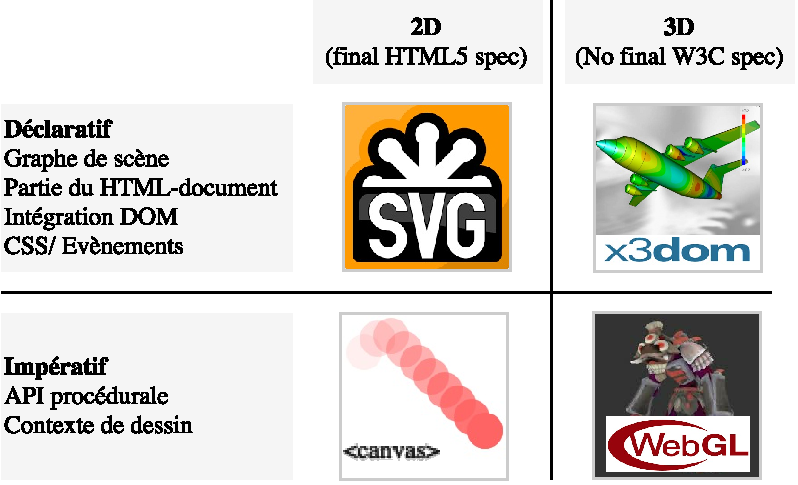
\includegraphics[width=0.7\columnwidth]{impdec}
	\caption{Déclaratif vs Impératif en 2D et en 3D sur le web}
	\label{fig:impdec}
\end{figure}

L'approche déclarative (Dec3D) s'intègre au \gls{DOM} et se 
focalise sur l'utilisation les technologies du web existantes comme CSS3, 
\gls{HTML}5 et l'Ajax. 
X3D est ainsi un format de fichier respectant le standard ISO \cite{X3D2011} pour 
représenter des scènes 3D interactives en XML, rétro-compatible avec VRML97. Il 
se différencie des formats de fichier type Collada en intégrant le comportement de 
la scène durant l'exécution en plus de la description du contenu 3D. Les deux 
bibliothèques les plus notables dérivées de ce standard sont X3DOM 
\cite{Behr2010} et XML3D \cite{Sons2010} : toutes les deux sont capables de 
supporter les récentes avancées de WebGL pour afficher une scène décrite dans 
le \gls{DOM} à l'intérieur d'un \textit{canvas} \gls{HTML}5. 
X3DOM essaye de respecter le standard X3D et ses concepts pour en permettre 
l'intégration du format dans le \gls{DOM}. De plus, X3DOM intègre le support 
d'élément \gls{HTML}, les évènements \gls{DOM} et de profils \acrshort{CSS} en 
supplément \cite{Sutter2015}. 
En comparaison avec X3DOM, XML3D a développé une extension à \gls{HTML}5 
pour décrire une scène 3D. 
L'utilisation d'un langage déclaratif basé sur XML comme X3D est bien 
adapté pour le contenu 3D utilise des données CAO/MAO ou WCS dans des 
applications \gls{SIG} car il peut être directement transformé (ex. XSLT) d'une 
représentation à une autre (tout comme le X3D peut être rendu dans un navigateur 
en utilisant X3DOM). 

L'approche déclarative est utilisée dans de nombreux travaux de visualisation 
scientifique 3D distribuée \cite{Jung2012} pour des données spatiales 
\cite{Stein2014} ou du rendu volumique \cite{Becher2012} par exemple. 
En manipulant directement les objets 3D à partir des éléments \gls{DOM}, grâce à 
sa structure bien connue, il est alors plus simple lors de la collaboration d'utiliser 
ces éléments \cite{Gadea2016} ou les évènements du \gls{DOM} \cite{Lowet2009} 
comme protocole de synchronisation de scènes. 
L'ajout de nombreux \textit{listeners} sur un document peut affecter les 
performances de parcours de l'arbre du \gls{DOM} notamment si une scène est
très peuplée.
%declarative XML- based languages such as X3D are suited well for SOAs in that 
%3D content, such as CAD/ CAM data or a given WCS response in a GIS 
%application, can be directly transformed, e.g. via an XSLT or similar transform, 
%from one representa- tion to another (such as an X3D world that can be rendered 
%in 
%real-time in the web browser using the X3DOM frame- work).

%TODO BIM CAD PLM 
%TODO Building Information Modeling: The Web3D Application for AEC 
%\cite{Campbell2007}
%TODO WEB3D, COLLABORATIVE DESIGN AND PLM Enrico Vezzetti (1), 
%Maria Grazia Violante (2)
%\info{webrtc collaborative visual analysis \cite{Li2015} }
%\info{webrtc medical \cite{Andrikos2015}}
%\info{webrtc x3dom \cite{Stein2014} \cite{Andrioti2015} }
%\info{webrtc webgl \cite{Desprat2015} \cite{Desprat2016} SAGE2 
%\cite{Marrinan2008} }

\begin{figure}[hbt]
	\centering
	\includegraphics[width=0.9\columnwidth]{webglstats.eps}
	\caption{Support de WebGL 1 (2014-2017) et WebGL 2 
		(2016-2017)}
	\label{fig:webglstats}
\end{figure}

Concernant l'approche impérative, la spécification WebGL 1.0 \cite{Khronos2011} 
proposée par le groupe Khronos permet aux navigateurs d'effectuer un rendu 3D 
grâce à une \gls{API} JavaScript adaptée de l'\gls{API} d'OpenGL~ES~2.0 
\cite{Khronos2007} en utilisant l'élément \textit{canvas} d'\gls{HTML}5. Cette 
spécification est supportée par la plupart des navigateurs traditionnels (Chrome 
depuis v49, Firefox depuis v52, Safari depuis v9.1, IE 11\footnote{Le contexte 
	WebGL est accessible depuis <<~\texttt{experimental-webgl}~>> au lieu de 
	<<~\texttt{webgl}~>>.\label{fn:webglcontext}}, Edge 14\textsuperscript{ 
	\ref{fn:webglcontext}} et Opera depuis v41) ainsi que les navigateurs mobiles 
	(iOS 
Safari depuis v9.3, Android Browser depuis v53 et Chrome for Android depuis v53) 
à l'exception d'Opera Mini\footnote{Données issues de 
	\url{http://caniuse.com/\#search=webgl}, consulté le 26/11/2016.}. La 
	spécification 
WebGL 2.0 \cite{Khronos2016} basée sur OpenGL~ES~3.0 \cite{Khronos2008}, 
déjà publiée en tant que brouillon, est en phase 
expérimentale\footnote{\url{http://caniuse.com/\#feat=webgl2} consulté le 
	26/11/2016}.\improve{add some example of coviz web} La Figure 
\ref{fig:webglstats} montre l'évolution du support de WebGL~1 et WebGL~2 durant 
ces dernières années sur les différentes plateformes possédant un navigateur 
web\footnote{Images capturées sur \url{https://webglstats.com/}. Les statistiques 
	sont collectées à partir de sites partenaires de \url{webglstats.com}. Ces sites 
	sont en 
	ciblent des néophytes de la WebGL possédant donc le matériel 
	dédié à la 3D en général. Consulté le 04/07/2017.}.

\section{Communication en temps-réel}
L'expression temps-réel est largement utilisé par des applications requérant une 
forme de temps de réponse rapide et réactif pour que l'utilisateur ait une bonne 
expérience. La communication dans un \gls{EVC} particulièrement pour permettre aux utilisateurs de s'immerger dans la collaboration et faire confiance à l'application (exactitude des modifications).


Un protocole de communication en temps-réel existe, il s'appelle \gls{RTP} et a 
été développé dans le but de faciliter la communication en temps-réel sur un 
réseau. Coexistant avec \gls{RTP}, le protocole \gls{RTCP} est utilisé pour 
transmettre des informations de contrôle à propos des données en temps-réelles. 
\gls{RTCP} transporte des données contenant des informations de contrôle et des 
informations statistiques concernant les flux de données et les connexions des 
destinataires qui permettent à l'expéditeur d'ajuster le flux en conséquence. Les 
protocoles \gls{RTP} et \gls{RTCP} sont principalement conçus pour la 
transmission de flux audio et vidéo, moins pour des données arbitraires comme 
des données 3D. Pour cette raison, leur utilisation est limitée dans le cadre des 
\gls{EVC} pour la modélisation 3D. 

Du fait de la variété des domaines et applications auxquels s'adressent les 
\glspl{EVC3D} existants, le protocole de 
communication parfait adapté à tous les types d'environnement n'existe pas. 
Les besoins en communication qui se formulent souvent en termes de 
fiabilité de la livraison des messages et de l'ordonnancement des messages sont 
les variables d'ajustement en fonction des contraintes qu'imposent les limites de 
temps de réponse et de bande passante.

%
%
%	\subsection{Introduction}
%	\subsection{Les approches centralisées}
%	\subsection{Les approches décentralisées}
%	\subsection{Conclusion}

%\section{Systèmes d'édition collaborative}
%	\subsection{Le modèle de cohérence CCI}
%	\subsection{Les approches pour les données 3D}
%	\subsection{Conclusion}


\section{Les systèmes distribués orientés évènements pour la collaboration}

	\subsection{Introduction}
% old evenements et collaboration
La plupart des systèmes basés évènements sont très populaires lorsqu'il s'agit de 
collaboration. On retrouve par exemple la spécification d'évènements composites 
pour le support de la collaboration dans la conception logicielle \cite{Yuan2002} 
ou encore la définition de patrons de conception dédiés à la collaboration dans les 
architectures basées évènement \cite{Verginadis2009}. Dans ce dernier domaine 
Papageorgiou et al. \cite{Papageorgiou2011} proposent un assistant pour la 
création de ces patrons pour la collaboration en s'appuyant sur un système de 
recommandation basé sur le contexte qui utilisent une représentation sémantique 
(\gls{OWL}).

CoDesign est un exemple de \gls{framework} permettant de faire de la 
conception logicielle de manière collaborative \cite{Bang2010}. L'utilisation d'une 
architecture basée évènement permet à l'application d'être très extensible car très 
peu couplée. Chaque instance CoDesign intègre un intergiciel appelé CoWare en 
charge de la synchronisation de contenus édités de manière concurrentes sur les 
différentes instances CoDesign ainsi qu'un module chargé de notifier les 
architectes de situations de modélisation conflictuelles. Les conflits sont 
catégorisés de trois manières différentes. 

Eventuate est une plateforme qui se base sur un modèle de programmation 
événementielle ayant pour but de résoudre les problèmes liés à la gestion de 
données distribuée inhérents aux architectures microservices en utilisant ES et 
CQRS. Une de leurs application exemple est un tableau Kanban collaboratif 
temps-réel construit sur leur 
plateforme\footnote{https://github.com/eventuate-examples/es-kanban-board}. 
%	\subsection{Les évènements comme base du comportement réactif}
	\subsection{Systèmes Publish / Subscribe}

Le système \acrlong{PubSub} est un mécanisme basé sur le paradigme des 
messages qui est beaucoup utilisé en Event Processing. 
Les \textit{publishers} (ceux qui émettent des messages) et les \textit{subscribers} 
(ceux qui souscrivent) sont couplés de manière lâche. 
Autrement dit, le \textit{publisher} n'est pas forcément au courant de l'existence de 
ses \textit{subscribers} et n'a donc pas de contrainte forte le liant à ces derniers. 
De son côté, le \textit{subscriber} est souvent indifférent au \textit{publisher} qui lui 
fournit les évènements qui l'intéressent. La Figure \ref{fig:pubsub} représente le 
modèle \gls{PubSub}.
Le service de notification d'évènement est utilisé comme passe plat d'évènements 
entre le publisher et les subscribers. Son rôle est de gérer les abonnements 
(souscription/désinscription) et de notifier les \textit{subscribers} concernés par la 
publication d'un évènement par un \textit{publisher}.
%TODO expliquer la figure 

\begin{figure}[t!]
	\centering
	\inputTikZ{1}{eps/tikz/pubsub}
	\caption{Architecture Publish-Subscribe}
	\label{fig:pubsub}
\end{figure}


Les modèles utilisant le paradigme \gls{PubSub} supportent naturellement une 
communication \textit{many-to-many} 
entre les \textit{publishers} et les \textit{subscribers}.  De cette manière, on permet 
un meilleur passage à l'échelle d'une application avec une topologie du réseau plus 
flexible. 
Hermes \cite{Pietzuch2002} est un intergiciel (\textit{middleware}) distribué basé 
évènements. 
Pour répondre à des besoins de mise à l'échelle, d'interopérabilité, de fiabilité, 
d'expressivité et d'utilisabilité, il s'appui sur un modèle \gls{PubSub} basé types et 
attributs. 
En spécifiant d'abord le type et ensuite en filtrant sur les attributs des 
évènements, ce modèle rend le routage des données intuitif pour le 
développement d'application distribuées à grande échelle comme le commerce en 
ligne (\textit{e-commerce}). 
Dans le cadre de la gestion de groupe, Scribe \cite{Castro2002} propose un 
système \gls{PubSub} pour gérer des groupes de souscripteurs et une architecture 
de communication \textit{multicast} nécessaire à grande échelle pour envoyer les 
évènements à tous les souscripteurs. 

En juin 2017, Leonardo Quernozy propose une rétrospective des systèmes 
\gls{PubSub} en \gls{P2P} massifs lors de la conférence DEBS'2017 à 
Barcelone. 
Les premières traces d'une telles architecture remontent à 1987 avec 
la publication de Birman et Joseph \cite{Birman1987} lorsqu'ils évoquent \og 
the ''News'' service in the ISIS system\fg{}:

\blockcquote{Birman1987}{
	\og\textit{ This service allows processes to enroll in a 
		system-wide news facility. Each subscriber receives a
		copy of any messages having a "subject" for which it 
		has enrolled in the order they were posted. Although 
		modeled after net-news, the news service is an active 
		entity that informs processes immediately on learning 
		of an event about which they have expressed interest.}\fg{}
}

Après cette publication les premiers systèmes \gls{PubSub} commencent à 
se développer. Le concept de routeur d'information est introduite par Oki et al. 
\cite{Oki1993} : un seul bus d'information pour tous les services, objets, données 
\ldots Les protocoles de communication ont une sémantique minimale, 
les objets (instances de classe) sont auto-descriptifs, i.e. ils sont 
capable d'introspection (service, opérations, attributs) pour adapter leur 
comportement au changement, les types peuvent être définis dynamiquement et 
la communication est anonyme. 
Puis l'apparition de solutions plus avancées sont apparues avec le projet 
GRYPHON d'IBM \cite{Banavar1999}, SIENA \cite{Carzaniga2000}, REBECA 
\cite{Parzyjegla2010} et également REDS, JEDI, PADRES présentés plus en 
détails dans \cite{Tarkoma2012}.
Ces différentes solutions ont été conçues comme des systèmes de gestion avec 
des gestionnaires d'évènements dédiées. Le passage à l'échelle est 
principalement effectué par un routage efficace des évènements (comme le 
filtrage d'évènements). Seuls quelques travaux ont utilisé le concept de 
\textit{clustering} par intérêt comme moyen afin de réduire le nombre de 
notifications d'évènement et éviter la surcharge. 
A partir des années 2000, les 
systèmes \gls{P2P} ont commencer à émerger avec 
l'apparition de Gnutella et consorts, les DHTs (Chord, Pastry, Kademlia) et  
Réseaux non-structurés (Cyclon, Scamp, ADH). Ces systèmes ayant pour 
objectifs de gérer des réseaux massifs, dynamiques (\textit{churn}), résistants 
aux 
erreurs, et offrants des primitives de communications basiques.
Les réseaux P2P promettent alors des propriétés intéressantes pour les 
infrastructures logicielles comme les systèmes PubSub concernant le passage à 
l'échelle. Cependant, les systèmes PubSub d'alors reposent sur une connaissance 
totale du réseau pour être efficace, du fait de leur taille limitée. La connaissance 
globale de l'information ne peut être collectée dans un système à grande échelle, 
c'est pourquoi la décentralisation de l'information est nécessaire. La connaissance 
peut vite devenir viciée dans un système dynamique décentralisé ce qui implique 
de trouver une méthode efficace pour gérer la dynamicité.

	
	
\subsubsection{Outils de monitoring et de benchmark}
Dans un système distribué comme \gls{PubSub}, les outils de comparaisons 
sont souvent très hétérogènes et ne permettent pas forcément d'évaluer sur une 
même base la monté en charge. 
Carzaniga and Wolf \cite{Carzaniga2002} proposent quelques 
lignes directrices pour concevoir une suite de \textit{benchmark} dans un système 
\gls{PubSub}, sans fournir de résultat spécifique, dont le but est double : la 
validation de l'interface et l'évaluation de la performance. 
La pertinence de l'interface a été définie par une série de questions/réponses 
posée au développeur. Elle adresse plusieurs aspects de liés à l'\gls{IU} : 
\begin{itemize}
	\item le modèle de publication (structure, domaines de valeur, taille des objets);
	\item le modèle de souscription (portée de l'évaluation d'une publication reçue, 
	type de langage, expressivité du langage pour la sélection);
	\item les méthodes d'accès à l'interface (accès local, mémoire partagée) ; 
	\item la portabilité du système (support multi-plateforme) ;
	\item le type de service (fiabilité) et les fonctionnalités auxiliaires. 
\end{itemize}

Pour évaluer la charge de travail d'un système distribué basé évènements, 
Kounev et al. \cite{Kounev2008} ont utilisé des techniques d'analyse 
opérationnelle pour caractériser le trafic du système et dériver une approximation 
de la moyenne des délais de livraison d'évènements. 

%TODO precisier quelles recherches
Beaucoup de recherches ont été menées dans le but d'améliorer les performance 
des systèmes collaboratifs utilisant une architecture distribuée. Bien que ces 
approches permettent de passer à l'échelle de grandes quantités de données, cela 
requiert de lourds investissement pour installer et maintenir plusieurs serveurs 
dédiés. Une alternative à bas coût est d'utiliser les différents clients à disposition 
(qui sont en relation par le biais de la collaboration) pour avoir un traitement réparti 
des données sur la foule (\textit{crowd computing})\cite{Li2015}. De ce fait, le 
contenu 3D est distribué par les pairs et non plus par le serveur. En combinant les 
ressources réseau du serveur et de plusieurs clients, on peut réaliser une 
distribution des données (évènements) en améliorant les performances du 
système pendant les sessions de travail collaboratif. 

\subsubsection{La virtualisation des clients}
\label{virtualisation}
\todo{mettre ailleurs?}
Une des problématiques soulevée par la collaboration \gls{P2P} est de permettre 
la reproductibilité des expérimentations dans un environnement contrôlé et réaliste.
Réussir à simuler un réseau virtuel de clients en \gls{P2P} en utilisant le protocole 
\gls{WebRTC} est un défi encore compliqué. Il existe des outils pour simuler des 
réseaux \gls{P2P} tels que PeerSim \cite{Montresor2009} ou \textit{ns-3} 
\cite{Riley2010}. Ces outils sont 
plus orientés sur la façon de distribuer les informations lors de la simulation et leur 
dissémination au sein du réseau plutôt que de reproduire les protocoles et 
l'infrastucture de manière réaliste avec des données issues de l'\gls{IU}. Dans de 
récents travaux utilisant \gls{WebRTC}, les expérimentations ne 
sont pas encore facilement reproductibles du fait qu'il n'existe pas d'outil facile à 
prendre en main pour effectuer ce genre de simulation à base d'entrées utilisateur 
fiables vis à vis des impératifs métier. 

La virtualisation implique également de pouvoir simuler des comportements sur 
la base d'interactions issues de \gls{IU} \cite{Hu2017} comme on peut le trouver 
dans la simulation d'\gls{IU} web.
Dans ce contexte, ce type de tests permet de vérifier la compatibilité et la 
réactivité des différentes plateformes, versions de navigateurs et types d'appareils 
en fonction d'entrées utilisateur. C'est également utile pour faire des tests de 
performance ou de montée en charge 
concernant l'interface. 
Le service testRTC\footnote{\url{testrtc.com}. Consulté le 
	07/07/2017} est un service payant qui propose un outil de test et de monitoring 
pour un grand banc de machines de sessions audio et vidéo WebRTC .


%TODO mettre ailleurs?
L'intérêt d'utiliser un modèle de réseau \gls{P2P} virtuel comporte plusieurs 
avantages. En reprenant les points proposés par \cite{Haque2016}, on peut citer : 
\begin{itemize}
	\item Pas d'installation nécessaire. Plusieurs outils et logiciels existent pour 
	simuler des réseaux \gls{P2P} \cite{Montresor2009} ou nécessite encore 
	l'installation de clients lourds (clients BitTorrent) par les utilisateurs pour réaliser 
	les mesures. Cela implique le fait de comprendre les principes de base 
	concernant la configuration réseau (routeurs, pare-feu) et le protocole utilisé 
	(BitTorrent). Très peu de travaux concernant \gls{WebRTC} ont réussi à 
	virtualiser les clients participants aux expérimentations.
	\item Opérabilité et interopérabilité dans un environnement contrôlé.  
	L'installation d'un client sur une machine requiert certaines autorisations liés à 
	la politique de l'organisation, la licence logicielle et le support logiciel. Ce type 
	d'environnement est assez typique dans l'industrie, c'est pourquoi il est 
	intéressant de proposer un modèle qui puisse s'exécuter sans difficulté grâce à 
	l'utilisation de clients web. Les navigateurs qui servent de clients web 
	s'accordent généralement avec les standards proposés par le \gls{W3C}, ce qui 
	facilite également l'interopérabilité du logiciel souvent déployé dans un parc 
	hétérogène de machines.
	\item Indépendance de la situation géographique. Tout comme les 
	infrastructures \textit{cloud} (souvent un service tiers) qui sont distantes par 
	l'intermédiaire d'un réseau , généralement internet les utilisateurs peuvent se 
	connecter sur un réseau virtuel  \gls{P2P} à partir de n'importe quel lieu. 
	\item Simplification de la maintenance. Les applications, standards et 
	protocoles autour du \gls{P2P} sont en constante évolution. L'implémentation de 
	la méthode de distribution des données nécessite par conséquent de fréquente 
	mises à jour pour être la plus efficace possible. Dans le cas d'une 
	implémentation d'un client virtuel, la mise à jour qui est distribuée par le serveur 
	sera automatique et la même sur tous les clients ce qui facilite la maintenance 
	car c'est le distributeur qui est responsable de la mise à jour et non le client.
	\item Mobilité et accès au réseau. La mise en place d'un réseau P2P permet de 
	découpler l'accès à l'information et aux ressources du système. De ce fait, 
	les clients peuvent travailler directement entre eux sans supervision après mise 
	en relation et partager leurs ressources avec les autres clients qui en ont 
	besoin. Le réseau peut évoluer sans que cela ait un fort impact sur la 
	collaboration. Les clients peuvent être plus mobiles du fait de la grande 
	disponibilité offerte par cette architecture à moindre coût.
	\item \gls{NATT} et pare feu. Les applications traditionnelles de P2P comme 
	BitTorrent ne permettent pas à deux pairs de communiquer directement 
	lorsqu'ils sont derrière un \gls{NAT}. Grâce à l'utilisation du protocole \gls{ICE} 
	les appareils peuvent atteindre plus de pairs, augmentant la vitesse d'échange.
\end{itemize}

Cette liste est un point de départ pour créer un service de virtualisation de clients 
pour le partage de données (3D) avec WebRTC. 
La mise à disposition volontaire de ressources (calcul, mémoire) en partage sur le 
réseau permet d'une part la coopération entre personnes afin de résoudre des 
problèmes nécessitant un haut degré de computation et d'autre part l'utilisation de 
ressources qui ne seraient pas ou sous utilisées.

L'optimisation de l'utilisation des ressources peut être effectuée avec WebRTC 
pour faire des grilles de calcul comme dans browserCloud.js \cite{Dias2015a} ou 
pour faire des analyses visuelles collaboratives dans un environnement 
hétérogène \cite{Li2015}.

Dat \cite{Ogden2017} est un protocole de synchronisation de jeu de données qui 
n'assume pas que le jeu de données soit statique ou que le jeu de données soit 
entièrement téléchargé. C'est un protocole agnostique\footnote{Indépendant des 
	protocoles de communication, le protocole dit \og agnostique\fg{} négocie le 
	protocole avec son pair et commence la communication. Cette démarche 
	apporte 
	plus de flexibilité et d'interopérabilité au système.} dont la conception 
repose sur la garantie des principes suivant : intégrité du contenu grâce à 
l'utilisation de valeurs de hachage (\textit{hash}) signées, mises à jour 
régulièrement de manière décentralisée (\textit{decentralized mirroring}) pour 
découvrir automatiquement les pairs et effectuer l'échange de données en essaim, 
chiffrement des données de bout en bout, versionnage incrémental pour la 
synchronisation des données. Ce protocole est par exemple utilisé par 
hashbase.io, un service qui se propose d'être un pair toujours présent pour 
l'hébergement de sites web en \gls{P2P}, promettant ainsi une disponibilité 
pérenne du contenu. 

En 2001, le standard \gls{DDS} est un standard machine-à-machine massif, en 
temps-réel, hautement performant avec un système d'échange de données 
interopérables. \gls{DDS} s'adresse principalement à des problématiques 
d'échanges financiers, de contrôle aérien, et de réseau électrique intelligent 
(\textit{smart grid}). Il a fortement été promu pour mettre en place des applications 
liées à l'internet des objets. Les spécifications proposent deux niveaux 
d'interfaces. Le premier se concentre sur la mise à disposition d'un système 
\gls{PubSub} bas niveau centré données pour permettre la livraison efficace de la 
bonne information au bon destinataire. Le second, niveau optionnel, 
est une couche de reconstruction locale de la donnée permettant une integration 
plus simple de \gls{DDS} au sein d'une application. \gls{DDS} est donc un 
intergiciel réseau basé sur une architecture \gls{PubSub} qui gère la livraison 
de messages sans nécessiter l'intervention d'un utilisateur. Il détermine qui doit 
recevoir les messages, où sont situé les destinataires et ce qu'il se passe si un 
message n'est pas délivré. En cela, \gls{DDS} permet une gestion plus fine de la 
qualité de service notamment concernant les paramètres de découverte des pairs.


\subsection{Domain Driven Design}
%\subsection{Domain Driven Design : lier le fonctionnel et le code}
	
	\gls{DDD} (ou Conception Pilotée par le Domaine) est une approche de 
	développement logicielle qui a pour objectif de définir une vision et un 
	\textbf{langage partagé} (\textit{ubiquitous language}) pour les personnes 
	impliquées dans la construction d'une application \cite{Evans2003}\info{Eric 
	Evans 
		Domain-driven Design: Tackling Complexity in the Heart of Software}. 
	
	Le but est de mettre l'accent principal d'un projet sur le domaine et la logique du 
	domaine en basant des conceptions complexes sur un modèle du domaine afin 
	d'initier une collaboration créative entre les experts techniques et les experts du 
	domaine pour raffiner itérativement un modèle conceptuel qui relève de 
	problèmes 
	spécifiques au domaine.
	Les différents concepts du \gls{DDD} sont listés en suivant :
	\begin{description}
		\item[Le contexte] est le cadre dans lequel un mot apparaît qui détermine sa 
		signification
		\item[Le domaine] est une ontologie, une influence, ou une activité. 
		L'étendue du sujet auquel l'utilisateur applique un programme est le domaine 
		du logiciel 
		\item[Le modèle] est un système d'abstractions qui décrit les aspects 
		sélectionnés du domaine et qui sont utilisés pour résoudre les problèmes liés 
		à ce domaine
		\item[Le langage partagé] est un langage structuré autour du modèle du 
		domaine utilisé par tous les membres de l'équipe pour faire référence aux 
		activités de l'équipe permettant d'éviter la redondance et les ambigüités dans 
		un contexte donné.
	\end{description}
	Le \gls{DDD} permet de connecter le modèle et son implémentation en offrant 
	plusieurs avantages:
	\begin{itemize}
		\item La plasticité du système est mise en avant par l'expression de règles 
		et de comportements qui facilitent les changements fréquents.
		\item L'accent mis sur l'identification des interactions dans le système 
		encourage la mise en \oe{}uvre d'une interface orientée tâches 
		(\textit{task-based UI}).
		\item La testabilité fonctionnelle est intégrée via les règles métier explicitées 
		et concentrées dans une couche spécifique de l'application. Cela les rend 
		plus facilement identifiable et testable automatiquement.
		\item La robustesse est améliorée face aux changements dans le SI.
	\end{itemize}
	
	Les notions plus détaillées qui se rapportent au \gls{DDD} sont présentées dans 
	\cite{Evans2003} et \cite{Vernon2013}.\info{source: 
		http://blog.octo.com/domain-driven-design-des-armes-pour-affronter-la-complexite/}
	
	Le \gls{DDD} a également l'avantage de fonctionner en harmonie avec les 
	principes de l'\gls{ES}. L'approche logicielle \gls{DDD} étant conçue pour refléter 
	les évènements se déroulant dans la réalité métier qui ne sont pas 
	interchangeables -- la plupart du temps. L'utilisation d'architectures 
	basées évènements est naturelle dans ce genre d'environnement. 
	
	Les disciplines liées à la 3D dans un contexte industrielles ont besoin de 
	pouvoir 
	communiquer sur un langage commun pour permettre à chacun des 
	intervenants 
	de s'exprimer dans la création du produit. Par exemple, la \gls{CAO} est très 
	utile 
	dans un contexte d'ingénierie par l'utilisation de quatre propriétés fondamentales 
	telles que l'historique, les fonctionnalités, la paramétrisation et le haut niveau de 
	contrainte.
	
	\paragraph{Programmation réactive}
	Les différents livres publiés par Vaughn s'attachent également à montrer la 
	nécessitée pour les différentes branches de l'informatique à proposer des 
	systèmes 
	pour robustes et flexibles face aux nouvelles demandent. La publication du 
	Manifeste Réactif encourage le développement de systèmes \og plus flexibles, 
	à 
	couplage faible et extensibles\fg{}.
	
\subsection{Command Query Responsability Segregation}
%	\subsection{Command Query Responsability Segregation : garantir de 
%	l'intégrité 
%	des données }
\label{sec:CQRS}
Introduit par Greg Young en 2009 \cite{Young2009}, \gls{CQRS} est un patron de 
conception qui repose sur le principe de séparation des composants de traitement 
métier de l'information (écriture) et de la restitution de l'information (lecture). Le 
cadre offert par ce principe permet de lever certaines contraintes d'architecture 
comme la (\textit{scalability}) en faisant apparaître de nouvelles forces : la gestion 
de la concurrence dans la collaboration sur des règles métier propre à la 
modélisation 3D dans des cadres d'application spécifiques. En effet, selon le type 
d'application des règles vont régir qui peut effectuer quelle type de modification ou 
quelles sont les modifications qui peuvent être acceptables dans un cas et non 
dans un autre.
Le caractère vicié (\textit{staleness}) d'une donnée dans un environnement 
collaboratif est récurrent. Une fois que la donnée a été montrée à un utilisateur, la 
même donnée peut être changée par un autre utilisateur, elle est altérée. 
\gls{CQRS} pallie cela en répondant aux besoins suivants :
\begin{itemize}
	\item En traitement/ écriture : besoins transactionnels, garantie de cohérence 
	(\textit{consistency}) des données, de normalisation.
	\item En consultation/lecture: dénormalisation, scalabilité. \info{ajouter au dico}
\end{itemize}

La plupart des architectures en couches ne font pas explicitement référence à ces 
problèmes. Le fait de tout sauvegarder dans une base de données centralisée peut 
être une étape dans la gestion de la collaboration mais l'altération des données est 
souvent exacerbée par l'utilisation de caches comme accélérateur de performance.

L'\textbf{immuabili\-té} en \gls{CQRS} est un concept clé qui prévient la  
modification de l'état interne d'une commande ou d'un évènement. Les 
commandes sont immuables car leur usage nécessite un envoi direct au domaine 
pour être traitées. Quant aux évènements, ils sont immuables car ils représentent 
ce qui s'est produit dans le passé (qu'on ne peut donc pas changer). \info{En ce 
qui concernent le \gls{CQRS} et l'\gls{ES}  finir la phrase à mettre dans l'ES}

\subsection{Event Sourcing}
%\subsection{Event Sourcing : certifier la fiabilité et traçabilité des données}
\label{sec:es}
L'\gls{ES} est une approche complémentaire au \gls{CQRS} pour gérer la 
concurrence des données et capturer l'intention de l'utilisateur. Ce patron de 
conception stocke les évènements en mode ajout seulement 
(\textit{append-only}) pour sauvegarder le résultat des commandes sur le 
domaine. Cela permet de conserver tous les changements qui ont mené à un 
état plutôt qu'uniquement l'état. Ce paradigme permet de recréer n'importe quel 
état d'un agrégat à partir de la liste d'évènements qu'on lui a appliqué. Cette 
liste représente une base la vérité du système\jp{pas clair}. 
\improve{improve}\gls{ES} permet de simplifier les tâches complexes dans des 
domaines complexes comme la 3D en ne requérant pas la synchronisation de 
modèle de données et du métier. 

L'\gls{ES} est souvent présent dans des architecture asynchrones qui ont 
l'avantage de pouvoir utiliser des queues de message, plusieurs bases de 
données et où la partie lecture est éventuellement consistante.
La plupart de la littérature concernant ce patron se trouve en ligne, dans des 
billets de blog, des présentations, ou de la documentation logicielle. La 
littérature académique est relativement réduite, souvent rapproché des travaux 
sur l'évolution de graphes. Cette section fournit un aperçu des différentes 
définitions données de l'\gls{ES} et du vocabulaire lié à ce patron de conception.

\textbf{Martin Fowler} Martin Fowler a été le premier à utiliser le terme 
d'\acrlong{ES} en 2005. Il définit l'\gls{ES} comme \og une série de 
changements 
de l'état d'une application\fg{}'.  \og série d'évènements capture tout ce qui est 
nécessaire à la reconstruction de l'état courant'\fg{}. Il voit les évènements 
comme 
immuables et le journal d'évènement (\textit{event log}) comme un stockage 
linéaire (\textit{append only store}) des évènements. Les évènements ne sont 
jamais supprimés, le seul moyen de l'''annuler'' consiste à effectuer générer un 
évènement rétroactif. Une fois qu'un évènement rétroactif est ajouté, 
l'évènement 
rétroactif agit à l'inverse de l'évènement précédent pour compenser ses effets. 
Dans ce billet, Fowler n'établit pas clairement la distinction entre les 
évènements 
et les commandes qui déclenchent ces évènements. Ce problème est 
considéré 
dans plusieurs travaux.

\textbf{Greg Young} Auteur renommé dans le domaine de l'\gls{ES}, Greg 
Young décrit l'\gls{ES} comme \og le stockage de l'état courant sous la forme 
d'une série d'évènements et la reconstruction de l'état du système en rejouant 
cette série d'évènements'\fg{}. D'après lui, le journal d'évènements a également 
un comportement linéaire : les évènements qui sont déjà arrivés ne peuvent 
être défaits. Ce que Fowler appelle évènements rétroactifs, Young le décrit 
comme des actions inverses.

\textbf{Udi Dahan} Udi Dahan est également un auteur de billets de blog 
prolifique sur les systèmes \gls{ES}. Dans sa définition de l'\gls{ES}, Dahan 
insiste sur le fait que ``l'état du modèle du domain est persisté comme un 
\textit{flux} d'évènements plutôt qu'un simple instantané''.


Les avantages et les inconvénients de l'approche \gls{ES}, incluant et discutant 
notamment ceux relevés par \cite{Klamer2013a}.
%
	\begin{figure}[!h]
		
		\centering
		\noindent
		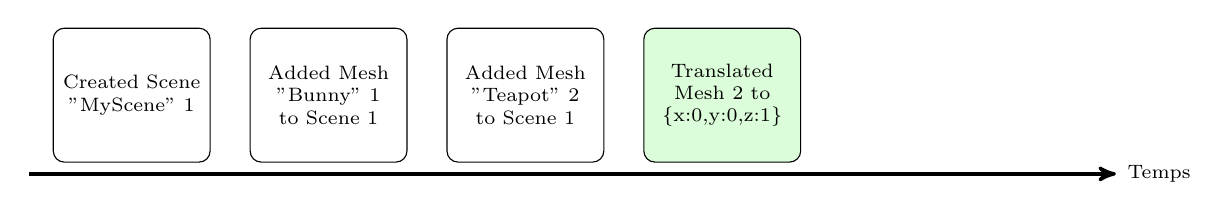
\begin{tikzpicture}[node distance=2.5cm,
		every node/.style={ font=\scriptsize}, align=left,text width=5em,
		text centered,
		axis/.style={very thick, ->, >=stealth',yshift=-1cm}, draw]
		% Specification of nodes (position, etc.)
		
		\node (e1)		[event]          {Created Scene \\"MyScene" 1};
		\node (e2)	  	[event, right of=e1]          {Added Mesh "Bunny" 1 \\to Scene 
		1};
		\node (e3)	  	[event, right of=e2]          {Added Mesh \\"Teapot" 2  \\to 
		Scene 1};
		\node (e4)	  	[eventn, right of=e3]          {Translated \\Mesh 2 to 
		\{x:0,y:0,z:1\}};
		\draw[axis] (-1.3,0)  -- (12.5,0) node(xline)[]{~~~~~~~~~~~Temps};
		
		\end{tikzpicture}
		\caption{Transaction en Event-Sourcing}
		\label{fig:es-transaction}
	\end{figure}
	
	\begin{figure}[!h]
		\centering
		\noindent
		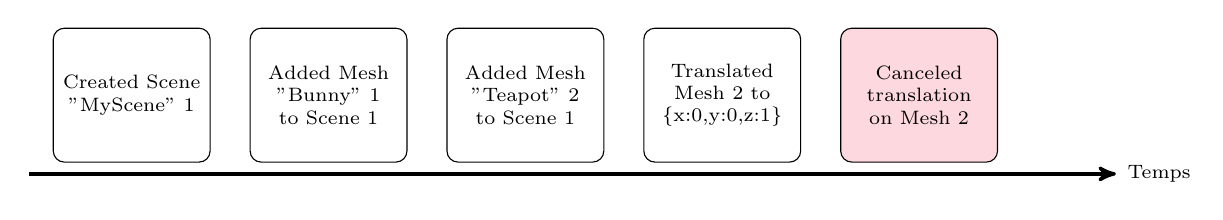
\begin{tikzpicture}[node distance=2.5cm,
		every node/.style={ font=\scriptsize}, align=center,text width=5em,
		text centered,
		axis/.style={very thick, ->, >=stealth',yshift=-1cm}, draw]
		% Specification of nodes (position, etc.)
		
		\node (e1)		[event]          {Created Scene \\"MyScene" 1};
		\node (e2)	  	[event, right of=e1]          {Added Mesh "Bunny" 1 \\to Scene 
		1};
		\node (e3)	  	[event, right of=e2]          {Added Mesh \\"Teapot" 2  \\to 
		Scene 1};
		\node (e4)	  	[event, right of=e3]          {Translated \\Mesh 2 to 
		\{x:0,y:0,z:1\}};
		\node (e5)	  	[eventc, right of=e4]          {Canceled translation on Mesh 2};
		\draw[axis] (-1.3,0)  -- (12.5,0) node(xline)[]{~~~~~~~~~~~Temps};
		\end{tikzpicture}
		\caption{Transaction avec compensation en Event-Sourcing}
		\label{fig:es-transaction-delete}
	\end{figure}
	
	
	\begin{figure}[t]
		\centering
		
		\subfloat[Sans la notion de snapshot]{
			\includegraphics[width=0.4\textwidth]{without-snapshot.eps}
			\label{fig:es-without-snapshot}
		}
		\subfloat[Avec la notion de snapshot]{
			\includegraphics[width=0.4\textwidth]{without-snapshot.eps}
			\label{fig:es-snapshot}
		}
		\caption{Snapshot en Event-Sourcing}
	\end{figure}
	
\subsubsection{Avantages}
L'\gls{ES} peut apporter beaucoup d'avantages à une application, notamment 
lorsque les besoins en traçabilité de l'information sont importants comme dans 
la modélisation collaborative de données 3D.
L'historique du système est accessible tout au long de la vie de l'application ce 
qui implique qu'il est non seulement possible d'accéder à l'état courant du 
système, mais également toutes les actions ayant mené jusqu'à cet état. C'est 
un avantage certain pour les système critiques, les applications d'Informatique 
Décisionnelle (\gls{BI}) ou les applications collaboratives. La pratique la plus 
courante est de proposer un système principal et d'ajouter une multitude de 
sous-systèmes qui enregistrent les différentes métriques (analyse d'un ou 
plusieurs axes, \textit{reporting} sur une propriété) du système principal. Avec 
l'\gls{ES}, il est toujours possible de regarder <<dans le passé>> et récupérer 
les données à partir de ce moment. Par comparaison, les avantages de 
l'\gls{ES} sur l'Active Record sont:
\begin{itemize}
	\item un journal complet de tous les changements d'état,
	\item une traçabilité et un débogage efficace,
	\item de très bonnes performances,
	\item pas de mapping objet-relationnel (ORM)\info{citer fowler's book}.
\end{itemize}

	
\paragraph{Exemple} 
Une revue de projet d'une scène est effectuée dans le cadre d'une application 
collaborative de modélisation 3D en ligne. Le chef de projet remarque qu'un 
objet a subi énormément de modifications par rapport aux autres. Il examine en 
particulier cet objet pour en connaître les causes. Voici deux exemples 
d'observations possibles : 1/ les spécifications ne sont pas assez claires 2/ 
deux collaborateurs sont opposés sur la façon de modifier l'objet. L'origine de 
ces changements identifiée, le chef de projet pourra alors intervenir et clarifier 
le sujet. \improve{style exemple}

\paragraph{Résolution} Avec un système classique, la fonctionnalité doit être 
créée pour enregistrer ce traitement puis être testée et implémentée (dans cet 
exemple, il en faudrait deux). Seulement après, un rapport pourra être délivré. 
Dans un environnement utilisant l'\gls{ES}, tous les évènements existent déjà 
donc les données sont déjà disponibles et ont seulement à être analysées 
(dans 
notre exemples, les informations sont inhérentes aux évènements). De plus, les 
évènements étant stockés depuis le début de la vie de l'application\jp{préciser : 
	début de la vie}, beaucoup plus de données peuvent être analysées. On 
	pourra par 
exemple demander toutes les modifications d'un objet depuis la dernière 
connexion d'un utilisateur pour lui communiquer visuellement les différences par 
rapport à sa dernière visite.



\subsubsection{Inconvénients}
Les performances de l'application peuvent être affectées par l'utilisation de 
l'\gls{ES}. En effet, pour récupérer l'état courant à partir de l'Event Store, il est 
nécessaire de le calculer à partir des évènements reçus.
A chaque évènement créé (et stocké), ce processus sera alourdi car ils ne 
peuvent être supprimés. Plus la pile d'évènements est longue, plus cela prend 
du temps (linéaire). On peut considérer d'une part que l'on a besoin des 
évènements que lorsque qu'une commande est effectuée\info{rehydratation d'un 
agrégat diff avec projection -> eventually consistence (proj = EC /rehy -> 
valides}.\unsure{Dans tous les autres cas l'utilisation de \textit{snapshots} 
permet de contrer proprement ce problème en offrant une forme dénormalisée 
de la donnée.} Un \gls{snapshot} est une capture de l'état de l'agrégat à un 
moment qui correspond à l'empilement d'évènements ayant mené à cet état. En 
créant un \gls{snapshot}, on évite de reconstruire un état à partir du début de la 
vie de l'agrégat; on empile les nouveaux évènements à partir de ce snapshot. 
L'utilisation du \gls{snapshot} est intéressante à partir du moment où la pile 
d'évènements devient plus lourde que le \gls{snapshot} lui-même. Il est donc 
important de bien déterminer la périodicité du déclenchement du \gls{snapshot} 
(temporelle ou selon le nombre d'évènements).

Le parcours des évènements se fait classiquement du premier au dernier 
(\textit{bottom-up}). Si on utilise les \gls{snapshot}, on peut se permettre de les 
parcourir dans l'autre sens (\textit{top-bottom}) jusqu'à trouver un \gls{snapshot} 
puis appliquer tous les évènements qui sont arrivés entre ce \gls{snapshot} et 
l'état courant. Dans le cas où l'on souhaite accéder à des données historiques 
plus anciennes que le dernier \gls{snapshot}, le second parcours fonctionne 
aussi. Cependant, elle doit être évitée pour ne pas créer de dépendance entre 
les \gls{snapshot}. Sans les snapshots le modèle peut encore varier 
<<~librement~>> tant que l'on sait comment lui appliquer un évènement passé. 
Le fait de travailler avec des \gls{snapshot} crée une dépendance des 
snapshots qui doivent intégrer les modifications du domaine. Une solution est 
de recalculer les snapshots quand le domaine est modifié mais cela reste 
coûteux (et à éviter).\info{versionning event -> retro compatibilité}


\subsubsection{Event sourcing vs command sourcing}
Les patrons de conception \gls{CS} et \gls{ES} sont strictement déterministes pour 
avoir une exactitude rigoureuse de ce qui se passe dans le système.

Un évènement représente quelque chose qui est arrivé dans le domaine. Un 
évènement appliqué sur un état, donne un nouvel état. 
La condition pour appliquer un pur déterminisme en \gls{ES} est la fonction 
suivante : \texttt{State $\rightarrow$ Event $\rightarrow$ State}. Cette fonction met 
en correspondance les (mêmes) entrées avec les (mêmes) sorties, on peut se 
reposer dessus pour reconstituer un état à n'important quel moment dans le 
temps. Le déterminisme est appliqué en assurant à l'évènement tous les 
informations lui permettant de faire la transition (i.e. sans effet de bord). 
L'évènement est alors considéré comme une encapsulation de toutes les 
informations pertinentes concernant la transition du système d'un état à l'autre.

Une commande va être déclenchée par l'utilisateur qui veut modifier le domaine. 
Une commande appliquée sur un état va produire un ou plusieurs évènements (qui 
ne sont pas forcément appliqués à l'état courant de l'application par la suite): 
\texttt{State $\rightarrow$ Command $\rightarrow$ Event list}

La différence principale entre un évènement et une commande réside donc dans 
l'\textbf{intention}. D'un point de vue fonctionnel, le \gls{CS} est un patron de 
conception lié à une décision qui produit plusieurs évènements, tandis que 
l'\gls{ES} se contente d'appliquer un changement à l'état courant. De plus, en 
\gls{ES}, l'évènement stocké a été produit par l'agrégat. 
La différenciation majeure des deux patrons de conception s'accentue lors 
l'interaction avec des systèmes externes. L'aspect fonctionnel de l'application de 
changement d'état de l'\gls{ES} al'avantage de permettre de reconstruire l'état sans 
effets de bord car elle ne travaille que sur l'état interne de l'application. 

Historiquement, l'\gls{ES} de Fowler dans ses premières versions ressemblait plus 
à du \gls{CS}. L'évolution de l'\gls{ES} a conduit à revoir ce patron théoriquement 
sous une forme fonctionnelle pure avec l'apparition de base de données comme 
EventStore ou le langage de programmation plus adaptés comme F\#.

Les deux patrons peuvent cohabiter si le \gls{CS} a un cadre d'action bien délimité 
et de les composants de l'architecture ont un couplage lâche afin que seuls les 
évènements produits par les agrégats ne modifient l'état interne de l'application. 


\subsection{Conclusion}



%\chapter{Contributions scientifiques}
%!TEX root = main.tex
\chapter{Contributions scientifiques}
\chaptertable
%\section{Introduction}
Nous avons vu que les \gls{EVC3D} doivent considérer beaucoup de critères pour 
proposer un système réactif, robuste et permettant le passage à l'échelle en 
intégrant les contraintes liées à la gestion de données 3D. La dimension 
collaborative ajoute les problématiques de gestion de données concurrentes.
En s'intéressant d'abord à au rapport des données à la 3D dans le contexte de 
l'assemblage d'objets 3D dans une scène partagée cela permet de 
mieux comprendre les fonctionnalités spécifiques à la 3D (transformations), 
l'historisation des données et leur visualisation. Les ressources nécessaires à la 
collaboration demandent une haute disponibilité et une forte réactivité. Ces 
besoins impliquent de mettre en place une architecture de communication 
répondant aux contraintes fonctionnelles (détection de conflit) et technologiques 
(web).

Ce chapitre présente les contributions scientifiques de cette thèse.
Tout d'abord, on introduit le modèle orienté évènements pour la 
visualisation et la manipulation d'objets 3D dans un environnement web. La 
contribution insiste sur l'intégration de la partie métier de la 3D par l'utilisation de 
patrons de conception (\gls{DDD}, \gls{CQRS}, \gls{ES}) . La réflexion concernant 
le découpage des opérations 3D liées à la manipulation d'objets 3D est expliquée 
dans un premier temps. Dans un second temps, pour procurer plus d'autonomie 
aux utilisateurs, on propose de déporter le patron \gls{CQRS} uniquement sur le 
client afin qu'il soit capable de gérer la partie métier seul. La valeur ajoutée par le 
modèle orienté évènements ne permet pas l'échange entre les utilisateurs bien 
qu'elle soit pensée pour intégrer les aspects métiers de cette dernière. 
C'est pourquoi la seconde contribution s'intéresse à l'architecture de 
communication dans un environnement web. L'architecture hybride proposée 
repose sur une combinaison de l'architecture client-serveur et l'architecture P2P. 
Cela tient du fait que la centralisation de l'information est nécessaire dans un 
contexte industriel et que les propriétés du P2P permettent une haute disponibilité 
des ressources. Cette contribution est découpée en deux parties. La première 
concerne 

%%%%%%% SECTION %%%%%%%
%\section{Modèle évènementiel pour l'intégration du domaine 3D lors de la 
%manipulation d'objets 3D}
%!TEX root = main.tex

%%%%%%% SECTION %%%%%%%
\section{Modèle événementiel pour l'intégration du domaine 3D dans les 
EVC}
\label{sec:modele_event}
%\subsection{Introduction}
La méthodologie orientée événements intègre plusieurs aspects souvent laissés 
de côté dans la littérature concernant le développement des environnements 
virtuels collaboratifs pour la visualisation et la manipulation d'objets 3D. 
Les événements peuvent en effet être utilisés dans le cadre de \gls{CSCW} et 
d'\gls{EVC}, qui ont évolués du simple collecticiel à de plus importantes 
organisations virtuelles comme on peut le retrouver dans des environnements 
scientifiques et d'ingénierie. L'idée de partager des ressources communes pour 
travailler sur un projet commun nécessite des outils propres qui implémentent 
des modèles de collaborations adaptés aux fonctionnalités spécifiques des 
systèmes distribués (forums, chats, tableaux blancs partagés \dots). Ces 
collaborations sont routinières, les motifs de collaboration sont bien connus. Les 
motifs consistent en des segments de collaborations récurrents qui peuvent être 
capturés, encapsulés dans des composants distincts et réutilisés comme des 
solutions pour d'autres problèmes liés à la collaboration. Par exemple, les services 
de sensibilisation permettent de traiter les événements et donner des informations 
à propos du travail collaboratif. En utilisant les événements suivis, les services 
d'analyse fournissent des statistiques à propos des collaborations passées et 
présentes.


Un système orienté événements a l'avantage d'être découplé. Dès 
lors, les données produites lors de la collaboration peuvent facilement être 
réutilisées pour un traitement secondaire comme la sensibilisation aux éléments 
de l'environnement. 
Le découpage de la modélisation logicielle et l'abstraction qu'elle apporte est aussi 
l'occasion de s'intéresser à la façon dont sont générées les données produites par 
les utilisateurs et la façon dont elles sont affichées. 

L'\gls{EP} occupe, dans le champ de l'informatique, une place centrale dans 
beaucoup de systèmes comme l'énergie, la santé, l'environnement, les transports, 
la finance, les services et l'industrie. L'\gls{EP} réunit des méthodes et des outils 
pour filtrer, transformer, et détecter des motifs dans des événements, dans le but 
de réagir à des conditions qui changent, généralement liées à des contraintes de 
temps \cite{Chandy2011}. L'\gls{EP} intègre plusieurs fonctionnalités pour :
\begin{itemize}
	\item obtenir des données à partir de plusieurs sources en temps (quasi) réel ;
	\item agréger et analyser ces données pour détecter des motifs qui indiquent la 
	présence de situations critiques qui nécessitent une réponse ;
	\item déterminer la réponse la plus adaptée à ces situations ;
	\item et surveiller (\textit{monitor}) l'exécution de cette réponse.
\end{itemize}

Le panorama d'applications et de technologies proposé par \cite{Hinze2009} 
permet de définir les termes et les interprétations communes à différents 
domaines se basant sur le paradigme de l'\gls{EP}. 



%L'intégration de la partie métier L'un des aspects principaux a été de 
%combiner tous les aspects reliés aux événements dans le \textit{pipeline} de 
%visualisation et de manipulation d'objets 3D. 


\subsubsection{Constat}

Par nature, une \gls{EDA} est extrêmement peu couplée et 
hautement distribuée. Le créateur de l'événement sait seulement que l'événement 
se produit et n'a aucune idée du traitement que l'événement va subir par 
la suite ou qui cela va concerner. 
C'est pourquoi les \glspl{EDA} sont plus utilisées dans un 
contexte de flux d'information asynchrone. La traçabilité dans ces environnements 
devient alors un enjeu important. Facilitée par l'empreinte laissée par chaque 
événement, elle n'en demeure pas moins complexe selon l'échelle d'évaluation. A 
l'échelle d'un utilisateur, d'un groupe d'utilisateurs, ou de plusieurs groupes, les 
acteurs restent des entités assez homogènes dans le cadre de la modélisation 3D 
collaborative ce qui simplifie la tâche car le contexte et le domaine sont 
connus.



%Il existe différent types de traitement d'événement : simple, en continu, 
%complexe. 
%Ils peuvent être utilisés ensemble dans le cadre d'une même application.
%\begin{itemize}
%\item Traitement d'événement simple. (\textit{simple event processing}). 
%Dans le traitement simple d'événement, un événement notable arrive, initiant 
%une 
%cascade d'actions. Le traitement simple d'événement est généralement utilisé 
%pour 
%orienter un flux temps-réel qui peut prendre un peu de temps, n'entraînant pas de 
%coût sur la partie métier.
%\item Traitement de flux continu d'événement. (\textit{stream event 
%processing}). 
%\item Traitement d'événement complexe. (\textit{complex event 
%processing}). 
%
%\end{itemize}

Le choix de baser la gestion des données sur le patron de conception \gls{CQRS} 
combiné à de l'\gls{ES} repose sur le constat suivant : dans un cadre industriel, le 
besoin de traçabilité de l'information est très important pour suivre l'évolution d'un 
projet par exemple. 
Les \glspl{EDA} reposent le plus souvent sur 
la communication client-serveur pour faciliter la gestion des données dans le 
système distribué. C'est pourquoi l'exploitation du patron de conception 
\gls{CQRS} est traditionnellement développée sur la base d'une architecture client-serveur  (pour récupérer les mises à jour). 
Ce fonctionnement ne permet pas le travail hors ligne.

Côté serveur, le stockage des données est de moins en moins cher, il est possible de stocker beaucoup de données de manière distante notamment 
grâce l'infonuagique. Le serveur a une puissance de calcul 
plus importante (et surtout ajustable).

Côté client, la puissance de calcul des machines sur lesquelles sont installés les 
navigateurs web évolue rapidement (notamment les appareils mobiles comme les 
\textit{smartphones} et les tablettes). Les navigateurs suivent cette tendance en 
puisant dans ces ressources pour effectuer des traitements similaires à ceux que 
l'on trouve traditionnellement côté serveur et pour proposer des fonctionnalités 
avancées telles que le stockage de données sur le client (IndexedDB, 
storageAPI), pour l'affichage 3D (WebGL) et pour la communication en \gls{P2P} 
(\gls{WebRTC}). En déportant ainsi la charge que pourrait subir une architecture 
client-serveur côté client, les échanges réseaux sont limités car ils 
sont très coûteux d'un point de vue énergétique pour les appareils mobiles 
\cite{Koskela2015}. De plus, l'utilisation de la bande passante est onéreuse et 
parfois limitée voire inexistante, il est donc nécessaire de tirer parti de tous les 
appareils participant à la collaboration au lieu de tout faire reposer sur le serveur. 
Chaque appareil participant à la collaboration doit être autonome et le plus 
indépendant possible en termes de ressources (données, réseaux, validation 
experte). 

\paragraph{Contribution}
Pour répondre à cette problématique, je propose un modèle pour la 
transmission des données 3D et collaboratives qui permet de  limiter  le nombre 
de requêtes et la taille des données transmises sans perdre la traçabilité de 
celles-ci. L'idée est de profiter de la puissance du client pour créer une 
architecture assurant l'autonomie de l'utilisateur en cas de déconnexion volontaire 
(travail hors ligne) ou involontaire (coupure). Je garantis ainsi à l'utilisateur 
l'utilisation du système avec un historique performant où chaque connexion est 
l'occasion de mettre à jour le système.\improve{en remettre une couche}


\subsection{Modèle général}
%TODO
%La composition de l'architecture s'est effectuée avec en arrière pensée les lignes 
%directrices  énoncées plus haut\info{ref section} \cite{Xhafa2010}. 
%\todo{reprendre 
%la partie virtualisation dans la partie P2P}
La mise en place d'une \gls{EDA} pour faire de la modélisation 3D engendre des 
avantages pour tous les métiers engagés (utilisateurs, développeurs, analystes 
métier).
\improve{qu'est ce que ça fait la}D'une part la sensibilisation à l'historique des 
données et aux interactions 
inter-utilisateurs est partagée par les collaborateurs et les analystes métier. Les utilisateurs sont mieux informés de l'impact de leurs modifications et ont un aperçu général de l'évolution de la scène. D'autre part, 
la sensibilisation à la distribution des données est une composante 
importante pour les utilisateurs et les développeurs. En effet, la répartition 
de la charge permet de profiter du potentiel computationnel de toutes les parties 
prenantes du réseau. 

Dans 3DEvent, le langage partagé se réfère au domaine de la manipulation 
d'objets 3D mais aussi au domaine de la collaboration. Par exemple le terme de 
maillage peut se référer à la fois au maillage géométrique ou bien au maillage de 
l'architecture réseau, d'où l'importance de définir les différents contextes en amont. 
Notons que le contexte de l'application peut faire varier les frontières d'un 
domaine. Le modèle issu du domaine défini permet de mettre en valeur les 
aspects métiers liés à l'application.

\subsubsection{Spécification des événements dans le framework}
Le framework étant orienté événements, cette section de thèse introduit la 
représentation et 
le vocabulaire utilisé dans la description des événements de 3DEvent. 3DEvent 
reprend la représentation proposée par Tominski \cite{Doktor-ingenieur2006} 
illustrée par la Figure \ref{fig:representation_event}, et adapte ses propriétés pour 
la modélisation 3D collaborative (visualisation et manipulation). 

\begin{figure}[ht]
	\centering
	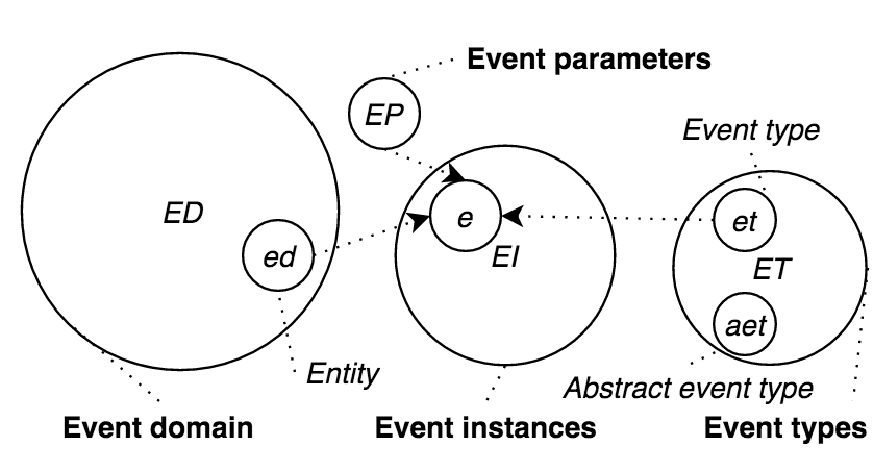
\includegraphics[width=0.7\columnwidth]{eps/event4.eps}
	\caption{Illustration des notions d'événements du domaine, des types 
		d'événements, et des instances d'événements.}
	\label{fig:representation_event}
\end{figure} 

Pour décrire le cadre de référence dans lequel les événements se produisent, la 
notion de domaines d'événements est introduite. Un domaine d'événements 
\textit{ED} (\textit{Event Domain}) contient les événements qui respecte les types 
d'événements qui peuvent être spécifiés. Par analogie avec le \gls{DDD}, cet 
espace correspond au contexte borné (cadre d'action) d'un agrégat. À un agrégat 
sont associés des types d'événements \textit{ET} (\textit{Event Type}) particuliers. 
Un \textit{ET} est utilisé pour exprimer un intérêt concret envers les entités d'un 
\textit{ED}. 
Les événements abstraits \textit{aet} (\textit{abstract event type}) sont 
compatibles avec l'\textit{ED}. 
Une instance d'événement \textit{e} -- ou simplement 
événements -- est composée du triplet \textit{ED}, \textit{ET} et \textit{EP}. 
L'ensemble des toutes les instances d'événements possibles est exprimée par 
\textit{EI}. \textit{EP} (Event Parameters) correspond à l'ensemble des paramètres 
que peut avoir l'\textit{EI}. Ainsi, tous les événements sont liés aux intérêts 
d'un~\textit{ED}. La spécification des événements nécessite de 
s'intéresser à tous les types d'événements qui sont utilisés lors de la manipulation 
et la visualisation d'objets 3D dans un \gls{EVC}. La détection d'événement est un 
processus qui permet de récupérer les instances d'événements d'un \textit{ET} en 
particulier. Cela peut être utilisé pour la visualisation de types particulier par 
exemple. Dans 3DEvent, la spécification des événements est calquée sur les 
comportements observés lors des expérimentations des premiers travaux 
\cite{Desprat2015a, Desprat2015b}. 

Le Tableau \ref{tab:extraitevent} ci-dessous, 
présente les événements de l'agrégat Maillage -- extrait du Tableau 
\ref{tab:events} qui résume les 
différents types d'événements de bases construits à partir du framework et les 
agrégats auxquels ils sont associés. Parmi ces événements, l'événement 
\textit{meshAdded} et \textit{meshDropped} semblent être très proches, voire 
identique quant au résultat que l'utilisateur peut obtenir. Cependant, la sémantique 
liée à chacun permet de différencier l'intention de l'utilisateur. 


\begin{table}[ht]
	\centering
	\caption{événements de pour 
		l'agrégat Maillage (extrait de Tab. \ref{tab:events}) }
	\label{tab:extraitevent}
	\begin{tabular}{lll}
		\toprule
		\textbf{événement}& \textbf{Nommage} & \textbf{Description} \\ \midrule
		%\textbf{Agrégat Maillage}  &                      &             \\ \hline
		Maillage ajouté (*)&     meshAdded                 
		&  \begin{tabular}[c]{@{}l@{}} Un maillage a été ajouté dans\\  la Scène à 
			partir d'une géométrie\\ de la 
			bibliothèque \end{tabular}  \\
		Maillage déposé (*) &     meshDropped               
		&      \begin{tabular}[c]{@{}l@{}} Un maillage a été déposé dans 
			\\l'env. 3D de la Scène à 
			partir \\d'une géométrie de la bibliothèque \end{tabular} \\
		Maillage supprimé & meshRemoved       &        \begin{tabular}[c]{@{}l@{}} 
			Un maillage a été 
			supprimé \\de la Scène \end{tabular}      \\
		Maillage translaté &   meshTranslated  	 &    \begin{tabular}[c]{@{}l@{}} Un 
			maillage a 
			subi une translation \\dans la Scène \end{tabular}              \\
		Maillage pivoté &      meshRotated                &    
		\begin{tabular}[c]{@{}l@{}} Un maillage a 
			subi une rotation \\dans la Scène \end{tabular}           \\
		Maillage mis à l'échelle &  meshScaled           &     
		\begin{tabular}[c]{@{}l@{}} Un maillage a 
			subi une homothétie    \\dans la Scène \end{tabular}    \\ 
		\bottomrule
	\end{tabular}
\end{table}

Ce tableau permet de donner un exemple qui reprend la description qui vient d'être 
présentée. L'\textit{ED} correspond donc au \og système de modélisation 3D 
collaborative\fg{}. Dans ce contexte l'agrégat nommé \og Maillage\fg{} réagit à un 
certain nombre de types d'événements comme \textit{meshAdded}, 
\textit{meshDropped} \dots Les événements typés sont produits par l'agrégat en 
prenant en compte les paramètres nécessaires à leur instanciation. Par exemple, 
la production d'un événement \textit{meshTranslated} prend en paramètre le 
vecteur de translation (x,y,z) et la référence de l'identifiant de la scène à laquelle il 
appartient.


Plus généralement, le domaine est la représentation des objets 3D d'un point de 
vue expert. Les objets du domaine représentent les données liées aux 
manipulations 3D sous une forme abstraite (géométrie, position), indépendamment
des besoins du rendu (lumière, matériau \dots). Le framework intègre un 
générateur d'événements pour faciliter l'implantation de nouveau types 
d'événements au plus proche des besoins des utilisateurs dans une application de 
modélisation 3D collaborative (appuyant la sémantique des manipulations).





\subsection{Adaptation des patrons \gls{ES} et \gls{CQRS}}
%TODO mettre l'image representant le cqrs +  celle de la validation des 
%commandes


La Figure \ref{fig:cqrs-client} montre le déroulement du cycle des opérations du 
modèle au sein de \gls{CQRS}, de l'action utilisateur à la visualisation de son 
résultat. 
Du côté de la partie écriture (partie supérieure -- \textit{write part}), lorsque 
l'utilisateur déclenche une commande à partir de l'interface, la commande et ses 
paramètres sont récupérés et traités par le domaine pour être validés selon les 
règles métiers exprimées par ce dernier. Si la modification est validée, le domaine 
produit ou modifie l'agrégat concerné. Ces modifications sont converties sous 
forme d'événements. Les événements sont ensuite transmis à l'Event Store où ils 
sont stockés 
avant d'être transférés à l'Event Publisher. L'Event Publisher joue le rôle 
d'interface entre la partie écriture et la partie lecture. 
Il est également responsable de la 
publication des événements sur le bus d'événement Event Bus où sont 
accrochées les différentes projections. Les projections sont nourries a partir des 
événements publiés auxquels elles sont abonnées. Enfin, une Vue (composant
inclus dans l'\gls{IU}) récupère les \glspl{DTO}
contenant les mises à jour à partir d'une projection. La mise à jour d'une Vue peut 
se faire de manière passive -- mode \textit{push} -- (ex. : mises à jour liées à la 
visualisation 3D des modifications des collaborateurs en temps réel) ou active -- 
mode \textit{pull} -- (ex : aller sur une autre scène) selon le contexte.

\begin{figure}[h]
	\centering
	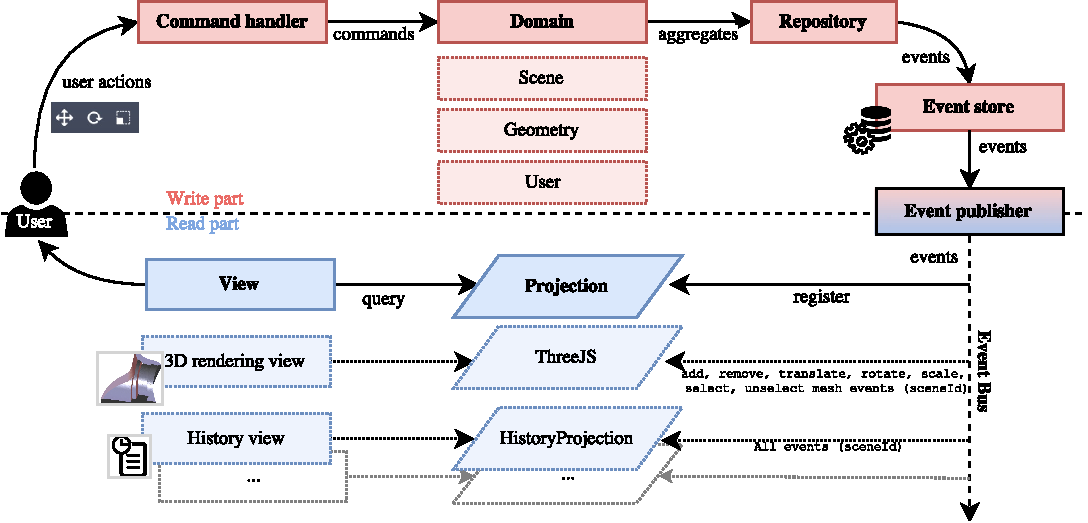
\includegraphics[width=\columnwidth]{eps/cqrs2.pdf}
	\caption[Modèle de l'architecture client dans 3DEvent]{Modèle de l'architecture 
		client dans 3DEvent : la gestion du cycle de vie des données avec 
		\gls{CQRS} 
		et \gls{ES} dans un navigateur web, des actions des utilisateurs à la visualisation 
		en passant par la synchronisation réseau. Issu de \cite{Desprat2017}.}
	\label{fig:cqrs-client}
\end{figure}


Le patron \glsreset{ES}\gls{ES} permet de capturer tous les changements d'état 
d'une application sous la forme d'une séquence d'événements. 
Ces événements sont conservés dans un journal d'événements et peuvent être 
rejoués pour retrouver l'état de l'application. 
Les événements représentent des faits immuables qui sont 
seulement ajoutés au journal les uns après les autres, ce qui permet des taux de 
transaction élevés et une réplication efficace (cf Section 
\ref{sec:es}). Dans 3DEvent, plusieurs composants d'\gls{ES} sont étendus selon 
les applications :

\begin{itemize}
	\item \textbf{Acteur} Un acteur consomme des événements à partir d'un journal 
	d'événements et produit des événements pour le même journal d'événements. 
	L'état interne dérivé à partir des événements consommés est un modèle 
	d'écriture 
	en mémoire (\textit{in-memory}) et contribue à la partie commande (C) du 
	CQRS\info{reference à la section}.
	\item \textbf{Vue} Une vue est un acteur qui ne fait que consommer des 
	événements à 
	partir du journal d'événements. L'état interne dérivé à partir des événements 
	consommés est un modèle de lecture en mémoire et contribue à la partie 
	requête (Q) du CQRS\info{reference à la section}.
	\item \textbf{Producteur} Un producteur est un acteur qui produit des 
	événements à 
	partir 
	du journal d'événements pour mettre à jour la base de données. L'état interne 
	dérivé 
	à partir des événements consommés est un modèle de lecture en mémoire et 
	contribue à la partie requête (Q) du CQRS\info{reference à la section}.
	\item \textbf{Processeur} Un processeur est un acteur qui consomme des 
	événements 
	à 
	partir d'un journal d'événements et produit les événements traités pour un autre 
	journal d'événements. Les processeurs peuvent être utilisés pour connecter les 
	journaux d'événement au traitement des événements.\info{reference à la 
	section}.
\end{itemize}

%\subsubsection{Collaboration événementielle}

\paragraph{Le journal d'événements}

Les événements produits par un des composants présenté ci-dessus
peuvent être consommés par d'autres de ces abstractions s'ils partagent un 
journal d'événements local ou distribué. Un journal d'événements peut 
fonctionner sur un seul site ou être répliqué 
sur plusieurs sites. 
Le site est considéré comme une zone disponible qui accepte 
l'écriture d'un journal d'événements local même s'il est partitionné sur plusieurs 
sites. Les journaux d'événements locaux situés sur plusieurs sites peuvent être 
connectés par le biais d'un journal d'événements dit \og répliqué\fg{} (copié sur une 
autre réplique) qui a pour responsabilité de préserver l'ordre causal des 
événements.
%\todo{dessin des journaux}  
Les sites peuvent être situés à des endroits géographiquement distincts ou sur 
des nœuds à l'intérieur d'une même grappe (\textit{cluster}) ou encore être sur le 
même nœud mais traités séparément selon les zones 
disponibles qui sont nécessaires au fonctionnement de l'application. 
Les Acteurs et les Processeurs écrivent cependant toujours sur leur journal 
d'événements local. 
Les composants peuvent soit collaborer sur un journal d'événements local sur le 
même site, ou au travers d'un journal répliqué sur différents sites.
Il est important de différencier le journal d'événements de la base de données 
(côté serveur) ; la base de données peut ne contenir qu'une partie du journal. 
Une base de données peut également être considérée comme un élément 
complémentaire au journal d'événements, cependant et bien que parfois 
confondus, ils restent bien distincts conceptuellement.
Le journal d'événements commun est la base des échanges pour communiquer 
par le biais d'événements de collaboration. Ce type d'architecture se retrouve dans 
différents cas d'utilisation :
\improve{est ce que cette section est nécessaire?}
\begin{itemize}
	\item \textit{Processus métier distribués.} Les acteurs de différents types 
	utilisent des événements pour communiquer et parvenir à résoudre un problème 
	commun. Bien qu'ils jouent des rôles différents dans le processus métier, ils 
	réagissent à la réception d'événements (programmation réactive) en 
	mettant à jour l'état de l'application et en produisant de nouveaux événements. 
	Cette forme de collaboration est appelée collaboration dirigée par les 
	événements.\improve{ref}
	\item\textit{Réplication d'état d'Acteur.} Les acteurs de même type consomment 
	les événements de chacun pour répliquer l'état interne avec une cohérence 
	causale. Dans 3DEvent, les opérations concurrentes sont autorisées dans 
	l'environnement pour mettre à jour l'état des acteurs répliqués et permettre la 
	résolution interactive de conflit en cas de mises à jour concurrentes et 
	conflictuelles. \improve{miuex 
	expliquer}
	\item \textit{Agrégation d'événement.} Les vues et les producteurs agrègent des 
	événements à partir d'autres composants pour générer des vues spécifiques à 
	l'application.
	La collaboration événementielle apporte de la fiabilité dans la gestion des 
	données dans un système distribué. Par exemple, si un processus distribué 
	échoue à cause d'un problème sur une partie du réseau, le système reprend 
	automatiquement dès les répliques sont à jour.
\end{itemize}

%\paragraph{Bus d'événement}
Les composants souscrivent à leur journal d'événements en s'accrochant au 
\textbf{bus d'événements}.
Les événements nouveaux sont poussés vers les souscripteurs, 
ce qui leur permet de mettre à jour l'état de l'application avec une latence 
minimale. 
Un événement écrit à un endroit est publié de manière fiable aux souscripteurs sur 
ce site et aux souscripteurs des sites distants. 
Par conséquent, les composants qui échangent par le biais d'un 
journal d'événements répliqué communiquent via un bus qui préserve l'ordre causal 
des événements de manière durable et tolérant au partitionnement. De ce fait, les 
services sur les partitions du réseau inter-sites (lien entre les sites) peuvent 
continuer d'écrire des événements localement. La livraison des événements sur 
les sites distants reprend automatiquement lorsque les partitions sont à jour.


Le journal d'événements est répliqué localement et fournit un ordre total des 
événements stockés et appartient à un site. 
Le site est une zone de disponibilité qui héberge un ou plusieurs 
journal d'événements. Les événements d'un journal d'événements sont 
répliqués sur les sites distancts de manière asynchrone. 
Afin de lier des journaux d'événements (localisés sur différents sites) à un journal 
d'événements répliqué, les 
journaux d'événements locaux doivent être accessibles à partir des points 
d'entrées de réplication. De plus, ces points d'entrée doivent être 
connectés entre eux afin de créer un réseau de réplications. 
Un journal d'événements répliqué est représenté par un journal d'événements local 
sur chacun des sites participants.

\info{point d'entrée = network bridge}

Les points d'entrée permettent de gérer un ou plusieurs journaux d'événements. 
Ces journaux sont identifiés pour permettre à la réplication de ne s'intéresser 
qu'aux journaux de même identifiant. 
Les journaux avec différents identifiants sont ainsi isolés les uns des autres et 
leur distribution peut donc varier selon les sites.

Les journaux répliqués fournissent l'ordre causal des événements stockés : l'ordre 
de stockage est le même sur tous les sites, ce qui veut dire que les 
consommateurs qui lisent les événements du journal local vont toujours voir les 
effets avant leurs causes.



\subsection{Cohérence éventuelle en CQRS}


La \gls{CE}, ou \textit{eventual consistency} en anglais, propose dans un système 
distribué contenant plusieurs répliques, d'avoir une coordination lâche entre ces 
répliques. Cela apporte de nombreux avantages en termes de disponibilité, 
tolérance aux fautes et sécurité des données et évite l'intégration de protocoles comme \textit{2 
phase commit} ou de protocoles \textit{Paxos} (consensus) complexifiant les échanges. 
La \gls{CE} introduit l'idée que toutes les répliques se réconcilient au bout d'un 
moment (\textit{forward progression}) pour avoir le même état final. Si le caractère 
vicié d'une information est détecté, le système doit le \og réparer\fg{} pour obtenir 
le bon état. 
\begin{figure} [ht]
	\centering
	\inputTikZ{0.7}{eps/tikz/cap.tex}
	\caption{Théorème CAP et les algorithmes de compromis}
	\label{fig:cap}
\end{figure}
L'ordonnancement des événements durant les mises à jour reste identique lorsque
les événements sont rejoués par la suite car l'ordre issu de l'\gls{ES} est 
déterminée par l'ordonnancement des événements stockés 
localement. Au sein d'une réplique, tous les composants \gls{CQRS} respectent 
cet ordonnancement. L’ordre de stockage des événements répliqués sur des sites 
distincts est cohérent sont ordonnés de manière causale \cite{Lamport1978} : les 
événements liés causalement ont le même ordre sur tous les sites alors que les 
événements concurrents peuvent avoir un ordre différent. Cette propriété est 
importante pour obtenir une cohérence causale forte dans une application qui 
respecte le théorème \gls{CAP} (Figure \ref{fig:cap}).  \blockquote[]{	\textit{The 
largest single 
benefit about 
CQRS is when 
		you start running into 
		problems 
		with the CAP theorem}}{
	\cite{Young2010}
}.
Young justifie ensuite que le lien entre \gls{CAP} et \gls{CQRS} est plus ténu qu'il 
n'y paraît. Même si \gls{CQRS} ne permet pas d'éviter le dilemme de \gls{CAP}, le 
fait que \gls{CQRS} découpe le système en petites parties permet d'ajuster la 
cohérence séparément.

Dans \gls{CQRS}, l'interaction avec plusieurs agents (utilisateurs, services) est 
découplée et subit un traitement réparti 
dont résulte la cohérence éventuelle de l'application. 
Dans la conception d'interaction pour l'interface, la synchronicité peut varier en 
fonction certains contextes. 
Les interactions asynchrones rajoutent souvent des étapes qui polluent l'interface.  
Par exemple, dans le cas de l'interaction suivante : \texttt{soumission de 
formulaire -> envoi asynchrone -> message de confirmation}, si l'utilisateur attend 
que la soumission soit une requête qui peut probablement échouer, alors 
l'asynchronisme se justifie pour être capable de fournir une explication à 
l'utilisateur en cas d'erreur. 
La probabilité d'échec peut être réduite en pré-validant la commande. Si personne 
d'autre que 
l'utilisateur ne travaille sur l'agrégat, la probabilité d'échec est quasi-nulle. De ce fait, 
l'asynchronicité rajoute une interaction inutile au flux dans le cas où peu de gens 
travaillent sur la même instance d'agrégat.
Par exemple, il est intéressant de rendre l'exécution d'une 
commande synchrone et la mise à jour de la vue asynchrone. Les modèles de 
cohérence sont des décisions liées au métier car ils ont un impact direct sur 
l'expérience utilisateur. 


Dans ce modèle événementiel, la partie Commande permet de limiter l'introduction 
de données impropres dans le système via différentes mécanismes. Chaque 
commande issue de l'\gls{IU} entraîne la génération d'un ou plusieurs événements. 
Ces événements sont considérés 
comme \og soumis\fg{} (\textit{uncommitted}) mais pas encore <<~publiés~>> 
(\textit{committed}) par le système.
Une commande peut-être rejetée pour différentes raisons. Ces raisons sont 
exprimées par différentes phases de validation de la commande.
Une première validation se fait en amont du déclenchement de l'\gls{IU} avec par 
exemple une vérification de type des paramètres passés à la commande.

%Linéaire (strong consistency)
%one version replace another -- one parent and one children in the sequence
%each version is immutable 
%each version has an identity
%each new version is a replacement of the previous (earlier)
%directed acyclic graph (eventual consistency)
%each version may have one or more parent
%each parent may have one or more parent
%each parent may have children with different parents
%each version is immutable
%each version has an identity
%
%each version may be viewed as one of many replacement version for its parents
%
%version are immutable and (should) have immutable names


%\begin{algorithm}[caption="titi"]
%	
%    saveEvents(itemId:string, events:EventMessage[], expectedVersion:number) 
%{\\
%    	var eventDescriptors:EventDescriptor[] = 
%this.eventDescriptorsByAggregate[itemId];\\
%    	if (!eventDescriptors) {\\
%    		eventDescriptors = this.eventDescriptorsByAggregate[itemId] = [];\\
%    	} else if (eventDescriptors.length > 0 \&\& 
%eventDescriptors[eventDescriptors.length\\ - 1].version != expectedVersion \&\& 
%expectedVersion != -1) {\\
%    	throw new Error("ConcurrencyException");\\
%    }
%    var i = expectedVersion;\\
%    events.forEach((event:EventMessage) => {\\
%    	i++;\\
%    	event.version = i;\\
%    	var eventDescriptor = {id: event.AggregateId(), version: i, eventData: 
%event};\\
%    	eventDescriptors.push(eventDescriptor);\\
%    	this.\_publisher.publish(event);\\
%    	this.\_network.publishEvent(event);\\
%    });
%}
%\end{algorithm}
\subsection{Potentielles applications et autres utilisations}
La conception et l'implémentation d'une plateforme comme 3DEvent qui est 
asynchrone, distribuée et orientée événements peut 
être appliquée à différents champs.
\begin{description}
	\item[GIT-like app] Les solutions pour faire de la gestion de version, comme 
	MeshGit~\cite{Denning2013} par exemple qui fait du
	\textit{diff and merge} de maillages polygonaux pour des données 3D, 
	sont rarement implémentées (a fortiori en 
	temps-réel) sur des plateformes web à cause du coût et de la complexité que 
	cela peut apporter dans des architectures traditionnelles. 3DEvent peut 
	reconstruire n'importe quel état antérieur grâce à son architecture orientée 
	événements et indiquer les différences entre deux états.%\todo{acyclic graph}
	
	\item[Scenarii et \textit{path recording}] Pour des jeux sérieux, l'infographie 
	3D ou des études d'ergonomie, cette fonctionnalité est particulièrement 
	pertinente. Le \gls{framework} peut proposer une comparaison entre deux traces 
	laissées par un ou plusieurs utilisateurs. Dans le cas où les utilisateurs ont la 
	même tâche à réaliser, il est facile de faire la différence entre deux réalisations 
	pour comparer, analyser et montrer les résultats	pour des raisons 
	pédagogiques ou pour relever des habitudes (de travail) par exemple. Dans 
	l'exemple du jeu sérieux, il est possible de comparer la trace utilisateur à la trace experte 
	et permettre de rejouer le même scénario plusieurs fois facilement pour 
	observer l'évolution. Ce type de fonctionnalité est intrinsèque à 3DEvent. 
	
	\item[Traçage utilisateur et \textit{crowdsouring}] 3DEvent peut se révéler être 
	un bon outil pour enregistrer la trace d'un utilisateur lorsqu'il navigue dans la 
	scène. L'enregistrement du chemin de la caméra et des actions de l'utilisateur 
	sous la forme d'événements sont des informations 
	"issues de la foule" (\textit{crowdsouring}). En utilisant un processus 
	d'apprentissage, il est possible de proposer de meilleurs chemins, repérer des 
	points d'intérêt, ou même proposer des résumés de scène générés à partir des 
	traces des collaborateurs (que s'est-il passé depuis la dernière connexion du 
	collaborateur X ?).
	\item[Audit et outils de surveillance de données 3D] L'\gls{ES} fournit un 
	mécanisme 
	d'audit intégré qui assure la cohérence des données transactionnelles. Utiliser 
	ce mécanisme pour faire un audit ou surveiller en temps réel l'activité de 
	l'application peut fournir une meilleure compréhension du travail d'équipe ainsi 
	que l'évolution de la conception. Cela peut permettre de repérer (avec du 
	\gls{CEP}) et corriger certaines fonctionnalités afin d'améliorer l'ergonomie de 
	l'application. Par exemple, si un événement est anormalement représenté dans 
	le journal des événements, il sera possible de lever une alerte facilement.
\end{description}
%\begin{figure}[htb]
%	\centering
%	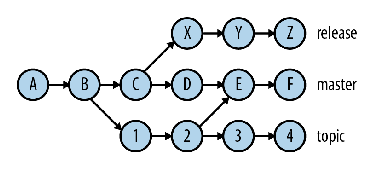
\includegraphics[width=0.3\columnwidth]{gitgraph}
%	\caption{Exemple d'arbre de commits Git}
%	\label{fig:git}
%\end{figure}
\subsection{Bilan}

Le modèle orienté événement pour la modélisation 3D collaborative présenté dans 
cette section intègre les besoins métiers par différents aspects. Le suivi des 
directives liées au \gls{DDD} permet de mieux cerner les règles 
métiers pour les intégrer dans \gls{CQRS}. 

La description de la typologie des 
événements manipulés insiste sur le compartimentage des objets métiers. La 
modélisation 3D collaborative est minutieusement étudiée pour en dégager les quatre 
agrégats fondamentaux (la scène, le maillage, la géométrie et l'utilisateur) et les 
types d'événements qui leurs sont associés. Cette étape introduit des différences 
fines sur les événements qui sont produits à partir d'un agrégat. 
Cet aspect est notamment intéressant pour l'observation et la surveillance du 
contenu des sessions collaboratives développés en Section 
\ref{sec:flexviz}. \todo{attention garder le bon endroit}
Les composants du patron \gls{CQRS} favorisent le découplage de l'application 
pour obtenir une gestion de la cohérence plus fine. 

La partie \gls{ES} s'intéresse à la sauvegarde des événements dans un journal 
d'événement, et notamment dans le cas des applications distribuées en proposant 
un mécanisme de synchronisation pour détecter les conflits. La fonction principale 
de cette partie est de permettre de recréer un état de l'application cohérent en 
intégrant implicitement une gestion de version des événements.

Ce modèle introduit le cadre de travail pour utilisateur expert en manipulation 3D, il 
peut être facilement adapté pour différents types d'applications et étendu à 
d'autres utilisations. 
Pour mettre en avant l'expertise de chacun et profiter de 
toutes les ressources apportées par un utilisateur, une communication efficace de 
ces événements pour la collaboration doit désormais être établie entre les 
collaborateurs.

%%%%%%% SECTION %%%%%%%
%\section{Architecture de communication hybride}

%%%%%%% SECTION %%%%%%%
\section{Architecture de communication hybride}

%\subsection{Introduction}

Dans la section précédente, l'introduction du modèle orienté événements 
s'intéresse principalement à ce qui se passe au sein d'un seul client. 
Or la collaboration passe par la mise en relation des différents collaborateurs, mais aussi par  
l'échange des données nécessaires à la collaboration (données de connexion, 
mises à jour de la scène, sensibilisation\dots)
Afin de pouvoir proposer un \gls{SEC} adapté aux besoins de l'édition de scènes 
3D, plusieurs types de granularité sont à distinguer : 
\begin{itemize}
	\item une granularité fine pour l'édition massive ;
	\item une granularité liée aux spécificités de la modélisation \gls{3D} ;
	\item et une granularité reposant sur des technologies web (réseau, interface, 
	interaction \gls{3D}).
\end{itemize}

Les systèmes \gls{P2P} qui sont orientés événements consistent en plusieurs 
n\oe uds interconnectés dont les fonctions et l'exécution des tâches sont
similaires. Les pairs partagent directement leurs ressources (contenu, CPU, 
stockage, bande passante) sans nécessiter de serveur central. A la place, les 
pairs coopèrent au moyen d'événements qui prennent la forme de messages lorsqu'ils
se les échangent. Les systèmes \gls{P2P} sont capables de s'adapter aux 
dysfonctionnements et à la dynamicité des pairs, tout en maintenant des 
performances acceptables. Les systèmes \gls{P2P} sont généralement utilisés 
comme soutien aux services de l'application pour la communication et la 
collaboration, le calcul distribué, la distribution de contenus et pour les services 
d'intergiciel comme le routage et la localisation, ou encore l'anonymat et la confidentialité.

\paragraph{Constat} Les \glspl{SEC} ont connu un fort développement avec 
l'intérêt 
croissant 
pour le \gls{P2P} dans les années 2000. 
La base théorique des \glspl{SEC} s'appuie sur les propriétés de 
convergence, préservation de la causalité et préservation de l'intention du modèle 
\acrshort{CCI} \cite{Sun1998}. 
La plupart des travaux liés aux \glspl{SEC} \gls{P2P} s'intéressent à 
l'édition collaborative massive de documents textuels dont les propriétés 
de commutativité sont plus faciles à gérer (insertion / suppression) en 
comparaison à celles concernant la \gls{3D} (multiplication de matrices de 
rotation). La génération de conflits en \gls{3D} peut vite devenir incontrôlable. Il est 
donc nécessaire de mettre en place des mécanismes de détection de 
conflits et de maintenir une cohérence au cours des sessions de 
collaboration. 





%\gls{WebRTC} est une technologie qui fournit aux navigateurs 
%\textit{destkop} et mobiles la possibilité de communiquer en temps-réel 
%(cf \ref{sec:webrtc} via une collection de standards, 
%protocoles et \glspl{API} JavaScript. 
%L'un des atouts de cette technologie est de permettre de façon simple et 
%sans module d'extension la capture d'un flux audio et / ou vidéo (ex : 
%applications de VoIP), ainsi que l'échange de données arbitraires entre 
%navigateurs sans nécessiter d'intermédiaires (ex : partage de fichiers en 
%\gls{P2P}).
%Techniquement, \gls{WebRTC} supporte un canal temps-réel 
%bidirectionnel pour l'échange de données. Contrairement à 
%\gls{WebSocket}, qui est basé sur \gls{TCP}, \gls{WebRTC} repose sur 
%\acrshort{UDP} en intégrant une pile de plusieurs protocoles (Figure 
%\ref{fig:protocolstack}) qui lui offre des fonctionnalités similaires (fiabilité, 
%ordonnancement, sécurité). 

%TODO parler chargeet distribution


\paragraph{Contribution}
La mise en place d'une architecture de communication 
hybride permet de concilier à la 
fois les avantages d'une architecture client-serveur et ceux du \gls{P2P}, en évitant 
certains désavantages occasionnés dans ces derniers (engorgement du serveur, 
pair seul sur le réseau\dots). 
Le terme \og hybride\fg{} invoque un compromis entre la 
centralisation de l'information nécessaire à la prise de décision globale et 
la décentralisation des échanges utile à l'amélioration du partage de 
contenus \gls{3D} à l'échelle locale. 
En agissant sur ces deux échelles, la granularité de la collaboration est plus fine. 
Par exemple, le passage à l'échelle est facilité par la présence de 
ressources locales et la coordination des utilisateurs se fait à une échelle 
globale, ce qui permet également l'accès à une source de vérité 
centralisée (base de données) et commune.
Dans le contexte des \glspl{EVC3D}, le but 
est d'obtenir une architecture de communication : 

\begin{itemize}
	\item entièrement basée web ; 
	\item robuste face à l'évolution du nombre de collaborateurs ; 
	\item efficace en termes d'accès et de distribution de la donnée ; 
	\item et qui s'adapte à l'échelle selon les besoins de la collaboration.
\end{itemize}


Tous les travaux liés à cette thèse, 
\cite{Desprat2015a,Desprat2015b,Desprat2016} et \cite{Desprat2017}, s'appuient sur une 
architecture de communication hybride tripartite (Figure \ref{fig:hybrid}) pour 
faire de la modélisation \gls{3D} collaborative : serveur, persistance 
et les pairs\footnote{Les pairs sont appelés \og Clients\fg{} dans les premiers 
travaux}. 

Les contributions portées par Desprat et al. dans 
\cite{Desprat2015a,Desprat2015b} 
s'appuient sur des pairs ayant un rôle simple et proposent une transmission des 
mises à jour en tant que différentiel d'état. Les conflits lors d'opérations 
concurrentes sont évités grâce à un mécanisme de verrouillage. 
Plus tard, dans \cite{Desprat2016}, les auteurs mettent en place le modèle 
orienté événements qui impose l'évolution, au niveau réseau, du protocole 
de transmission (celui-ci reposant sur 
des notifications d'événements et la gestion des flux d'agrégat). 
Plus récemment, dans \cite{Desprat2017}, est apparue la distinction entre 
les deux rôles parmi les pairs : la 
partie serveur se compose désormais de pairs qui ont un rôle de vérification 
de la cohérence et de relais des données dans la couche \gls{P2P}. Cette 
contribution intervient dans le but d'encourager la résilience du système et la 
vitesse de dissémination des informations dans le réseau, en favorisant la prompte 
détection de conflits (source de vérité plus proche des pairs producteurs). 
Cette extension repose sur la présence d'un journal d'événements partagé et 
répliqué sur les pairs participants à la collaboration.

\begin{figure}[h!]
	\centering
	\includegraphics[width=0.7\columnwidth]{eps/hybrid5.eps}
	\caption{Architecture hybride tripartite : serveur, persistance 
		et les pairs.}
	\label{fig:hybrid}
\end{figure}

Cette section décrit le modèle d'architecture mis en 
place pour gérer la transmission de contenu entre les différents clients 
qui participent à l'édition collaborative d'un espace de travail \gls{3D} partagé. 
Les différents protocoles de transmission, issus des travaux sus-nommés, 
sont présentés. Ils montrent ainsi l'évolution de l'architecture de communication de 
sa version naïve à la version étendue, plus proche des considérations métiers et 
offrant plus de liberté dans la création grâce la mise en place d'un système inspiré 
des \glspl{CRDT}.
 
Les différents éléments constitutifs d'un pair sont détaillés avant la présentation 
des deux types de pairs rencontrés dans l'architecture.
Sont expliqués ensuite les mécanismes de mise en relation de 
ces composants pour que les différents participants d'une session 
collaborative puissent communiquer de manière transparente, cohérente et 
résiliente.

%TODO reprendre pour partie implantation
%Les travaux présentés s'inscrivent dans un contexte où les besoins 
%d'interopérabilité et de standardisation sont élevés pour permettre à des 
%utilisateurs de prendre le système rapidement en main sans installer autre chose 
%qu'un navigateur. 


\subsection{Éléments constitutifs d'un pair}
Un réseau \gls{P2P} pour le calcul ou la transmission d’information est un modèle 
d’architecture qui permet de distribuer les tâches et la charge de travail entre 
différents pairs. Chaque pair ou \og n\oe ud\fg{} est à la fois client et serveur, ce 
qui implique que les pairs sont à la fois fournisseurs et consommateurs de 
ressources contrairement au traditionnel modèle client-serveur où la production et 
la consommation sont séparées. Les pairs mettent directement à disposition des 
autres participants du réseau une partie de leurs ressources (espace de stockage, 
CPU, GPU) sans nécessiter une coordination centrale par un serveur. En cela, les 
pairs ont (en général) les mêmes privilèges et participent de façon équipotentielle 
dans l’application.

Dans un réseau \gls{P2P}, chaque pair est considéré comme un système à part 
entière qui contient ses propres problématiques d'implémentation. Avant de 
présenter la contribution liée à l'intergiciel dans 3DEvent\todo{ref section}, il est 
nécessaire 
d'introduire les composants et les fonctions clés qui constituent un pair du point de 
vue strictement réseau en 
présentant une vue minimaliste d'un pair dédié au partage de contenu 
\cite[p.135-136]{Buford2009}. Les 
fonctions sont divisées en trois :
\begin{itemize}
	\item la couche de routage et d'échange de messages ;
	\item la recherche et le stockage de contenu ;
	\item ainsi que la configuration et sélection du rôle du pair.
\end{itemize}


\begin{figure}[ht]
	\centering
	\inputTikZ{0.9}{eps/tikz/middleware/middleware}
	\caption{Composants de chaque pair dans 3DEvent (point de vue réseau)}
	\label{fig:middleware}
\end{figure}


Chaque pair générique fournit de base une \gls{API} pour les fonctions d'échange 
de messages et de recherche. 
L'\gls{API} de recherche est principalement en lien avec le 
gestionnaire d'instances qui se charge de la recherche, mais il est possible de se 
connecter à des pairs via d'autres pairs si le serveur est absent ou pour renforcer 
le maillage.
L'élément responsable de la couche de routage et d'échange de messages permet 
à chaque pair de maintenir un état de connexion avec ses voisins dans la couche 
; maintenir cet état inclut la découverte de voisins et la maintenance  à jour des 
états des voisins.
Un pair possède un mécanisme d'amorçage (\textit{bootstrap}) qui permet de 
localiser les autres pairs qui lui permettront de rejoindre la couche \gls{P2P}. Les 
étapes pour rejoindre ou quitter la couche sont proposées par le protocole 
d'établissement de connexion 
(cf signaling mecanism\todo{ref section signaling}).
La couche applicative permet d'échanger des messages avec les autres pairs 
dans le réseau en utilisant l'\gls{API} réseau, et les messages reçus peuvent être 
transférés à leur destination en utilisant la fonction de transfert de messages. 

Le contenu partagé est stocké localement pour pouvoir être accessible par d'autres 
pairs, ainsi que l'interface de l'application du pair courant. Le contenu doit être 
organisé pour la recherche d'informations afin de fournir une indexation et une 
interface de requête. 
L'espace de stockage pour les données partagées va correspondre aux différents 
états des agrégats \cite{Desprat2015a,Desprat2015b} ou au journal d'événements 
\cite{Desprat2016,Desprat2017}.


La dernière fonction concerne la manière dont le pair auto-organise, à la fois, ses 
ressources locales et son rôle dans le réseau. Le pair détermine les 
ressources du système et du réseau disponibles et peut surveiller les 
changements éventuels régulièrement.
Le pair a connaissance du rôle qui lui est attribué à sa création dans le réseau. Les 
rôles des pairs (super pair, relai, producteur\dots) dépendent de 
capacités comme les ressources du système et du réseau. Le rôle induit les 
capacités et la configuration de chaque pair, i.e. un pair actif est configuré 
uniquement pour produire, stocker et relayer les données tandis qu'un pair passif ne fait que stocker et relayer les données. La stabilité du pair peut être indiquée par son niveau de 
\textit{churn} (dynamicité : rejoindre et quitter un réseau) par exemple. 
La Figure \ref{fig:middleware} peut être affinée en fonction du type de 
réseaux et d'applications. Chaque pair comprend un protocole pour la gestion
de sessions (ex: REST API) et pour l'échange de données (ex: RTCDataChannels)  
pour pouvoir participer à la collaboration.



Les architectures de communication des contributions se divisent en deux parties, 
chacune correspondant au paradigme qu'elles utilisent respectivement : état ou 
événement. Selon le paradigme auquel elles font référence, elles peuvent 
être décrites par plusieurs critères:
\todo{revoir}
\begin{description}
	\item[Spécificité des composants de l'architecture] Les pairs sont la base de la 
	dissémination de l'information. La partie serveur 
	centralise les données liées à la persistance long  terme et
	décentralise la réplication des données à court terme. Cela évite au 
	serveur 
	d'être le point central des échanges en déchargeant les canaux passant par le 
	serveur.
	\item [Gestion de la session] 
	La gestion de la session suit le cycle de vie des pairs au sein du réseau 
	lorsqu'ils participent à une session collaborative. 
	Pour intégrer le réseau \gls{P2P} et participer à l'édition d'une scène \gls{3D} de 
	manière collaborative, les clients passent par les étapes suivantes :
		\begin{enumerate}
		\item Phase de \textit{signaling}
		\label{phase1signaling}
		\begin{enumerate}
			\item Signification de la présence auprès du serveur de \textit{signaling}
			\item Récupération de la liste des identifiants des pairs auxquels se 
			connecter
			\item Création d'une connexion \gls{P2P} avec les autres pairs
			\item Souscription aux flux
			
		\end{enumerate}
		\item Phase de synchronisation
		\label{phase2sync}
		\begin{enumerate}
			\item Requête des données manquantes
			\item Récupération des données manquantes
			\item Ré-ordonnancement des messages reçus
			\item Maintien de la cohérence (détection de conflit)
		\end{enumerate}
		
		\item Phase de génération de nouvelles données valides 
		\label{phase3gen}
		\begin{enumerate}
			\item Publication des données aux voisins
		\end{enumerate}
		
		\item Phase d'abandon
		\label{phase4quit}
		\begin{enumerate}
			\item Notification aux voisins 
			\item Fermeture des canaux
		\end{enumerate}
	\end{enumerate}
	
	Ces quatre phases sont distinctes même si, lorsqu'un pair initialise ou rejoint 
	une 
	session collaborative (séquence d'initialisation), les phases 
	\ref{phase1signaling}, \ref{phase2sync} et \ref{phase3gen} s'enchainent pour 
	ce pair. Durant la session collaborative, les phases \ref{phase2sync} et 
	\ref{phase3gen} s'alternent. La phase \ref{phase4quit} se produit lorsque qu'un 
	client quitte une scène de manière volontaire (changement de scène, fermeture 
	de l'onglet du navigateur) ou involontaire (fausse manipulation, navigateur en 
	panne, coupure internet) signifiant la fin de la session collaborative.
	
	\item [Gestion du stockage et structure des données] 
	Le stockage peut prendre plusieurs formes : \textit{in-memory}, stockage local, 
	disque dur\dots selon le type de stockage adapté et disponible. 
	Dans l'architecture hybride, il existe deux niveaux de stockage : la persistence 
	long-terme, distante -- la base de données -- et la persistence court-terme, 
	locale -- le navigateur.
	Le serveur assure, d'une part, la centralisation du stockage à long-terme, et 
	d'autre part, la mise en relation des différents clients.
	\item [Gestion de la synchronisation et de la cohérence (détection des conflits)] 
	Il existe différentes possibilités de synchronisation des pairs. 
	
	L'édition concurrente lors de la collaboration peut être gérée de différentes 
	manières, selon si elle est plutôt pessimiste ou optimiste lors de la réplication 
	des 
	données (voir Section \ref{sec:concurrence}). L'intégration d'une solution ou 
	l'autre 
	a de lourds impacts sur l'expérience utilisateur (fonctionnalités, interface 
	utilisateur) et la gestion de la cohérence dans le réseau \gls{P2P}.  
	
	\item [Protocole d'échange]
	La couche \gls{P2P} fournit une dissémination rapide de l'information et 
	\todo{finir}
\end{description}


%
%\subsection{Architecture de communication \og orientée états\fg{}}
%\label{sec:comm_state}

\subsection{Architecture hybride \og orientée états\fg{}}
\label{sec:comm_state}

Les premiers travaux liés à cette thèse \cite{Desprat2015a,Desprat2015b} se sont 
intéressés principalement à la mise en place de l'architecture de communication 
en basant les structures de données sur des états (plutôt que des événements). 
Cette section décrit les choix faits lors de la modélisation de l'architecture \og 
orientée état\fg{}, pour le stockage et le transfert par exemple, en lien fort avec les 
technologies web sous-jacentes. 

%  well for web distributed sys- tems even if mobile devices should have limited 
%  perfor- mance due to back and forth requests that are energy consuming.
%  
\subsubsection{Spécificité des composants de l'architecture}
Le système présenté repose sur une architecture \acrshort{REST} 
(\acrlong{REST}) concernant les échanges clients-serveur. Cette architecture 
permet de séparer les responsabilités entre le client et le serveur en séparant 
l'\gls{IU} du stockage. \gls{REST} propose une interface uniforme. Cela implique 
que chaque ressource est identifiée et manipulable par des représentations définies 
(modification, suppression). 

Chaque pair correspond a un client (navigateur web) qui contient l'intergiciel 
\gls{P2P} offrant des fonctionnalités limitées, l'interface utilisateur contenant 
l'environnement \gls{3D} et un espace de stockage reposant local (IndexedDB).

La persistance long terme est une base de données NoSQL. Ce type de bases de 
données a tendance à être optimisée en lecture (grâce à un 
langage de requête dédié) et permet d'éviter les 
structures rigides. Cette flexibilité est utile lors du stockage des modèles \gls{3D} 
et 
encourage la conservation d'autres métadonnées (ex: relations entre les différents 
objets) pour faciliter la traçabilité. 
Avec une base de données centralisée, le système possède une source de 
données fiable et autoritaire qui permet à un utilisateur de récupérer le bon contenu 
quand il revient sur une scène. La totalité du document, contenant la scène, est 
envoyé à l'utilisateur lorsqu'il y accède.


\subsubsection{Gestion du stockage et structure de données}

Avec une base de données NoSQL utilisant des schémas dynamiques, les 
données sont stockées sous forme de document. Chaque document est 
auto-descriptif et peut contenir des valeurs qui s'imbriquent sous la forme d'une 
structure en arbre hiérarchique. Une collection consiste à grouper des documents, 
équivalent, dans une base de données relationnelle, à la notion de table. La base de 
données contient deux types de collections : les scènes et les géométries. Une 
collection de scènes contient des scènes qui sont décrites par leur identifiant et 
les méta-données de l'espace virtuel \gls{3D}, ainsi que la liste des contributeurs et 
la 
liste des maillages. Cette liste correspond à une association entre un identifiant de 
maillage, les méta-données de l'objet et l'identifiant d'une géométrie existante. 
Les géométries sont, quant à elles, stockées avec leur identifiant propre et l'objet 
3D complet donné sous le format \gls{JSON}.

Sur chaque pair, il existe un stockage relationnel pour 
chaque objet de la base de donnée récupérée. Cela permet au client de faire des 
requêtes directement dans son espace local si besoin, par exemple en ajoutant un maillage. 
C'est également une source pour transférer ses modifications aux autres clients.
Les navigateurs permettent désormais de stocker des quantités de données 
importantes localement avec une durée de vie illimitée. 
Les paramètres des opérations fondamentales effectuées sur la base de données 
(\gls{CRUD}) sur les collections sont très bien supportés par les requêtes 
\gls{REST}.



%
%We propose to auto connect users on a scene with a We- bRTC connection. As 
%each user send their ID to the database at their arrival, they also retrieve those 
%which where already present on the scene. We are able to cre- ate a full mesh 
%topology network in order to make them communicate the updates.
%
%Even if we have a full mesh topology, the P2P message layer is more similar 
%the 
%star topology. Indeed, the Fig- ure 2 shows the path of a sent message 
%operation 
%on the connection and it is only sent to the one degree neigh- bors of the original 
%broadcaster (the “B” node on the Figure 2).
%
%
%We choose to keep reliable and in order delivery for now. The RTCDataChannel 
%API supports many data types (strings, binary types: Blob, ArrayBuffer. . . ). 
%These types are helpful in a 3D multi user environment to broadcast messages 
%including the objets and their transformations. We tried to limit the amount of 
%data 
%by sending only relevant information but there is actually no particular 
%optimization. The channel can be over- feed when an object is imported then 
%pushed through the network.
%

\subsubsection{Gestion de la synchronisation et de la cohérence}
\label{sec:synchronisation-client-serveur}

Les travaux \cite{Desprat2015a} et \cite{Desprat2015b} présentent une version 
naïve du processus de synchronisation. La cohérence est garantie par un système 
de verrouillage des objets. Cela évite notamment les sélections concurrentes et par 
conséquent les éditions concurrentes. 
Lors de la récupération de la scène, elle est considérée comme cohérente. 
Ensuite, le choix d'avoir des connexions \gls{P2P} ordonnées et fiables, ainsi 
qu'un maillage de pair complet, implique que toute donnée envoyée par un pair est 
forcément reçue par les autres. 
L'échange des mises à jour entre le client (persistance à court terme) et la 
base de données (à long terme) leur permet de se synchroniser dans un premier 
temps. La base de données peut également servir en cas de conflits importants ; 
elle sert de référence.

Lors de la connexion d'un nouveau client, a lieu la synchronisation des deux 
systèmes de persistance pour obtenir les mises à jour : 

\begin{enumerate}
	\item depuis le client, où l'on distingue trois cas :
	\begin{enumerate}
		\item travail "\textit{offline}" (hors ligne) : l'utilisateur a travaillé hors ligne et 
		doit maintenant publier "en ligne" son travail. Les mises à jour sont publiées 
		sur la base de données ; le serveur vérifie si aucun conflit ne survient puis 
		fusionne (\textit{merge}) les nouvelles entrées avec l'existant; 
		
		\item travail "\textit{serverless}" (en collaboration avec entre pairs sans le 
		serveur) : dans le cas où le serveur est absent, les clients peuvent continuer 
		de créer en collaborant. Ces données n'étant stockées que sur le client, il est 
		nécessaire de les transmettre à la base de données dès qu'une connexion 
		est possible. 
		
		\item travail "\textit{online}" (en collaboration entre pairs comprenant la partie
		serveur) : le client systématiquement ses 
		nouvelles modifications pour qu'elles soient intégrées à la base de données.
	\end{enumerate}
	\item depuis la base de données :
	Le client reçoit toutes les nouvelles mises à jour de la scène depuis la dernière 
	fois qu'il s'est connecté. Cela peut également inclure des mises à jour qui sont 
	en conflit avec ce qu'il y a dans son propre espace de stockage, qu'il lui faut 
	donc modifier.
	Dans le cas où un seul utilisateur est connecté, la base de données est la 
	seule source disponible pour la mise à jour du client. 
\end{enumerate}


Le fait de synchroniser un client avec une base de données NoSQL dès que cela 
est possible permet de supporter les connexions intermittentes comme pour les 
appareils mobiles dans cette architecture ; cette approche est connue sous le nom 
de \og\textit{offline first}\fg{} \cite{Gadea2016}.
\subsubsection{Topologie et protocole d'échange}
Cette architecture est basée sur une topologie de maillage complet (\textit{full 
mesh topology}) pour le réseau \gls{P2P}.
Les échanges se font donc à deux niveaux: entre les pairs, ainsi qu'entre chaque 
pair et la base de données. Pour le premier niveau, la couche réseau \gls{P2P} est 
assez 
naïve dans le sens où les connexions sont considérées comme fiables et 
ordonnées ; le client n'a alors qu'à publier toutes les modifications qu'il effectue et 
les envoyer à tous les clients (auxquels il est nécessairement connecté).
Les pairs échangent des différentiels d'état sur les objets. Ces messages ne 
contiennent pas d'information sémantique sur le type d'action effectuée par chaque 
utilisateur. 

\subsubsection{Discussion sur les architectures de 
communication orientée \og états\fg{}}

La base de données centralisée est beaucoup sollicitée lors des sessions 
collaboratives, ce qui peut mener à une surcharge similaire aux architectures 
uniquement client-serveur. 
En combinant client-serveur et \gls{P2P}, la charge aurait dû être réduite et 
transférée aux autres pairs, notamment lors de la phase de récupération d'une 
nouvelle scène qui repose entièrement sur le serveur. 
Chaque pair assume la responsabilité dans l'envoi de ses modifications à tous les 
autres pairs. Cette tâche ne profite pas du réseau \gls{P2P} de manière optimale 
car la topologie ne profite pas de la fonction relais des pairs. Cela pourrait alléger  
la distribution dans la couche \gls{P2P} et responsabiliser un peu plus les pairs 
pour faciliter le passage à l'échelle.
En effet, la topologie en maillage complet limite le passage à l'échelle car le 
nombre de connexions va croître de manière exponentielle. 

Par ailleurs, les requêtes \gls{CRUD} ne sont pas très expressives concernant le 
métier. 
Aucune vérification n'est donc effectuée sur la validité des données transmises 
dans cette architecture. De plus, il peut arriver, du fait de latences réseaux que les 
modifications des différents utilisateurs s'entrelacent à l'arrivée et ne rendent pas 
l'intention de l'utilisateur. Cela peut mener à des dé-synchronisations fortes.

Concernant la gestion de la concurrence, l'utilisation d'une solution pessimiste 
dans un environnement \gls{P2P} peut parfois mener à des inter-blocages si un 
utilisateur quitte la scène sans avoir relâché l'objet, c'est à dire sans en avoir 
informé la base de données et les autres 
utilisateurs. 
Même si l'application peut prendre le relais et permettre la relâche du 
verrou au bout d'un certain temps, l'expérience utilisateur peut être dégradée 
pendant cette période.
Le maintien de la cohérence est garanti dans ce modèle si l'on 
considère un environnement où la fréquence des modifications n'est pas très 
élevée, et que tous les clients communiquent leur horloge locale pour établir un 
référentiel de temps concernant les mises à jour. 

Enfin, le transfert par différentiel d'état utilisé pour réduire la taille des 
données liées au changement d'état des objets lors de la transmission des 
données peut varier grandement selon le type de changement 
effectué, rendant peu prévisible la charge des canaux de communication. 
%
%Some issues remain in RTCDataChannel API : the com- patibility and 
%interoperability is still not complete be- tween browsers6, some browsers (like 
%Chrome) im- pose a send limit (about 6MB) for the data transmitting through 
%DataConnections and the security of the com- munication is still vulnerable7. 
%The 
%system overview (Figure 4) illustrates the communication architecture topology 
%between the peer clients and server (plus sig- naling).



%\subsection{De l'état à l'événement}
%\label{sec:statetoevent}

\subsection{De l'état à l'événement}
\label{sec:statetoevent}
Afin d'intégrer la notion d'historique dans une application web, plusieurs indicateurs 
sont nécessaires (version, granularité de l'historisation, type et taille des données 
manipulées). Cette section décrit le processus pour passer d'un système basé 
états à un système basé évènements dans l'intérêt de réduire la somme des 
données transmises sans perdre d'information concernant la logique métier.
\paragraph{Description des variables}
Une scène $S$ contient l'ensemble des $n$ objets $x$ ($S =\{x_0,x_1,...,x_n\}$). 
Chaque élément de $S$ est associé à une taille calculée comme la somme des 
modifications $m$ selon la version $v$. 

Pour tout objet $x$ appartenant à la scène $S$ on associe une taille $w \in 
\mathbb{R}$. $w$ correspond à la taille totale des données transmises pour 
modifier l'objet à chaque version $v$ ($v$=0 correspond à la taille de l'objet à l'état 
original, i.e. l'\gls{EventStore} est vide). La taille totale de la scène, notée $Sw$, 
correspond à sommer la taille de tous ses objets (équation \ref{eq:sw}). Toutes les 
variables évoquées sont exprimées en octet pour avoir des termes avec des 
unités homogènes.

\begin{equation}
\label{eq:sw}
\text{Taille d'une scène $S$ : } S_w= \sum_{i=0}^{n}w_i
\end{equation}


\paragraph{Transmission par état}
Dans un système où à chaque modification on transmet l'état complet (équation 
\ref{eq:complet}), la taille des éléments transmis correspond à la somme de tous 
les états par lesquels l'objet est passé. Cette valeur va augmenter par paliers de 
tailles relativement équivalentes.
La transmission par état permet d'avoir un historique grâce à une sauvegarde 
chronologique. Cependant elle est lourde voire redondante et n'offre pas 
d'information sur l'intention de l'utilisateur (quelle opération a permis d'arriver à cet 
état?).

\begin{equation}
\label{eq:complet}
\text{Par état : } w_i = \sum_{v=0}^{n}state_{v}
\end{equation}


\paragraph{Transmission par différentiel d'état}
\label{par:diff}
Dans un système où l'on transmet un différentiel d'état (équation 
\ref{eq:différentiel}), la différence entre deux états peut être difficile à exprimer 
\info{cf meshhisto} car il s'agit d'un objet 3D dont les informations, stockées dans 
un fichier, ne sont pas linéaires. Le différentiel peut beaucoup varier jusqu'à 
atteindre une taille proche de l'état actuel si une transformation génère beaucoup 
de modifications par rapport à l'état précédent. A contrario, une modification sur la 
position d'un objet peut être très légère. La fonction représentant la taille des 
ressources transmises augmentera par palier avec au pire les propriétés de la 
proposition précédente (équation \ref{eq:complet}). Le différentiel d'état permet 
d'alléger la transmission par rapport à la proposition précédente, ne contenant 
cependant pas d'information sémantique sur ce qui est transmis et les opérations 
qui ont conduit à l'état d'un objet 3D de la scène.

\begin{equation}
\label{eq:différentiel}
\text{Par différentiel d'état : } w_i = state_0 + \sum_{v=1}^{n}(\underbrace{state_{v} 
- state_{v-1}}_{differential})
\end{equation}

\paragraph{Transmission par évènement}
La transmission par évènement (équation \ref{eq:evenement}) repose sur le 
principe du différentiel d'état ($differential$) exprimé ci-dessus (équation 
\ref{eq:différentiel}) en ajoutant la notion de type d'évènement ($eventType$). Le 
type d'un évènement indique le nom de la transformation à appliquer pour passer 
d'un état à l'autre. Un évènement contient par nature une sémantique <<métier>> 
associée à chaque opération qui donne des indications sur l'intention de 
l'utilisateur. 

\begin{equation}
\label{eq:evenement}
\text{Par évènement : } w_i= state_0 + \sum_{v=1}^{n}(\underbrace{eventType + 
differential}_{event}) 
\end{equation}

Dans un \gls{EVC3D}, il y a des évènements concernant à la fois la manipulation 
3D, la navigation et les éléments se rapportant à la collaboration (par exemple: 
prendre le point de vue d'un collaborateur). La taille d'un évènement est variable 
(comme un différentiel d'état) avec un minimum contenant le type d'évènement 
($eventType$) dû à sa structure type/paramètres. Cette proposition est un peu 
plus lourde à transmettre que la précédente mais ajoute une valeur sémantique à 
l'historique.



%\subsection{Architecture de communication \og orientée événements\fg{}}
%\label{sec:comm_event}

\subsection{Architecture de communication hybride \og orientée 
événements\fg{}}
\label{sec:comm_event}

Cette architecture est une combinaison des contributions présentées dans 
\cite{Desprat2016,Desprat2017} : elle repose sur les éléments du 
framework orienté événements (Section \todo{ref modele event}) qui sont également 
en relation avec la couche réseau (Figure \ref{fig:archievent}).
\begin{figure}[ht]
	\centering
	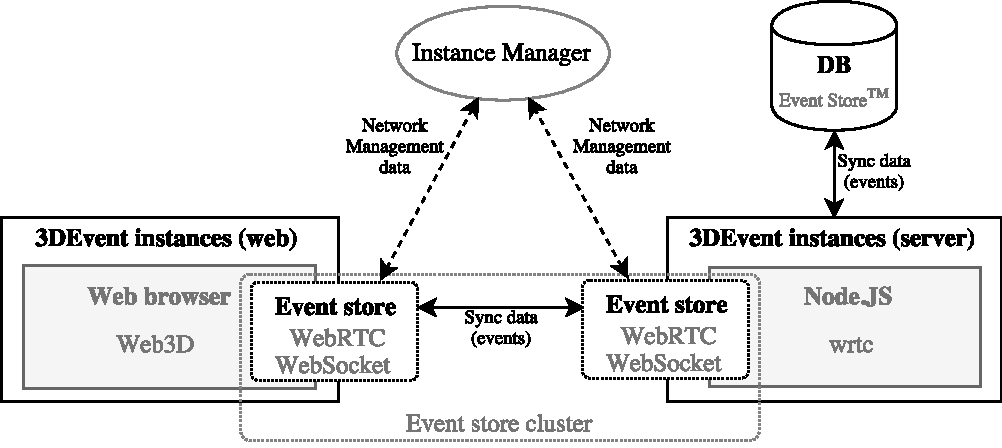
\includegraphics[width=\columnwidth]{eps/archi.pdf}
	\caption{Architecture de communication \og orientée événements\fg{}}
	\label{fig:archievent}
\end{figure}

\subsubsection{Spécificité des composants de l'architecture}
L'Event Store est un composant clé dans le traitement des événements. Présent 
sur chaque pair, il prend en entrée des événements de deux natures : ceux qu'il a 
générés via la partie commande (internes) et ceux reçus via le réseau 
principalement (externes). 
L'Event Store produit en sortie des événements dits \og 
cohérents\fg{} qui peuvent être publiés par la suite sur l'Event Publisher.
Un Event Store est composé de deux types d'éléments : 
\begin{itemize}
	\item l'\gls{ESM} qui gère les flux d'événements : structure de données 
	présente dans chaque Event Store qui doit permettre l'accès en lecture et en 
	écriture des agrégats qu'elle contient. 
	Un \gls{ESM} contient des flux d'événements ordonnés temporellement 
	pour chaque agrégat géré ;
	\item les \glspl{NB} qui servent de connecteurs réseaux : responsables de la 
	gestion d'une connexion \gls{P2P}, i.e. gère le flux de données entrant et 
	sortant vers chaque pair auquel ils sont reliés.
\end{itemize}

La Figure \ref{fig:archievent} montre des pairs (appelés instances) de différentes 
natures :
\begin{itemize}
	\item Instance Web :  produit, stocke et relaie des événements aux autres 
	instances.
	\item Instance Serveur : stocke et relaie des événements aux autres instances 
	et à la base de données. 
\end{itemize}

En plus de servir de relais comme une Instance Serveur, une Instance Web est 
productrice d'événements. C'est en général le type d'instance par lequel un 
utilisateur accédera à l'application. Les Instances Serveurs, en comparaison avec 
l'architecture présentée précédemment, sont des \og serveurs\fg{} qui participent 
directement à la couche réseau. En cela, ils aident à la dissémination des données 
et peuvent rapidement être montés pour garantir une disponibilité des données 
auprès des autres instances (notamment en cas de panne).
Toutes les instances sont coordonnées par l'\gls{IM} qui est responsable de mettre 
les pairs en relation. Il est notamment le serveur responsable dans le mécanisme 
de \textit{signalling}. 

L'ensemble des Event Stores forme une grappe (\textit{cluster}) qui gère le 
journal d'événements partagé de manière répartie entre toutes les instances.
\subsubsection{Gestion du stockage}
\paragraph{Local avec l'\gls{ESM}}
Lorsque l'Event Store reçoit de nouveaux événements, l'\gls{ESM} crée ou 
récupère le flux d'événements associé à l'agrégat dans un premier temps. Puis, il 
stocke l'événement à la suite de ceux présents dans le flux de l'agrégat.

\paragraph{Long-terme et distant avec une base de données fonctionnelle}
Dans un contexte industriel de collaboration, l'information doit être disponible sur le 
long-terme, facilement accessible par l'entreprise. La persistance à 
long-terme stocke le journal d'événements qui est la 
source de vérité de l'application. Elle peut également stocker des projections 
prédéfinies, calculées à la volée ou encore des \textit{snapshots} de l'application.

Sur la base du modèle orienté événements, les données à stocker sont les 
événements. Ils sont immuables et 
constituent des données purement fonctionnelles\todo{voir section \gls{ES} vs CS}.
L'utilisation d'une base de données fonctionnelle permet de se reposer sur 
l'immuabilité des événements.
L'argument souvent opposé à l'utilisation de telles bases est le coût de l'espace de 
stockage. Or le coût de la redondance et de la non localité du traitement des 
données, a chuté au cours de ces dernières années. 
Une base de données dont les données muent -- i.e où chaque donnée peut être 
modifiée à n'importe quel moment -- ne permet pas de conserver l'historique des 
modifications (ex : \textit{Active Record}). Dans une base de données dite 
fonctionnelle, les données stockées sont immuables -- i.e. elles ne peuventt être modifiée \textit{a posteriori} et fait seulement référence à 
d'autres données immuables. Une telle base de données est \og \textit{une interface vers 
des \textit{snapshots} versionnés}\fg{} \cite{Meric2012}.

Dans le cas de l'\gls{ES}, les événements sont considérés comme des deltas 
(avec quelques métadonnées supplémentaires) sur les agrégats. C'est donc sous 
leur forme originale qu'ils sont stockés. Cela évite également les transformations 
de données (et la perte d'information ou l'ajout de complexité) qui sont nécessaires 
dans les \glspl{ORM}, en lecture et en écriture.

\subsubsection{Gestion de la synchronisation et de la cohérence}
Dans \cite{Desprat2017} lorsqu'un pair initialise ou rejoint la séquence pour 
rejoindre une session collaborative, il évolue pour se synchroniser et intégrer les 
nouveaux événements à son journal.
La Figure \ref{fig:connexionpairs} représente la séquence d'actions nécessaire à 
une instance 3DEvent ($idA$) pour rejoindre le réseau contenant déjà d'autres 
instances 3DEvent. L'action \textit{join} est exécutée lorsqu'un utilisateur envoie 
ses informations de connexion sur un portail de connexion (à partir d'une instance 
web) ou lorsqu'une instance serveur est lancée. Cette action ajoute le nouveau 
pair à la liste des pairs présents sur le réseau. Cette liste est gérée par le 
gestionnaire d'instance, qui la retourne au pair pour lui indiquer les pairs 
avec lesquels il doit se connecter.
Pour chaque pair $idB$ de la liste retournée $ids$, $idA$ utilise le mécanisme de 
signalisation (offre/demande). Le mécanisme est déclenché par l'instanciation d'un 
\gls{NB} dans l'Event Store de $idA$ puis celui de $idB$. Afin de resynchroniser 
les deux pairs (après cette série d'échanges asynchrones), $idA$ et $idB$ 
s'échangent des méta-données sur la situation respective de leurs \gls{ESM} 
afin de se synchroniser\todo{(see refernece sync mechanism}.

\begin{figure}[h]
	\noindent
	\centering
	\includegraphics[width=\columnwidth]{connection.eps}
	\caption{Protocole de connexion au réseau d'instance 3DEvent}
	\label{fig:connexionpairs}
\end{figure}

\paragraph{Cohérence d'un agrégat}
Les événements sont considérés comme \og cohérents\fg{}  lorsqu'il n'y a pas 
d'erreur de cohérence dans l'agrégat, i.e. lorsqu'il n'y a pas de doublon dans les 
numéros de versions et qu'ils sont bien ordonnés. Lorsqu'un \gls{ESM} ne 
rencontre pas de problème de cohérence, alors le 
dernier index correspond au numéro de version de l'agrégat. 

Lorsque l'Event Store reçoit un événement interne, l'\gls{ESM} récupère (ou crée) 
le flux d'événements associés à l'agrégat référencé par l'événement. 
La cohérence de la version est alors vérifiée en comparant la version attendue 
(exposée dans les méta-données de l'événement) et la version actuelle de 
l'agrégat. 
Si les deux numéros de version sont identiques, l'événement est ajouté à la fin du 
tableau du flux pour être stocké dans l'\gls{ESM}, sinon une exception est levée. 
La gestion des exceptions est expliquée dans\todo{détails exception}. 

\paragraph{Mécanisme de gestion de version}
3DEvent intègre une procédure de gestion de version dans l'\gls{EventStore} afin 
de gérer au mieux la cohérence des données (voir Section \todo{ref section}). 
Pour être cohérent, l'agrégat concerné par ces 
événements doit produire une nouvelle version, sans être en conflit avec la 
précédente. En passant la version attendue $v_a$ au gestionnaire de conflits, on 
est à même de la comparer avec la version courante $v_c$. Il existe deux cas où 
un conflit est levé~: 
\begin{enumerate}[label=\alph*)]
	\item \label{i:vi} La version $v_a$ correspond à la valeur d'initialisation
	\item \label{i:vdiff} La version $v_a$ est différente de la version $v_c$
\end{enumerate}
Dans \ref{i:vi}, après une action, la version initiale de l'agrégat ne 
peut être la même. Cet item peut sembler évident mais il est important de le noter 
car il dépend entièrement de la valeur initiale choisie pour les agrégats du 
\gls{framework} (on peut commencer à n'importe quelle valeur -- -1, 0\ldots).
\todo{parler de b), et redite par rapport a au dessus}



\subsubsection{Topologie et Protocole d'échange}
L'architecture hybride orientée \og événements\fg{} tire profit de la présence des 
Instances Serveur pour réduire la responsabilité des pairs producteurs (Instances 
Web) dans la distribution des données. En effet, les Instances Serveur qui 
participent au réseau permettent de proposer plus de points de distribution de 
données directement reliés à la base de données. De ce fait, la politique de 
connectivité entre les pairs peut être réduite, le réseau a une topologie maillée 
partiellement (\textit{partial mesh topology}). 


\subsubsection{Gestion de la cohérence}



Pour chaque événement sauvegarder, l’Event Store publie (push) l’événement sur 
le bus (Event Publisher). Cette mécanique est expliquée dans l'algorithme 
\ref{algo:saveEvent}. \todo{finir explications}

\begin{algorithm} % enter the algorithm environment
	\caption{Sauvegarde d'événements d'un agrégat dans l'Event Store} % 
	%give the algorithm a caption
	\label{algo:saveEvent} % and a label for \ref{} commands later in the document
	\begin{algorithmic} % enter the algorithmic environment
		\Require aggregateId : string, uncommitedEvents : eventMsg[ ], 
		version : number
		%\Ensure $y = x^n$
		\State $expectedVersion \Leftarrow version$
		\For{$eventMsg $ \textbf{in} $uncommitedEvents$}	
		\State{$newMsg \Leftarrow \{type : eventMsg.typeEvt, data : eventMsg, 
			streamId : aggregateId\}$}
		\State{$publish(aggregateId, newMsg, expectedVersion++)$}
		\EndFor
	\end{algorithmic}
\end{algorithm}
\todo{parler de cet algo}
\begin{algorithm} % enter the algorithm environment
	\caption{Ajout d'un événement dans l'Event Store} % 
	%give the algorithm a caption
	\label{algo:addevent} % and a label for \ref{} commands later in the document
	\begin{algorithmic} % enter the algorithmic environment
		\Require streamId: string, event: EventStoreEvent, version: number
		\Ensure event
		\State $stream \Leftarrow streams.getOrCreate(streamId);$
		\If{$ stream.has(version)$}
		\State $throwExceptionVersion(stream,version)$
		\EndIf
		\State $stream.data.set(version,event) $
	\end{algorithmic}
\end{algorithm}

\todo{categories: type d’agregat
	c’est un flux liés a une categorie (exemple geometries) tous les events liés à la 
	categorie.}

\todo{metadata phase sync permet a un nouveau noeud de recup toutes les info 
	manquantes et de les demander de maniere repartie a tous les noeuds}



\begin{algorithm} % enter the algorithm environment
	\caption{Synchronisation d'un n\oe ud de l'Event Store partagé} % 
	%give the algorithm a caption
	\label{algo:synchnode} % and a label for \ref{} commands later in the document
	\begin{algorithmic} % enter the algorithmic environment
		\Require $node : ClusterNode$
		\Ensure $nodeState == synchronized$
		\State $nodeMetadata \Leftarrow node.getMetadata()$
		\If{$nodeMetadata != \{\} $}
		\State $streamsToSync \Leftarrow metadata.getDiff(nodeMetadata)$
		\While{$streamsToSync > 0$}
		\State $streamToSync \Leftarrow streamsToSync.pop()$
		\State $events \Leftarrow  node.getEvents(streamToSync)$
		\If{$! streamToSync.has(version)$}
		\For {$event$ \textbf{in} $events$}
		\State $processEvent(event.streamName, event, 
		event.version)$
		\EndFor 
		\EndIf
		\State $streamsToSync \Leftarrow metadata.getDiff(nodeMetadata)$
		\EndWhile
		\EndIf
		\State $node.endSync()$
	\end{algorithmic}
\end{algorithm}

L'algorithme \ref{algo:synchnode} décrit la synchronisation d'un n\oe ud avec un 
autre n\oe ud dans l'Event Store partagé. Le n\oe ud courant demande le 
différentiel (\textit{diff}) entre ses flux et ceux du n\oe ud $node$ pour 
connaître quels sont les flux à synchroniser. Si un n\oe ud possède les données 
demandée il les envoie. Si le n\oe ud courant reàoit à nouveau les mêmes 
données, elles sont ignorées par le système.






\subsubsection{Discussion des problématiques liées à une architecture de 
communication orientée \og événements\fg{}}
Architecture réactive à l'attrition. Tous les éléments qui participent à la gestion de 
données, actifs dans la distribution ou producteurs de données, sont au même 
niveau. Le réseau \gls{P2P} est renforcé par la présence de pairs destinés à 
faire le relais dans la distribution des données. 

La gestion de la cohérence \todo{finir}


%
%\subsubsection{Gestion de la cohérence}
%
%
%\subsubsection{Respect de la causalité}
%\subsubsection{Convergence des répliques}
%\subsubsection{Préservation de l'intention}

%\paragraph{Connexion des pairs en début de session}







\subsection{Comparaison des deux architectures}

% Please add the following required packages to your document preamble:
% \usepackage{booktabs}
\begin{table}[h]
\centering
\caption{Récapitulatif des deux approches d'architecture de communication}
\label{ta:recap-approche}
\begin{tabular}{@{}lll@{}}
\toprule
\textbf{Critère}    & 
\textbf{HybridEvent}                                                                                      & 
\textbf{HybridState}                                                                                      \\ 
\midrule
Type stockage pair  & Fonctionnel 
(event)                                                                                       & 
Relationnel                                                                                               \\
Type BDD            & Fonctionnel 
(event)                                                                                       & NoSQL (Doc. 
JSON)                                                                                         \\
Cohérence           & 
Éventuelle                                                                                                & 
Forte                                                                                                     \\
Synchronisation     & 
Push-pull                                                                                                 & 
Push                                                                                                      \\
Gestion de conflit  & 
Flexible                                                                                               & 
Verrouillage des objets                                                                                   \\
Robustesse          & \begin{tabular}[c]{@{}l@{}}Plusieurs pairs sont liés \\ au 
serveur BDD : \\ disponibilité ++\end{tabular} & 
\begin{tabular}[c]{@{}l@{}}Lourde charge pour le \\ serveur lié à la BDD:\\ 
disponibilité - -\end{tabular} \\
Connectivité pair   & One-to-many 
(policy)                                                                                      & 
One-to-all                                                                                                \\
Passage à l'échelle & 
Oui                                                                                                       & 
Faible                                                                                                    \\
Orientée métier     & 
Oui                                                                                                       & 
Non                                                                                                       \\
Transmission        & Notification 
événement                                                                                    & Diff. 
état                                                                                                \\
Topologie Maillage  & 
Partiel                                                                                                   & 
Complet                                                                                                   \\
Type données        & 
Évènement                                                                                                 & 
État                                                                                                      \\
Type requêtes       & Projection / 
DTO                                                                                          & CRUD / 
REST                                                                                               \\
Historique des données         & 
Oui                                                                                                       & 
Non                                                                                                       \\
Défaire / Refaire   & Oui 
(compensation)                                                                                        & 
\begin{tabular}[c]{@{}l@{}}Oui (annulation commande \\avec effets de 
bord)\end{tabular}                \\ \bottomrule
\end{tabular}
\end{table}


\section{Conclusion du chapitre}
Dans ce chapitre nous avons vu les différents composants de l'architecture de 
communication pour réalisation d'un \gls{EVC3D}. En mettant en avant la 
technologie WebRTC, nous avons montré qu'il était possible de réaliser une 
architecture qui respecte les standards du web et l'interopérabilité nécessaire à ce 
type d'environnement. La mise en place d'une architecture décentralisée dans un 
environnement distribué permet de mettre à contribution tous les acteurs de la 
collaboration. De ce fait, l'accessibilité des ressources est renforcée par la 
présence de nombreuses unités présentes sur le réseaux. Cela permet à la fois 
une récupération du contenu rapidement et octroie une autonomie certaine aux 
contributeurs. 


%\chapter{Implantation}
%!TEX root = main.tex

\chapter{Implantation}
\chaptertable

\section{Introduction} 
Cette section présente l'implantation de 3DEvent, la plateforme web de 
manipulation et visualisation collaborative d'objets 3D réalisée à partir du modèle 
présenté dans le chapitre précédent.

La première partie s'intéresse à l'intégration 
du framework pour proposer une application d'assemblage d'objets 3D. La 
présentation commence avec la description de l'\gls{IU} et des fonctionnalités 
proposées dont le principe de sélection fantôme et le système de visualisation 
flexible reposant sur le système de projection du modèle orienté événements. 

La seconde présente l'implémentation de l'architecture de communication avec les 
différentes implémentation des acteurs du système, les politiques de connexion et 
l'intergiciel \gls{P2P} qui permettent l'échange de données entre les collaborateurs.

Enfin, la troisième section récapitule et discute les choix techniques pour 
l'interface utilisateur et la partie réseau qui ont été fait dans l'implémentation.


\section{3DEvent : Plateforme web de manipulation collaborative d'objets 3D}
Dans le chapitre précédent une des contribution présentée correspond au 
modèle orienté événements : le \gls{framework} 3DEvent. 
Son implémentation prend la forme d'une application web qui intègre un éditeur 
pour la visualisation et la manipulation d'objets 3D de manière collaborative (aussi 
appelée \og application 3DEvent\fg{}).

%\chapter{Implantation}
%\section{3DEvent : Plateforme web de manipulation et visualisation 
%	collaborative 
%	d'objets 3D}
\subsection{Éditeur 3DEvent}
L'intérêt de proposer une application web se 
retrouve principalement dans 
l'accessibilité qu'elle propose. En effet, n'importe 
quel terminal muni d'un 
navigateur web peut y accéder, ce qui la rend distribuée et multi-plateforme. 
Les fonctionnalités graphiques proposées par WebGL sont un peu réduites par 
rapport à celles d'OpenGL dont l'\gls{API} évolue plus vite et propose plus de 
flexibilité et d'optimisations. Cependant, les performances graphique restent très 
correctes car le navigateur est quand même capable d'utiliser les processeurs 
graphiques du terminal (GPU) pour les calculs et rendus \gls{3D}.

Pour faire le lien entre le modèle et l'expérimentation, l'implantation du modèle a 
pris la forme d'un éditeur pour la modélisation \gls{3D} haut niveau permettant de 
visualiser et manipuler des objets \gls{3D} de manière collaborative dans un 
environnement web (aussi 
appelée \og application 3DEvent\fg{}). Au sein de la plateforme, les interactions 
possibles sont : 
\begin{description}
	
	\item[Visualiser, naviguer, utiliser les outils de transformation] L'utilisateur peut, 
	com\-me dans un environnement \gls{3D} classique, interagir avec la vue en 
	utilisant 
	la souris (survol, clic) et en bougeant la caméra (déplacements). Il peut 
	utiliser les commandes clavier et souris pour effectuer des opérations de 
	translation, de rotation et d'homothétie de trois manières différentes: directement dans le \textit{viewport}, via le 
	menu ou via la console du navigateur.
	\item[Charger des modèles \gls{3D}] L'éditeur gère la plupart des formats de 
	fichier 
	3D \info{ref [Bou12]}(OBJ, PLY, DAE, glTF\ldots)
	\item[Changement de référentiel] La modification des coordonnées de 
	réfé\-ren\-ces (local/global)  pour les différentes transformations possibles
	\item[Grid snapping] Cette fonctionnalité permet d'aligner les modèles avec la 
	grille avec un effet de magnétisme sur les intersection de la grille.
	\item[Changement de point de vue] L'utilisateur peut à tout moment passer de 
	son point de vue à celui d'un autre utilisateur. Le choix d'implanter ce type de 
	fonctionnalité s'inscrit dans la perspective de sensibilisation de l'utilisateur au 
	travail de ses collaborateurs. Ainsi, lors de la session, le fait de prendre le 
	point de vue d'un collaborateur est une manière de 
	comprendre son fonctionnement et d'imaginer ses 
	perspectives de conception à travers son angle de caméra qu'il a choisi.
\end{description}



\subsection{Interface utilisateur orientée tâche}

Dans le but de proposer une \gls{IU} proche des fonctionnalités métiers liées à la 
modélisation \gls{3D}, l'éditeur possède une interface orientée \og tâche\fg{}, en 
comparaison avec des \gls{IU} \gls{CRUD}. En effet, les \gls{IU} \gls{CRUD} 
réduisent la sémantique métier du domaine d'application à la création, la lecture, la 
mise à jour et la suppression, omettant toutes les subtilités que peuvent dégager 
ces actions en perdant l'intention de l'utilisateur dès le niveau de l'interface. Une 
interface orientée tâche a tendance à s'attarder sur toutes les nuances que le 
domaine possède en caractérisant chaque action sans subir d'effet de 
simplification. Cette proximité avec le métier permet de calquer directement 
l'interface du modèle événementiel sur l'\gls{IU} et de guider l'utilisateur dans ses 
activités. L'utilisabilité, qualité de l'expérience utilisateur fournit par un système 
pour réaliser une tâche, est alors maximisée en terme d'efficacité, d'efficience et 
de satisfaction. 
Ce type d'\gls{IHM} s'organise autour de cas d'utilisation. Cela permet, 
d'une part, de présenter clairement les 
actions (\og ajouter une géométrie à la 
bibliothèque à partir d'un fichier\fg{} plutôt que \og téléverser un fichier\fg{}) : 
l'intention est clairement définie. D'autre part, lorsque l'utilisateur s'apprête à faire 
une action, seules les informations utiles sont affichées. Enfin, l'application fournit 
simplement l'information dans le contexte où elle doit être présentée, évitant à 
l'utilisateur d'aller la chercher ailleurs.
L'\gls{IU} devient alors une couche de l'application qui nécessite d'agréger, croiser 
et filtrer des données. La dénormalisation proposée par \gls{CQRS} remédie à ce 
besoin dans le cadre de la consultation de données. 


\subsubsection{Présentation de l'interface}


%\begin{figure}[h!]
%	\centering
%	\begingroup
%	
%	\subfloat[Rotation (vue \gls{3D}) et outils de manipulation d'objet 
%	\gls{3D} 
%	(panneau 
%	
%latéral)]{\includegraphics[width=0.75\textwidth]{eps/2rotatedetail.eps}\label{fig:ui2}}\hfill
%	
%	\subfloat[Translation (vue \gls{3D}) et visualisation de l'historique 
%	(panneau 
%	
%latéral)]{\includegraphics[width=0.75\textwidth]{eps/1translatehisto.eps}\label{fig:ui1}}\hfill
%	
%	\subfloat[Mise à l'échelle (vue \gls{3D}) et liste des collaborateurs 
%	(panneau 
%	
%latéral)]{\includegraphics[width=0.75\textwidth]{eps/3scalecollab.eps}\label{fig:ui3}}\hfill
%	
%	\endgroup
%	\caption{Interface utilisateur pendant une session collaborative (trois 
%personnes)}
%	\label{fig:screenshots}
%\end{figure}
Lorsqu'un utilisateur se connecte à une scène, il a accès à une interface web 
(dans un navigateur) qui représente l'espace de travail collaboratif lui permettant 
d'utiliser différentes fonctionnalités. Les deux modalités d'interaction sont le clavier 
et la souris\info{est ce qu'on parle de mobile?}. Le premier niveau de cette 
interface est scindée en deux panneaux~: 
\begin{enumerate}
	\item L'espace \gls{3D} consacré à la visualisation des objets et à leur 
	manipulation 
	dans l'environnement \gls{3D}~;
	\item La barre d'outils qui contient trois onglets~:~
	\begin{enumerate}
		\item "Scene" contient tous les détails de la scène et des maillages qu'elle 
		inclue~; 
		\item "Collaboration" fournit les informations liées à la collaboration~;
		\item "History" liste tous les événements qui ont eut lieu dans la scène et 
		leurs  détails. 
	\end{enumerate}
\end{enumerate}

\begin{figure}[ht]
	\centering
	\begingroup
	
	\subfloat[Onglet \og outils de manipulation sur la 
	scène\fg{}]{\includegraphics[width=0.38\textwidth]{eps/scenecontrol.eps}\label{fig:uicontrol}}
	\hfill
	\subfloat[Onglet \og collaboration\fg{}]
	{\includegraphics[width=0.27\textwidth]{eps/collaboration.eps}\label{fig:uicollab}} 
	\hfill
	\subfloat[Onglet \og 
	historique]{\includegraphics[width=0.32\textwidth]{eps/history.eps}\label{fig:uihisotry}}
	
	\endgroup
	\caption{Onglets du panneau latéral de l'interface}
	\label{fig:uipanneau}
\end{figure}
La Figure \ref{fig:uipanneau} montre quelques captures d'écran durant une 
session collaborative sur le modèle Rotor.

L'onglet "Scene" (Figure \ref{fig:uicontrol}) possède un bloc contenant les détails 
d'un 
maillage en cours de 
sélection. Cela permet d'avoir la description des propriétés de l'objet sélectionné et 
une manipulation de ses paramètres (position, rotation et mise à l'échelle) plus 
précise que via l'espace \gls{3D} avec le cliqué / déplacé. "Scene" intègre 
également un espace réservé aux géométries disponibles dans la scène appelé 
Bibliothèque (de géométries).

L'onglet "Collaboration" (Figure \ref{fig:uicollab}) présente la liste des 
collaborateurs qui 
participent à la 
scène. Chacun d'eux est décrit par son nom, son état  (connecté ou déconnecté) 
et son rôle (administrateur, éditeur, lecteur ou autre\footnote{Un rôle peut être 
défini par le biais du \gls{framework} 3DEvent}). En cliquant sur un élément de la 
liste, l'utilisateur accède au dernier point de vue dans l'espace \gls{3D} connu du 
collaborateur représenté.

L'onglet "History" (Figure \ref{fig:uihisotry}) liste tous les événements passés dans 
la 
scène en fournissant 
l'accès à leur détail. Pour chaque événement, le système est capable de montrer 
dans l'espace \gls{3D} la différence entre l'état  après l'événement cliqué $state_x$ 
et l'état courant $state_n$. L'utilisateur peut à partir de cette visualisation choisir 
de \og revenir en arrière\fg{} sans perdre les données entre $state_n$ et $state_x$ 
car dans notre système cela s'effectue par compensation (cf Event-Sourcing 
Section X)\improve{annulation d'un événement ou juste ES}.

Dans chaque onglet se trouvent différents blocs \gls{HTML}, avec des 
comportements spécifiques à un agrégat et injectés dynamiquement. Ces blocs 
correspondent aux Views de notre modèle.

Les boîtes englobantes représentent la sélection des différents collaborateurs 
pendant la session.

Parmi les Views disponibles dans le système, une grande partie est dédiée à 
l'\gls{IU} de l'application web pour le cas d'utilisation de la modélisation 3D. 
D'autres Views sont disponible pour un autre cas d'utilisation destiné à 
l'observation des comportements des utilisateurs qui est primordiale dans le cadre 
des expérimentations.



\paragraph{Exemple d'interaction}
La Figure \ref{fig:cqrs-example} décrit la façon dont le système traite l'exécution 
d'une commande de translation déclenchée par l'utilisateur et comment cette 
information est diffusée à ces collaborateurs\footnote{Pour que l'exemple 
fonctionne, la scène, la géométrie du cube et le maillage \textit{cube1} doivent 
avoir été créés en amont.}.
Dans l'étape (a), la commande déclenchée par l'utilisateur s'adresse à l'agrégat 
$cube1$ et contient les paramètres de la translation (vecteur x,y,z). L'agrégat qui 
modélise le domaine d'un maillage, génère l'événement de translation $e1$ (étape 
(b)) si tout est valide d'un point de vue métier. L'événement $e1$ est ensuite 
passé à l'Event Store. 
Le composant responsable de la détection de conflit permet au développeur 
d'implémenter ses propres règles de résolution de conflit. Le composant déclenche 
une exception lorsque le numéro de version reçu et le numéro de version courant 
de l'agrégat sont identique (Figure \ref{fig:cqrs-example} étape (c)). Selon les 
règles métiers définies et les exceptions liés à la cohérence, l'événement peut être 
rejeté. Ce traitement peut être à l'origine de la génération de nouveaux 
événements.


\begin{figure}[]
	\centering
	\includegraphics[width=\columnwidth]{eps/example10.eps}
	\caption[Flux de la collaboration dans le framework 3DEvent entre 3 
	utilisateurs]{Exemple d'édition collaborative où User A est connecté à User  B, 
		lui 
		même connecté à User C. Le cycle montre les différentes étapes du 
		déclenchement de la commande au rendu visuel en passant par la 
		génération 
		de l'événement, la 
		synchronisation du journal d'événements et l'impact sur le rendu des autres 
		utilisateurs pour une translation sur un cube.}\label{fig:cqrs-example}
\end{figure}
\subsection{Flexibilité de la visualisation}
\label{sec:flexviz}
Dans l'approche \gls{CQRS}, une projection est définie comme une dérivation de l'état courant à 
partir du flux d'événements. Pour Abdullin, \og la projection est le processus de 
conversion (ou d'agrégation) d'un flux d'événement en une représentation 
structurelle. Cette dernière (qui est mise à au moment où le flux est parcourue) 
peut être avoir différentes appellations : modèle de lecture persistent, vue ou 
état\fg{}\cite{Abdullin2011}.
La partie lecture du modèle (l'affichage sur interface utilisateur) bénéficie des 
projections en lui permettant de réduire l'afflux des événements, ne laissant filtrer 
que ceux qui sont pertinents pour la vue. La projection fournit une vue adaptée 
(filtrée, enrichie\ldots) du flux d'événements au client. Elle peut également être 
utilisée pour mettre en avant des aspects experts (notifications, déclenchement 
d'action) ou des raisons de confidentialité.
Une projection peut être créée de manière synchrone (à la volée) au fur et à 
mesure de la publication des événements ou de manière asynchrone et donc 
découplée du flux des événements. 


Du fait de la nature d'un réseau \gls{P2P}, les pairs ne reçoivent pas forcément les 
paquets réseau de manière ordonnée.
Par conséquent, les messages peuvent arriver dans n'importe quel ordre.
Qu'arriverait-il alors si un événement A ($eA$) nécessitant un autre événement B ($eB$) arrivait avant celui-ci? Dans cette situation, le système génére une 
erreur en essayant d'appliquer $eA$ sur un état inadéquat car il n'a pas 
d'information sur la hiérarchie d'application des événements ($eB$ puis $eA$).

Pour pallier ce problème, l'introduction du système de projection permet d'avoir un 
mécanisme (comme un automate fini) qui défini les transitions nécessaires pour 
passer d'un état à l'autre. Les transitions réalisent les actions déterminées en fonction des 
événements qui arrivent. Par exemple, si on essaie d'ajouter un objet dans une 
scène  ($eA$) sans avoir créer la scène ($eB$) la projection met en attente $eA$ 
jusqu'à recevoir $eB$. Dans le cas où $eB$ n'arrive jamais, la projection ne pourra 
jamais utiliser $eA$.

\begin{figure}
	\centering
	\inputTikZ{0.9}{eps/tikz/streams/aggregate.tex}
	\caption{Exemple d'agrégats}{Structure d'un agrégat et ses versions. Chaque 
	version est un état de l'agrégat qui correspond à l'empilement des instances 
	d'événements (ei) qu'il contient. Les types des événements sont relatifs au type 
	d'agrégat dans lequel il est contenu.}
	\label{fig:aggregate}
\end{figure}

\paragraph{Projections}
chaque partie de l’interface est liée à une proj de la bdd
les actions user et les actions des autres users passent par le meme cycle
pas de diff de prise en compte des evnts de l’interaction user ou de la couche 
reseau
en CS : les actions users -> actions -> recup info
action push du servuer qui peuvent etre gerees de maniere diff
\subsection{Bilan}

 L'application 3DEvent repose sur les principes et les 
technologies du web pour permettre de visualiser et manipuler des objets \gls{3D} 
de 
manière 
collaborative en temps-réel.

\section{Intergiciel P2P pour l'échange de données 3D pour le paradigme 
événementiel}

L'architecture de communication décrite dans le chapitre précédent nécessite 
l'implémentation d'un intergiciel \gls{P2P} compatible avec les besoins liés à la 3D, le 
web et la collaboration. Cette section décrit les politiques de connexion pour 
l'éditeur présenté dans la section précédente ainsi que les mécanismes de 
synchronisation nécessaire à l'échange de données dans l'application. 

%!TEX root = main.tex
%\chapter{Implantation}
%editeur...
%\section{Intergiciel P2P pour l'échange de données 3D}
%\subsubsection{La virtualisation des clients}
%\label{virtualisation}
%\todo{mettre ailleurs?}
%Une des problématiques soulevée par la collaboration \gls{P2P} est de permettre 
%la reproductibilité des expérimentations dans un environnement contrôlé et 
%réaliste.
%Réussir à simuler un réseau virtuel de clients en \gls{P2P} en utilisant le 
%protocole 
%\gls{WebRTC} est un défi encore compliqué. Il existe des outils pour simuler des 
%réseaux \gls{P2P} tels que PeerSim \cite{Montresor2009} ou \textit{ns-3} 
%\cite{Riley2010}. Ces outils sont 
%plus orientés sur la façon de distribuer les informations lors de la simulation et 
%leur 
%dissémination au sein du réseau plutôt que de reproduire les protocoles et 
%l'infrastucture de manière réaliste avec des données issues de l'\gls{IU}. Dans 
%de 
%récents travaux utilisant \gls{WebRTC}, les expérimentations ne 
%sont pas encore facilement reproductibles du fait qu'il n'existe pas d'outil facile à 
%prendre en main pour effectuer ce genre de simulation à base d'entrées 
%utilisateur 
%fiables vis à vis des impératifs métier. 
%
%La virtualisation implique également de pouvoir simuler des comportements sur 
%la base d'interactions issues de \gls{IU} \cite{Hu2017} comme on peut le trouver 
%dans la simulation d'\gls{IU} web.
%Dans ce contexte, ce type de tests permet de vérifier la compatibilité et la 
%réactivité des différentes plateformes, versions de navigateurs et types 
%d'appareils 
%en fonction d'entrées utilisateur. C'est également utile pour faire des tests de 
%performance ou de montée en charge 
%concernant l'interface. 
%Le service testRTC\footnote{\url{testrtc.com}. Consulté le 
%	07/07/2017} est un service payant qui propose un outil de test et de monitoring 
%pour un grand banc de machines de sessions audio et vidéo WebRTC .
%
%
%%TODO mettre ailleurs?
%L'intérêt d'utiliser un modèle de réseau \gls{P2P} virtuel comporte plusieurs 
%avantages. En reprenant les points proposés par \cite{Haque2016}, on peut citer 
%: 
%\begin{itemize}
%	\item Pas d'installation nécessaire. Plusieurs outils et logiciels existent pour 
%	simuler des réseaux \gls{P2P} \cite{Montresor2009} ou nécessite encore 
%	l'installation de clients lourds (clients BitTorrent) par les utilisateurs pour 
%réaliser 
%	les mesures. Cela implique le fait de comprendre les principes de base 
%	concernant la configuration réseau (routeurs, pare-feu) et le protocole utilisé 
%	(BitTorrent). Très peu de travaux concernant \gls{WebRTC} ont réussi à 
%	virtualiser les clients participants aux expérimentations.
%	\item Opérabilité et interopérabilité dans un environnement contrôlé.  
%	L'installation d'un client sur une machine requiert certaines autorisations liés à 
%	la politique de l'organisation, la licence logicielle et le support logiciel. Ce type 
%	d'environnement est assez typique dans l'industrie, c'est pourquoi il est 
%	intéressant de proposer un modèle qui puisse s'exécuter sans difficulté grâce 
%à 
%	l'utilisation de clients web. Les navigateurs qui servent de clients web 
%	s'accordent généralement avec les standards proposés par le \gls{W3C}, ce 
%qui 
%	facilite également l'interopérabilité du logiciel souvent déployé dans un parc 
%	hétérogène de machines.
%	\item Indépendance de la situation géographique. Tout comme les 
%	infrastructures \textit{cloud} (souvent un service tiers) qui sont distantes par 
%	l'intermédiaire d'un réseau , généralement internet les utilisateurs peuvent se 
%	connecter sur un réseau virtuel  \gls{P2P} à partir de n'importe quel lieu. 
%	\item Simplification de la maintenance. Les applications, standards et 
%	protocoles autour du \gls{P2P} sont en constante évolution. L'implémentation 
%de 
%	la méthode de distribution des données nécessite par conséquent de 
%fréquente 
%	mises à jour pour être la plus efficace possible. Dans le cas d'une 
%	implémentation d'un client virtuel, la mise à jour qui est distribuée par le 
%serveur 
%	sera automatique et la même sur tous les clients ce qui facilite la 
%maintenance 
%	car c'est le distributeur qui est responsable de la mise à jour et non le client.
%	\item Mobilité et accès au réseau. La mise en place d'un réseau P2P permet 
%de 
%	découpler l'accès à l'information et aux ressources du système. De ce fait, 
%	les clients peuvent travailler directement entre eux sans supervision après 
%mise 
%	en relation et partager leurs ressources avec les autres clients qui en ont 
%	besoin. Le réseau peut évoluer sans que cela ait un fort impact sur la 
%	collaboration. Les clients peuvent être plus mobiles du fait de la grande 
%	disponibilité offerte par cette architecture à moindre coût.
%	\item \gls{NATT} et pare feu. Les applications traditionnelles de P2P comme 
%	BitTorrent ne permettent pas à deux pairs de communiquer directement 
%	lorsqu'ils sont derrière un \gls{NAT}. Grâce à l'utilisation du protocole \gls{ICE} 
%	les appareils peuvent atteindre plus de pairs, augmentant la vitesse d'échange.
%\end{itemize}
%
%Cette liste est un point de départ pour créer un service de virtualisation de 
%clients 
%pour le partage de données (3D) avec WebRTC. 
%La mise à disposition volontaire de ressources (calcul, mémoire) en partage sur 
%le 
%réseau permet d'une part la coopération entre personnes afin de résoudre des 
%problèmes nécessitant un haut degré de computation et d'autre part l'utilisation 
%de 
%ressources qui ne seraient pas ou sous utilisées.
%
%
%
%
%En 2001, le standard \gls{DDS} est un standard machine-à-machine massif, en 
%temps-réel, hautement performant avec un système d'échange de données 
%interopérables. \gls{DDS} s'adresse principalement à des problématiques 
%d'échanges financiers, de contrôle aérien, et de réseau électrique intelligent 
%(\textit{smart grid}). Il a fortement été promu pour mettre en place des 
%applications 
%liées à l'internet des objets. Les spécifications proposent deux niveaux 
%d'interfaces. Le premier se concentre sur la mise à disposition d'un système 
%\gls{PubSub} bas niveau centré données pour permettre la livraison efficace de 
%la 
%bonne information au bon destinataire. Le second, niveau optionnel, 
%est une couche de reconstruction locale de la donnée permettant une integration 
%plus simple de \gls{DDS} au sein d'une application. \gls{DDS} est donc un 
%intergiciel réseau basé sur une architecture \gls{PubSub} qui gère la livraison 
%de messages sans nécessiter l'intervention d'un utilisateur. Il détermine qui doit 
%recevoir les messages, où sont situés les destinataires et ce qu'il se passe si 
%un 
%message n'est pas délivré. En cela, \gls{DDS} permet une gestion plus fine de la 
%qualité de service notamment concernant les paramètres de découverte des 
%pairs.



L'assomption est faite que tous les clients utilisent des navigateurs qui 
implémentent et supportent le protocole WebSocket et l'\gls{API} 
RTCDataChannel. 

La topologie de l'architecture de communication repose sur la mise en relation 
automatique des clients par le biais du serveur pour établir une connexion 
\gls{WebRTC}. Pour ce faire, chaque client envoie son identifiant (ID) lors de sa 
première requête au serveur qui le stocke. Selon le paramétrage de la connectivité 
directe minimum établie préalablement, le serveur recherche aléatoirement l'ID 
d'autres clients qui satisfont la règle de connectivité. Cette règle de connectivité 
minimum permet d'ajuster la densité du maillage (connectivité élevée: maillage 
partiel dense, voire complet ; connectivité faible: maillage partiel éparse) et 
d'obtenir une topologie maillée adaptée aux besoins de l'application en termes de 
synchronisation (temps-réel ou non) ou aux capacités des appareils. Il faut noter 
cependant que plus la connectivité est faible, plus l'information a besoin de « 
rebondir » pour atteindre tous les pairs et par conséquent le temps de 
transmission est augmenté (exemple d'une distribution en ligne). 

\subsubsection{De navigateur à serveur}
La connexion entre un pair (client) et le serveur est établie sur la base du protocole 
\gls{WebSocket}. Cette connexion bi-directionnelle est initialisée lors de la 
première requête du client pour récupérer le contenu de l'application. Cette 
connexion sert à la fois pour la phase de \textit{signaling} lors de l'établissement 
d'une connexion WebRTC mais également pour que le client puisse envoyer des 
mises à jours originales à la base de données via le serveur.

\subsubsection{De navigateur à navigateur}
Lors de la connexion d'un nouveau client à la scène, le serveur effectue la phase 
de signalement permettant de le mettre en relation avec un autre client. Le 
mécanisme est répété tant que la règle de connectivité peut s'appliquer. Le client 
reçoit une notification de l'établissement de la connexion avec un autre client ce 
qui lui permet de démarrer l'échange de données.

L'API RTCDataChannel permet à chaque pair d'échanger des données arbitraires 
avec d'autres à partir du navigateur avec des propriétés de livraison 
personnalisables -- fiable ou non fiable (Section \ref{sec:fiabilite}), ordonné ou non 
ordonné (Section \ref{sec:ordre}). 

Dans 3DEvent, le choix d'avoir un transport 
fiable et non ordonné a été fait pour respectivement 
garantir l'arrivée d'une donnée émise par l'utilisateur au sein de l'application et 
permettre des échanges asynchrones.
\improve{add \S sur "en cas de défaillance? }
En cas d'arrêt soudain du serveur, si une connexion a été établie préalablement 
entre les clients et est toujours en cours, elle n'est pas impactée par la défaillance 
du serveur.

\subsection{Données d'échange}
En sachant que le modèle est conçu pour des applications web, 3DEvent a besoin 
d'un format de données permettant de faire communiquer des acteurs hétérogènes 
du système. Le format \gls{JSON}, dérivé de la notation des objets du langage 
JavaScript, est lisible et inter-opérable. Le Listing \ref{jsonexemple} montre un 
exemple d'événement en format JSON.
%Son pendant binaire est le format \gls{BSON}.
%Le format de fichier \gls{glTF} se base sur la représentation \gls{JSON} afin de 
%décrire une scène 3D.
Ce type de données est assez abstrait et suffisamment générique pour 
représenter n'importe quelle donnée. Par exemple le format de fichier 
\gls{glTF}\info{ref gltf section} se base sur la représentation \gls{JSON} afin de 
décrire une scène 3D.
Le format \gls{JSON} est aussi utilisé pour la sérialisation et la désérialisation des 
objets transmis par RTCDataChannel. 

L'\acrshort{API} RTCDataChannel supporte beaucoup de types de données 
différents (chaînes de caractères, types binaires : Blob, ArrayBuffer\dots). Dans 
un environnement multi-utilisateurs tel que 3DEvent avec des données hétérogènes (3D, images, 
informations) l'inter-opérabilité est facilité.

\begin{lstlisting}[language=json,firstnumber=1,label=jsonexemple,caption=Mesh 
added to Scene event and parameters]
{
{
"sceneId": "scene-turbine",
"meshId":"406514c6-306b-f0f9643a037e",
"geometryId": "37076875-ea1c-bbd300481345",
"name": "blade",
"color": "#963912"
},
"version": 17,
"author": "Foo"
}
\end{lstlisting}

\subsection{Synchronisation des données}
\subsubsection{Persistance à court terme}
Le navigateur (client) offre un espace de stockage avec l'interface \textit{Storage} 
de l'API Web Storage qui donne accès au \texttt{session storage} ou au  
\texttt{local storage}. Ce stockage fonctionne sur un système de clé/valeur qui rend facile l'accès aux 
évènements enregistrés sur le client. La configuration du client est également 
stockée localement. Grâce à ce système , il est possible d'avoir une 
persistance des données à travers les sessions du navigateur. Le contenu stocké 
correspond aux données générées par un utilisateur et par ses collaborateurs. Les 
répliques stockées sur chaque navigateur permettent à un utilisateur une plus 
grande 
autonomie en cas de déconnexion. C'est également un moyen de distribuer entre les clients les 
mises à jour qu'ils génèrent grâce au protocole de 
\gls{streaming3D} (cf. \ref{streamingprotocol}) sans passer par le serveur.

événements enregistrés sur le client. La configuration du client est également 


\subsubsection{Protocole de streaming pour la synchronisation}
\label{streamingprotocol}

Il existe plusieurs méthodes de transmission de contenu au sein d'un réseau P2P 
que l'on peut catégoriser selon deux modes : le téléchargement (\textit{download}) 
et le flux continu (\textit{streaming}). Le téléchargement requière que le contenu 
soit entièrement téléchargé pour pouvoir être lu, tandis que le flux continu peut 
être lu au fur et à mesure de sa récupération. Ce dernier mode, principalement 
utilisé pour la lecture de vidéo en ligne, s'applique bien à la transmission de 
contenu 3D : niveaux de détails \cite{Chu2012,Hu2008}, progressif 
\cite{Cheng2009,Limper2014}, mise en cache \cite{Jia2014}, compression / 
décompression
\cite{Lavoue2013,Ponchio2015,Maglo2013a}. 
Une catégorisation plus précise du flux continu peut être donnée selon quand le 
contenu est généré : 
en direct (\textit{live} ou \textit{push}) et à la demande (\textit{on-demand} ou 
\textit{pull}).  


Le mécanisme de routage que nous avons utilisé dans \cite{Desprat2015a} est 
proche du routage de GNutella. 



\subsubsection{Gestion des événements des agrégats}

La configuration des connexions RTCDataChannel peut être configurée de selon 
les critères (Section \todo{ref section config}) de fiabilité et d'ordonnancement. 
Dans l'intergiciel de 3DEvent, cette configuration est : non fiable et non ordonnée. 
C'est l'application qui est en charge de \og ré-ordonner\fg{} les événements. En 
effet, les événements sont associés à des agrégats. Comme chaque agrégat 
possède un flux d'événements dédié et numéroté il est alors simple de les 
ordonner lorsque. 
Lors de la synchronisation (Section \todo{ref section sync}), les 
événements manquants sont demandés successivement à tous les pairs. Lors 
qu'un pair reçoit les événements il les stocke dans le flux correspondant à 
l'agrégat. Si un événement est manquant, les suivants sont quand même stockés 
en laissant l'espace de l'événement manquant dans le tableau. L'événement est 
redemandé jusqu'à son obtention, laquelle provoque le déblocage de l'état de 
l'agrégat jusqu'au prochain événement manquant (ou la fin du flux). Les 
événements qui ont été stockés \og en attendant\fg{} permettent à l'application 
d'être directement en capacité de poursuivre la construction de l'état de l'agrégat. 
Cette mécanique tire avantage des Snapshots (présentés dans \todo{ref section}) 
qui réduisent la taille des flux en mémoire pour chaque agrégat qui part déjà d'un 
état avancé.

\subsubsection{Sélection fantôme}
Les interactions utilisateurs doivent être adaptées à la collaboration et aux 
manipulations à effectuer. Pour cela, l'éditeur 3DEvent introduit la fonctionnalité de 
sélection \og fantôme\fg{}. Lorsqu'un utilisateur souhaite sélectionner un objet de 
la scène, l'objet original ($O_o$) est 
cloné et devient l'objet fantôme ($O_f$) (mêmes propriétés, représenté avec de la 
transparence d'où le terme \og fantôme\fg{}). 
L'objet $O_f$ prend alors le focus de sélection pour que l'utilisateur le manipule à 
la place de l'objet $O_f$. 
En différenciant l'actuel objet que l'utilisateur souhaite sélectionné ($O_{o}$) de 
celui manipulé ($O_f$), plusieurs aspects de l'interactions sont mis en valeur pour :
\begin{itemize}
	\item l'ergonomie dans l'environnement 3D :
	$O_f$ est un objet temporaire qui permet à l'utilisateur
	d'avoir une visualisation de l'objet en cours de manipulation tout en 
	conservant le dernier état de $O_o$ visible. 
	$O_o$ peut être considéré comme un point de repère visuel pour l'utilisateur 
	lorsqu'il effectue sa manipulation. 
	L'$O_f$ a aussi un rôle d'intermédiaire entre l'utilisateur et la 
	finalité de l'interaction en donnant un support visuel à sa réflexion experte.
	Grâce à $O_f$, l'utilisateur peut également révoquer sa manipulation en 
	cours sans avoir eu d'impact sur $O_o$ en évitant des actions inutiles (faire l'action 
	puis la défaire) pour le métier et coûteuses pour le réseau.
	
	\item la collaboration : si un collaborateur effectue une modification 
	à destination du même $O_o$ alors la représentation de $O_o$ chez 
	l'utilisateur est également modifiée. $O_f$ par contre ne subit pas d'impact ; 
	l'utilisateur peut continuer sa manipulation et~/~ou l'ajuster en fonction des 
	nouvelles informations liées à $O_o$ ou même révoquer sa manipulation 
	en cours si cela lui convient.

	\item le métier : seules les manipulations menées à terme sont 
	considérées comme des commandes. Cela évite d'avoir des événements qui ne 
	sont pas pertinents pour le métier dans le journal d'événements (comme lorsque 
	l'utilisateur change d'idée lors de l'interaction ou
	suite à une intervention concurrente). L'utilisateur n'a un impact sur l'application 
	que lorsqu'une modification métier est réalisée.
	
	\item le réseau : l'information importante à faire transité est l'événement 
	correspondant à la modification métier pas toutes les positions intermédiaires 
	même si intuitivement l'idée de temps réel pourrait conduire à cette solution. La 
	quantité de messages produite surchargerai à la fois le réseau et le fil 
	d'exécution principale de l'application. En effet, WebRTC a l'inconvénient pour le 
	moment de ne pouvoir s'exécuter dans un \textit{Web Worker} (fil d'exécution 
	parallèle en JavaScript). Cette solution imposerai des 
	latences réseau et d'\gls{IU} qui affecteraient gravement l'expérience utilisateur
	sans apporter d'informations supplémentaires à l'aspect métier de la 
	collaboration. 
\end{itemize}

Lorsque l'utilisateur relâche $O_f$, alors la modification intentée s'applique sur 
$O_o$ avec le principe du \textit{Last Write Last Win} (le dernier gagne).


\section{Résumé des choix techniques}

\paragraph{JavaScript, TypeScript et Node.JS}
\paragraph{IHM}
\paragraph{WebRTC}
\paragraph{Base de données NoSQL}\label{p:nosql} L'évolution de 
l'utilisation du web en tant que plateforme applicative a encouragé le changement 
dans le stockage des données pour de nouveaux besoins supportant de larges 
volumes de données (comme les données 3D). Une base de données \gls{NoSQL} 
fournit un schéma libre et dynamique ainsi qu'une API de requête riche pour la 
manipulation de données. De plus, la possibilité d'enrichir un document \og à la volée\fg{} 
facilite l'évolution des objets (3D) et la maintenance.\info{parler de la 
	maintenance?} de l'application.\improve{eventual consistency, scalabilty}
3DEvent intègre un système de persistance sur le long terme caractérisé par une 
base de données \gls{NoSQL}.

La base de données (\gls{NoSQL}) conserve tous les événements qui se
sont produits dans une scène.\improve{voir ce qu'il faut ajouter éventuellement le 
	schéma aussi.} 
La mise en place d'une base de données centralisée apporte de la robustesse au 
système en lui fournissant un référent sans toutefois le surcharger ainsi qu'une 
expérience utilisateur transparente limitant les interruptions de service.
\section{Bilan}




%\chapter{Expérimentations et résultats}
%!TEX root = main.tex
\chapter{Études utilisateurs sur l'assemblage collaboratif 
d'objets 3D}
\chaptertable

\section{Cas d'étude : Assemblage collaboratif d'objets 3D dans un 
environnement web}
\label{sec:use_case}
Comme nous l'avons vu dans le cadre de la modélisation \gls{3D} collaborative, il existe plusieurs types 
d'application (\gls{CAO} collaborative, \gls{BIM} \dots). 
Ces domaines d'activité ont un point commun : les fonctionnalités de 
modélisation \gls{3D} récurrentes sont celles permettant l'assemblage d'objets 
\gls{3D} de manière collaborative. Dans la mise en situation, les utilisateurs ont déjà une 
modélisation précise de leur modèle,  
réalisée par exemple à l'aide de logiciels dédiés. L'utilisateur est responsable de fournir un 
modèle compatible avec le prototype, notamment concernant le format et la taille 
du fichier et la sécurité du modèle qu'il partage (tatouage et droits d'accès). Le cas d'étude 
présente la mise en commun de ces objets pré-conçus dans un environnement 
web.

L'\textbf{expérimentation 1} concerne les travaux réalisés dans 
\cite{Desprat2015a} 
et \cite{Desprat2015b}. J'utilise le prototype décrit dans la Section \todo{ref 
section} et je démontre la faisabilité concernant l'architecture 
de communication décrite dans la section \ref{sec:comm_state}. 

 
L'\textbf{expérimentation 2} concerne les travaux réalisés dans 
\cite{Desprat2016} et 
\cite{Desprat2017}. J' utilise le prototype décrit dans la Section \todo{ref section} 
et je démontre l'intérêt auprès des utilisateurs d'une \gls{EDA} pour la 
visualisation et la manipulation d'objets \gls{3D} reposant sur le modèle 
événementiel présenté dans la section \ref{sec:modele_event}, ainsi que l'architecture de 
communication décrite dans la section \ref{sec:comm_event}.

Globalement, les objectifs des travaux de cette thèse soulignent plusieurs aspects relatifs à la fiabilité 
du modèle et à son implantation de deux manières: 
\begin{itemize}
	\item fonctionnelle : manipulation et visualisation 
	3D, historique ;
	\item et technique : récupération de l'information, cohérence des 
	données, disponibilité du réseau.
\end{itemize}

Les deux expérimentations présentées ont en commun de proposer une enquête 
utilisateur sur l'usage de leur prototype respectif. Le cas d'étude regroupe les 
résultats des enquêtes utilisateurs menées sur la praticité de l'interface, la réactivité du système et la cohérence des scènes manipulées lors des essais de collaboration. 
Il est également fait référence à l'impact de l'architecture de communication 
sur l'expérience utilisateur 
: est-ce transparent pour l'utilisateur ? adapté ? plus efficace que l'architecture de l'expérimentation 1 ?




\section{Expérimentation 1 : preuve de faisabilité}

Les travaux de Desprat et al. \cite{Desprat2015a, Desprat2015b} présentent 
une preuve de faisabilité concernant l'architecture de communication dans une application d'assemblage d'objets 3D : qu'apporte une architecture hybride à la collaboration temps réel ? Est-il 
possible techniquement de réaliser une 
architecture pour l'échange de ressources \gls{3D} de manière fiable et 
efficace 
uniquement avec des technologies web ? Quels sont les apports pour la 
collaboration, les utilisateurs et la réalisation de la tâche?
Un des objectifs de cette expérimentation est de démontrer la faisabilité de notre 
approche réseau hybride, avec une attention particulière à l'égard de l'expérience 
utilisateur.


%!TEX root = main.tex
%\section{Assemblage d'objets 3D sur le web avec architecture 
%événementielle}
%\label{sec:us}

\subsection{Présentation de l'expérimentation 1}

L'expérimentation propose de répliquer une collaboration réaliste entre 
différents participants travaillant à distance sur des tâches d'assemblage de 
modèles \gls{3D}. L'expérimentation reprend le cas d'étude de l'assemblage 
d'objets \gls{3D} (Section \ref{sec:use_case}) et propose de répondre aux 
questions suivante : quel est l'apport d'une architecture hybride dans la 
collaboration temps réel ? Comment l'utilisateur s'approprie-t-il le prototype mis à 
disposition ? Est-ce que la collaboration rend la réalisation de la tâche plus rapide 
et / ou plus efficace ? Un des objectifs de cette expérimentation est de montrer 
que le prototype réalisé sur la base d'une architecture hybride facilite la 
collaboration (échanges de mises à jour) sans perturber les habitudes des 
utilisateurs.

L'expérimentation est basée sur le prototype d'application 3DState développé 
selon l'implantation présentée dans la Section \ref{sec:3DState}.
Le prototype est développé sur une plateforme web et consiste en un application 
de modélisation \gls{3D} collaborative multi-utilisateurs pour démontrer la 
faisabilité de l'architecture présentée dans la Section \ref{sec:comm_state}. 


\paragraph{Tâches à effectuer.}
L'expérimentation consiste en quatre épreuves qui partagent la même procédure.
Les modèles utilisés dans chaque épreuve sont décrits dans le tableau 
\ref{table:models_xp1} : \textit{Wind Turbine}, \textit{Pick up} et \textit{Castle}. 

Les épreuves sur les modèles \textit{Wind Turbine} et \textit{Pick Up} ont le 
même objectif : 
assembler un modèle dont les utilisateurs possèdent l'image, composé de 
différentes pièces qui sont téléversées par les utilisateurs. L'image correspond à 
l'assemblage final à obtenir et indique les différentes parties qui le 
composent (type et quantité). Les épreuves s'arrêtent lorsque les participants 
le notifient à l'expérimentateur, ou durent dix minutes maximum chacune.

Le modèle \textit{Castle} est utilisé dans deux épreuves : 
\textit{Castle from server} et \textit{Castle from peer}. L'objectif de ces épreuves
diffère un peu des épreuves précédentes car l'épreuve s'effectue sur un  modèle 
de château en kit (composé d'une dizaine d'objets différents : tour, murs, 
escalier\dots) : les 
participants ont dix minutes pour construire un 
château de manière collaborative en faisant appel à leur créativité. 
Dans l'épreuve \textit{Castle from server}, les objets sont récupérés 
automatiquement à partir du serveur ; 
dans l'épreuve \textit{Castle from peer}, les pairs peuvent ajouter de nouveaux 
objets du kit qu'ils possèdent sur leur appareil.

En utilisant les outils de l'éditeur, les informations liées aux collaborateurs 
(représentation dans l'environnement \gls{3D} de leur position ou de leur sélection) permettent à un 
utilisateur de manipuler les pièces 3D (sélection, rotation, translation, 
homothétie) et les disposer de manière à atteindre l'objectif. 
\paragraph{Population}
L'expérience a été conduite sur trois groupes composés respectivement de deux, 
quatre et quatre
participants chacun (cf. Tableau \ref{table:models_xp1}) ; le dernier groupe a 
effectué deux épreuves. Une épreuve sur le 
modèle \textit{Wind Turbine} a été effectuée avec six participants 
en simultané pour observer le comportement du système dans un cas non prévu.
Durant l'expérimentation, les utilisateurs étaient sur le même réseau que le serveur 
(\gls{LAN}). 
Les participants étaient des étudiants de Master ou de Doctorat en Informatique 
plutôt familiers avec les environnements \gls{3D}. Les participants étaient 
autorisés à 
communiquer entre eux (oralement, par chat\dots).
\paragraph{Procédure}
L'expérimentation consiste en quatre épreuves qui partagent la même procédure:
\begin{enumerate}
	\item Phase d'essai (10 minutes)
	\begin{enumerate}
		\item explication du contexte et de l'expérimentation 
		\item prise en main du système, familiarisation avec 
		l'interface 
	\end{enumerate}
	\item Phase de collaboration (10 minutes / collaboration): réalisation de 
	l'épreuve (se répète autant de fois 
	que d'épreuves)
	\begin{enumerate}
		\item Présentation de l'épreuve et de son objectif
		\item Initialisation : nettoyage de la scène et chargement des modèles
		\item Réalisation de l'objectif
	\end{enumerate}
	\item Phase de retour d'expérience (10 minutes) : remplissage questionnaire et 
	discussion 
	informelle sur les épreuves.
\end{enumerate}

\paragraph{Initialisation}

L'épreuve est décrite et l'objectif de l'épreuve est présenté à tous les participants.
Pour chaque phase de collaboration, l'application nettoie les données issues de 
l'épreuve précédente. 
À l'exception des pièces du modèle \textit{Castle}, qui sont chargées
en totalité sur le serveur dans \textit{Castle from server} et les pairs dans 
\textit{Castle from peer}, les pièces du modèle de l'épreuve 
sont distribuées de manière aléatoire entre les différents participants.

\paragraph{Données collectées}
Entre chaque épreuve, les 
participants ont exprimé certains retours qualitatifs dont il a été pris note. Les modalités d'interaction entre les participants sont observées lors des épreuves.

\paragraph{Questionnaire}
Au début de l'expérimentation, les participants reçoivent et prennent 
con\-naissance 
du questionnaire (voir Annexe \ref{q:xp1}). Ce questionnaire est rempli à différents 
moments au cours de l'expérimentation. Au début, le participant décrit sa situation, 
sa familiarité avec les environnements \gls{3D}, le type de machine et de 
navigateur qu'il utilise. À la fin de chaque épreuve, il répond aux questions concernant 
l'épreuve qu'il vient de passer. À la fin de l'expérimentation, il répond aux 
questions d'ordre plus général sur son expérience et les améliorations 
envisageables.
\subsection{Résultats et discussion}
Les participants ont globalement été satisfaits des résultats issus de la 
collaboration, ainsi que du rendu visuel des assemblages effectués durant les 
épreuves. Cela s'explique principalement par le fait qu'ils ont atteint les 
objectifs fixés à chaque fois (dans le temps imparti) : réalisation de l'assemblage du modèle \gls{3D} 
présenté sans frustration. Ils se sont également \og amusés\fg{} sur les épreuves
avec le \textit{Castle} car ils étaient libres dans la création et ont même souhaité 
continuer l'épreuve au-delà du temps imparti. 

L'utilisation de canaux de communication 
externes à l'application a été reportée plusieurs fois, principalement sous la forme 
d'échanges oraux. Ces échanges concernaient l'état de leur application et ce qu'ils 
étaient en train de faire ou ce qu'ils souhaitaient faire. Cette interaction provient, 
d'après les participants, du manque de retours visuels différenciés sur les 
manipulations effectués par les collaborateurs (exemple: pas de couleur différente 
pour la sélection d'objet par un autre utilisateur). Cela peut plus généralement 
s'interpréter comme un manque de sensibilisation à l'environnement collaboratif. 


L'\gls{IU} a été bien appréciée, parfois jugée \og trop simple\fg{} par certains 
utilisateurs. Ce choix avait été fait pour faciliter l'usage, l'apprentissage et 
l'adoption de l'\gls{IU} et s'est révélé anecdotique lors de l'expérimentation car le 
panel était familier de ce genre d'environnement.

Les fonctionnalités liées à la manipulation d'objets reçoivent une bonne évaluation, 
à l'exception de l'importation de modèles. Cela est dû, dans ce prototype, au 
fait que l'application ne peut traiter et transmettre des modèles trop lourds. Un 
participant a vu sa fenêtre \og geler\fg{} (navigateur Chrome) lors de l'épreuve 
\textit{Castle from peer}. Cela l'a mené à quitter la session et à revenir sur la 
scène pour pouvoir continuer de participer à la session collaborative. Sans 
perturber la session en cours pour ses collaborateurs, le participant a pu revenir sur 
l'application, reprenant à la volée la collaboration avec les autres participants 
(rétablissement 
des connexions après un crash). En cela le participant a apprécié la robustesse de 
l'application, sans être perturbé très longtemps par l'interruption.

Concernant la fluidité des manipulations et de la visualisation au sein de 
l'application durant la collaboration, les participants n'ont pas ressenti de latence 
excessive (au-delà de 10s). Ils ont qualifié l'application de \og temps réel\fg{} plutôt 
que d'\og interactive\fg{}. La variation du nombre d'utilisateurs sur les différentes 
épreuves n'a pas altéré la qualité du rendu et de réseau pour le participant.

\subsection{Conclusion de l'expérimentation 1}


Cette expérimentation présente différentes épreuves sur le cas d'étude lié à cette 
thèse. Elle repose sur un modèle utilisant une architecture de communication 
hybride combinant client-serveur et \gls{P2P}. Le client est responsable de 
proposer un environnement \gls{3D} intégré à l'interface, permettant la 
manipulation et la visualisation des objets \gls{3D} manipulés de manière 
collaborative. Afin de pouvoir collaborer, il héberge également les connexions 
nécessaires pour communiquer ses mises à jour vers les autres pairs 
(autant de connexions WebRTC DataChannel que de pairs) et vers la base de données
via le serveur (une seule connexion WebSocket). Les modifications sont transmises
sous forme de différentiels d'état et sont stockées sur les pairs localement et 
sur la base de données de manière distante. 
Le réseau \gls{P2P} est composé uniquement de clients producteurs de 
données reliés de manière complète. 

Les évaluations liées à l'expérimentation sont plutôt encourageantes, même si 
certains points doivent être améliorés. Concernant la fonctionnalité permettant 
d'importer des géométries, leur transmission dans le réseau \gls{P2P} a causé 
des latences sur les pairs destinataires (gel de la fenêtre). 
Afin de réduire la latence lors de la transmission de larges scènes, deux alternatives 
sont à étudier : l'utilisation d'un 
rendu progressif et compressé ainsi qu'une meilleure répartition de la charge entre 
les pairs pour la distribution des données. Dans ce dernier cas, l'utilisation d'une 
topologie maillée partiellement et d'une distribution des modèles incluant les pairs 
permettraient de donner plus de responsabilité aux pairs dans la transmission des 
données en désengorgeant
un peu le serveur et surtout le réseau \gls{P2P}.

Concernant l'amélioration des fonctionnalités proposées par l'\gls{IU}, 
l'ajout de retours visuels liés aux interactions collaboratives, 
ainsi que la visualisation de l'historique sont 
indispensables. Une évaluation quantitative approfondie pourrait permettre de 
mieux examiner les apports de l'architecture de communication hybride par rapport 
aux architectures classiques dans le contexte de la modélisation \gls{3D} 
collaborative. 
Cela pourrait se concrétiser par l'examen de la collaboration en récupérant le 
journal des actions, l'impact sur la visualisation (Frame Per Second) et 
l'observation des échanges WebRTC en entrées / sorties.

%An improvement of interface features and visual feedback of collaborative 
%manipulations was asked by the users. This evaluation will be supple- mented in 
%future works with a quantitative evaluation to compare our hybrid architecture to 
%others, particu- larly using server logs, FPS in client and WebRTC tools (Chrome 
%: 
%chrome://webrt-internal; Firefox : about:webrtc) which provides statistics and 
%graphs on the data exchanged between peers’ browsers.
\section{Expérimentation 2 : intégration du framework événementiel}
\label{sec:xp2}

Le cas d'étude présenté dans la section \ref{sec:use_case} est à nouveau utilisé 
dans le cadre de l'expérimentation 2 : plusieurs 
participants sont réunis dans l'environnement collaboratif pour assembler différentes parties d'un modèle. Ces travaux sont réalisés sur la base des 
contributions liées aux \gls{EDA} présentées dans cette thèse \todo{ref section event}: 
quels sont les 
apports d'un \gls{EDA} pour les utilisateurs? quelles informations pouvons-nous 
extraire de la collaboration grâce aux événements? est-ce que l'architecture de 
communication est adaptée aux échanges (format, fréquence, résilience, 
robustesse)? 
%!TEX root = main.tex
%\section{Assemblage d'objets 3D sur le web avec architecture 
%événementielle}
%\label{sec:us}


\subsection{Présentation de l'expérimentation 2}
 Cette expérimentation a été réalisée sur la base du prototype 3DEvent issu des 
 travaux de Desprat et al.  
\cite{Desprat2016,Desprat2017}. Dans ces contributions, la fiabilité 
du modèle et de son implantation est soulignée de deux manières: 
\begin{itemize}
	\item fonctionnelle : manipulation et visualisation 
	3D, historique ;
	\item et technique : récupération de l'information, cohérence des 
	données, disponibilité du réseau.
\end{itemize}

L'observation du comportement des participants est 
effectuée de manière quantitative (outils de surveillance) et de manière qualitative 
(questionnaire en Annexe \ref{q:xp2}) lors de l'exécution d'une tâche 
coopérative au sein de l'application.

%The 3D data issued from X (cite) represent the different parts of a 3D printed 
%case for a camera based on RaspberryPi and a Thermal Printer. Data used in 
%the 
%experiment are triangulated surfaces converted from the STL files given. The 
%case 
%is composed of N connected components. (see figure F).

\paragraph{Tâche à effectuer}
Les participants devaient assembler les différentes parties d'un modèle \gls{3D} en 
utilisant le prototype 3DEvent (Section \ref{sec:3DEvent}) pour que le résultat 
corresponde à l'assemblage donné en exemple (images). 
La complexité de la tâche est modulée selon deux facteurs : le nombre de parties 
composant le modèle et le nombre de collaborateurs. 
Afin de permettre un apprentissage et une utilisation faciles de l'application, il a 
été choisi de conserver des manipulations 3D courantes de haut niveau pour que 
les utilisateurs les prennent en main rapidement.
%Participants had to assemble in a web-browser the different parts of a model 
%using 3DEvent application and features described in Section \ref{sec:ui} to 
%match 
%a final given assembly. The complexity of the task was modulated by the 
%number 
%of parts composing the assembly and the number of collaborators. We wanted to 
%keep the 3D manipulation tasks at high level to be easy to learn/use.
\paragraph{Population}
L'expérience a été conduite sur six groupes de deux ou trois participants chacun 
(trois groupes de deux et trois groupes de trois). 
Chaque participant était localisé en France dans une zone urbaine disposant de 
bonnes infrastructures avec une bonne connexion 
internet (au moins 20Mb/s). L'utilisation d'un réseau \gls{WAN} de bonne qualité 
permet d'éviter d'avoir des latences extrêmes (>10 secondes) au cours 
des expérimentations tout en étant dans un contexte réaliste. 
Les participants étaient des étudiants de Master ou de Doctorat en Informatique 
(pas nécessairement familiers avec les environnements 
3D). Ils étaient autorisés à communiquer entre eux.

\begin{figure}[ht!]
	\centering
	
	\subfloat[Translation (environnement \gls{3D}) et visualisation de l'historique 
	(panneau 
	latéral)]{\includegraphics[width=0.77\textwidth]{eps/1translatehisto.eps}\label{fig:ui1}}\hfill
	\subfloat[Rotation (environnement \gls{3D}) et outils pour la manipulation d'objet 
	\gls{3D} 
	(panneau 
	latéral)]{\includegraphics[width=0.77\textwidth]{eps/2rotatedetail.eps}\label{fig:ui2}}\hfill
	\subfloat[Mise à l'échelle (environnement \gls{3D}) et liste des collaborateurs 
	(panneau 
	latéral)]{\includegraphics[width=0.77\textwidth]{eps/3scalecollab.eps}\label{fig:ui3}}\hfill
	\caption{Interface utilisateur pendant une session collaborative (trois 
	personnes)}{Les boîtes englobantes représentent la sélection des différents 
	collaborateurs pendant la session.}
	\label{fig:screenshots}
\end{figure}

\paragraph{Procédure}
Les modèles \gls{3D} utilisés lors de l'expérience sont décrits dans le Tableau 
\ref{table:models_xp2}. L'expérimentation se déroule en trois phases : 
\begin{enumerate}
	\item Phase \textit{Essai} : Chaque participant s'entraîne pendant 5-10 minutes 
	sur un 
	modèle de test dans l'application pour se familiariser avec l'interface et les 
	fonctionnalités proposées.
	\item Phase \textit{Solo} : Le participant effectue un assemblage du modèle 
	\textit{Rotor} ou 
	\textit{Camera Box}.
	\item Phase \textit{Collaboration} : Un groupe de participants réalise deux 
	assemblages sur 
	\begin{itemize}
		\item un petit modèle (10 ou 12 parties), 
		\item puis un plus gros modèle (16 parties).
	\end{itemize}
	La phase de collaboration a été effectuée six fois : trois fois 
	avec un groupe de deux participants et trois fois avec un groupe de trois 
	participants.
\end{enumerate}

Comme les participants pouvaient participer à différentes configurations de 
groupe durant la phase de collaboration, plusieurs modèles \gls{3D} avec des 
caractéristiques similaires (nombre de parties et nombre de triangles) ont été 
présentés pour éviter les biais liés à l'apprentissage.


\paragraph{Initialisation}

Pour chaque phase, l'application a été initialisée par le chargement des parties du 
modèle dans la bibliothèque d'objets sur chaque pair (incluant chaque 
participants). Les parties des 
objets ont volontairement été positionnées (rotation et homothétie) aléatoirement 
afin que les utilisateurs aient à manipuler les différentes fonctionnalités. Cette 
configuration nous a permis d'observer l'activité à l'intérieur de chaque groupe 
durant l'expérimentation. Chaque participant a reçu une image de l'assemblage à 
réaliser (la tâche à compléter). 

\paragraph{Données collectées}
Pour chaque expérimentation et chaque participant : le temps de réalisation, le 
nombre d'événements générés et l'horodatage de chaque événement pour 
observer le complètement de la tâche en terme de vitesse et d'efficacité ainsi 
que les effets sur le temps d'implication d'un collaborateur selon le nombre de 
collaborateurs. 

L'enregistrement des données commence lorsque le premier événement sur la 
scène initialisée est généré (horodatage du premier événement); et il s'arrête 
lorsque le groupe indique que la tâche à compléter est terminée (horodatage du 
dernier événement).


\paragraph{Questionnaire}
En dehors des données collectées, les participants devaient remplir un 
questionnaire basé sur l'expérimentation pour exprimer leurs retours qualitatifs 
concernant leur expérience (Annexe \ref{q:xp2}). 

Le questionnaire est inspiré de \cite{Lewis1995}, qui permet d'évaluer la facilité 
d'utilisation du système et l'implication dans la collaboration de chacun des 
participants. Une échelle de notation sur sept points a été utilisée, 
(1~:~pas d'accord~; 7~:~d'accord) pour avoir assez de points de discrimination \cite{Lewis1993}.
Au cours des différentes sessions collaboratives, l'application a produit plusieurs 
centaines d'événements (environ 300 par session). Les expérimentations ont été 
réalisées sur plusieurs types de dispositifs dont un \textit{smartphone} avec une 
connexion 4G. 



\subsection{Résultats et discussion}
\label{sec:res}

La Figure \ref{fig:screenshots} montre quelques captures d'écran durant une 
session collaborative sur le modèle \textit{Rotor} ; et la Figure \ref{fig:ui4} montre 
les premiers événements enregistrés dans la base de données. 


\begin{figure}[h!]
	\centering
	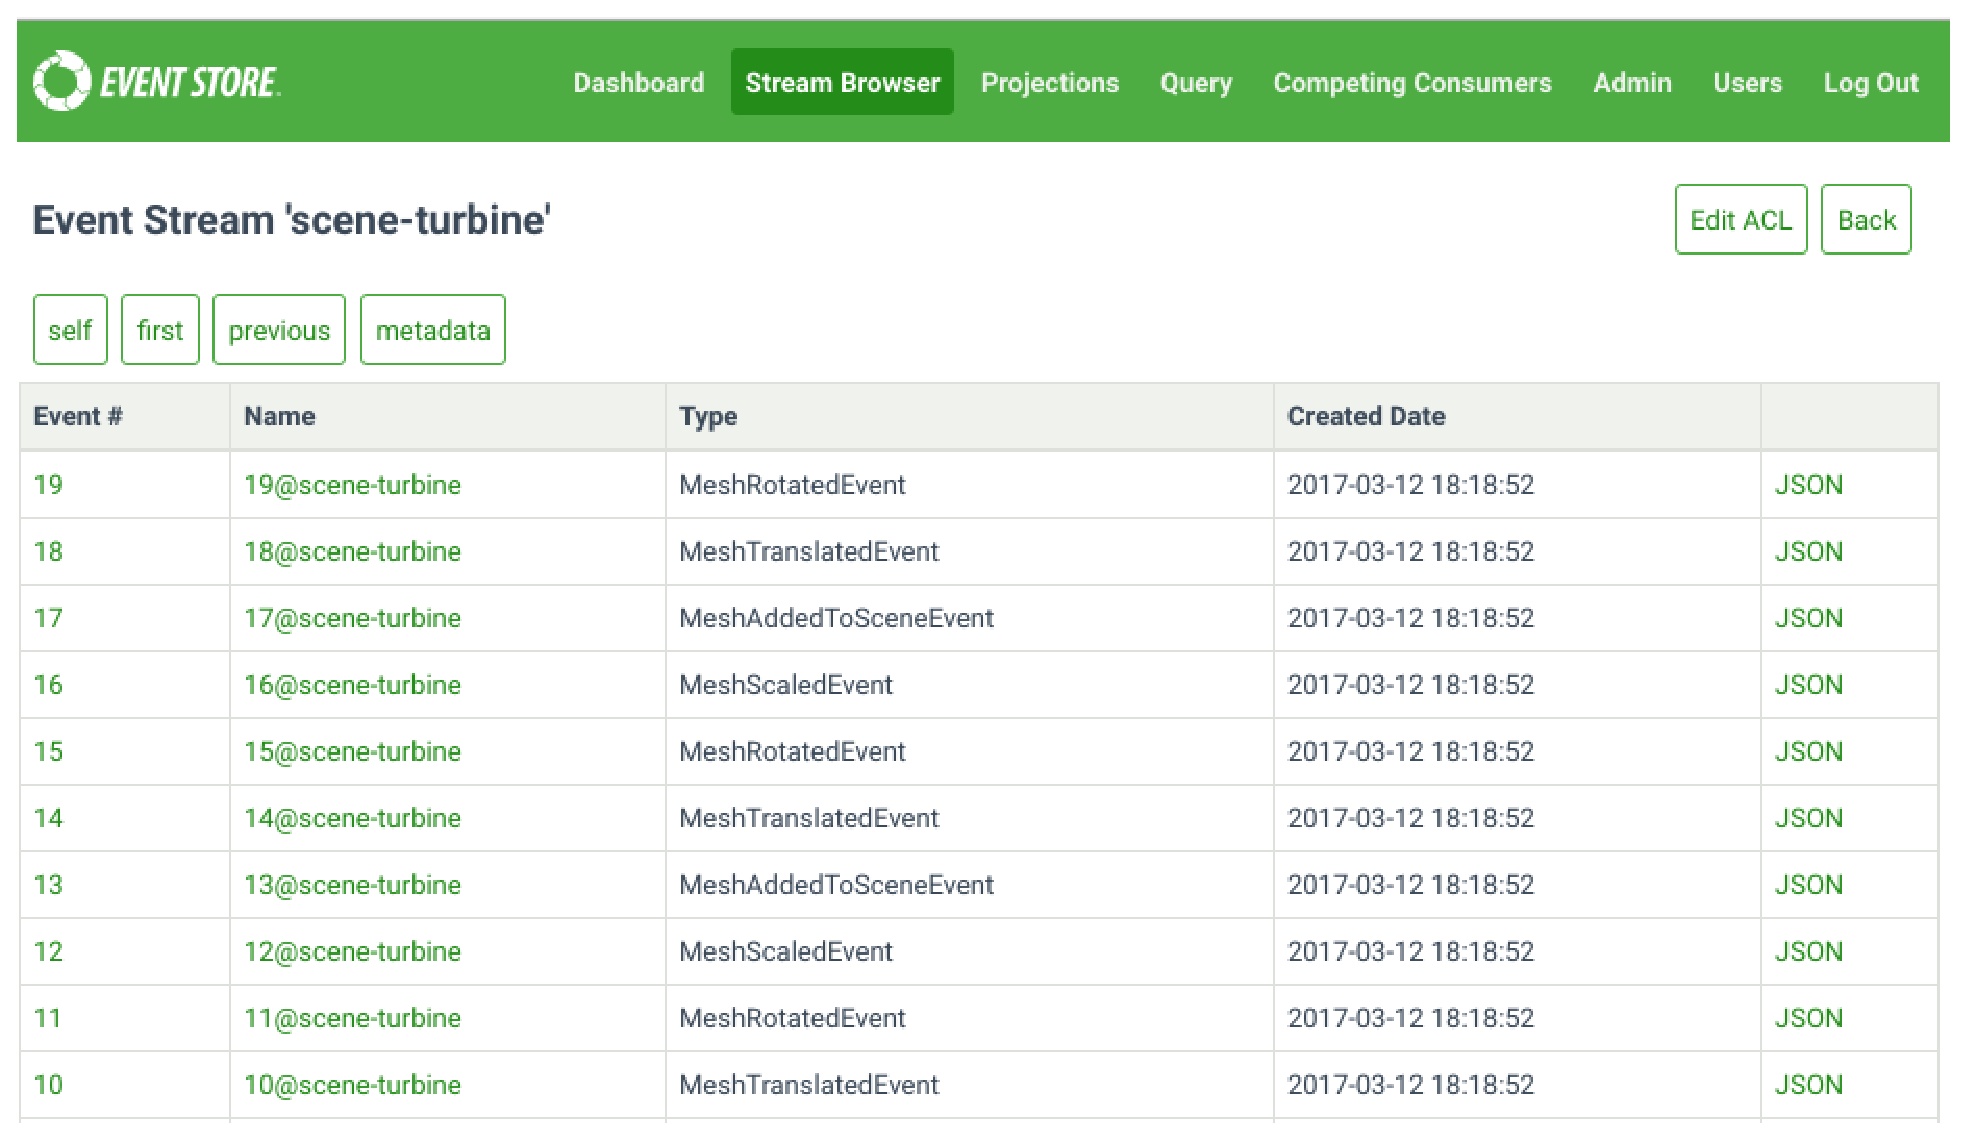
\includegraphics[width=\textwidth]{eps/eventstore.eps}
	\caption{Persistance long-terme (Event Store\textsuperscript{\textregistered}), 
		base de données/outil de monitoring}
	\label{fig:ui4}
\end{figure}


\paragraph{Analyse des interactions}
Les traces des utilisateurs récupérées au cours des expérimentations sont la base 
du travail d'analyse présenté ci-après. Ces traces, composées d'événements 
générés par les utilisateurs, permettent de savoir qui (Figure \ref{petita}) a fait quoi 
(Figure \ref{petitb}) lors des sessions collaboratives. Généralement, le \og qui\fg{} 
est assez facile à retrouver lors de la récupération des traces. Le \og quoi\fg{} 
en revanche nécessite que les notifications aient une signification précise et proche 
du métier. Grâce au travail de découpage et de dénomination des événements 
effectué en amont, le journal d'événements (\textit{log}) indique précisément tout 
ce qui s'est passé lors de la session du point de vue du métier. Cette 
fonctionnalité est intéressante dans le contexte de la traçabilité des données et 
lors d'audits sur l'assemblage. 

\begin{figure}[]
	\centering
	
	\subfloat[Par 
	utilisateur]{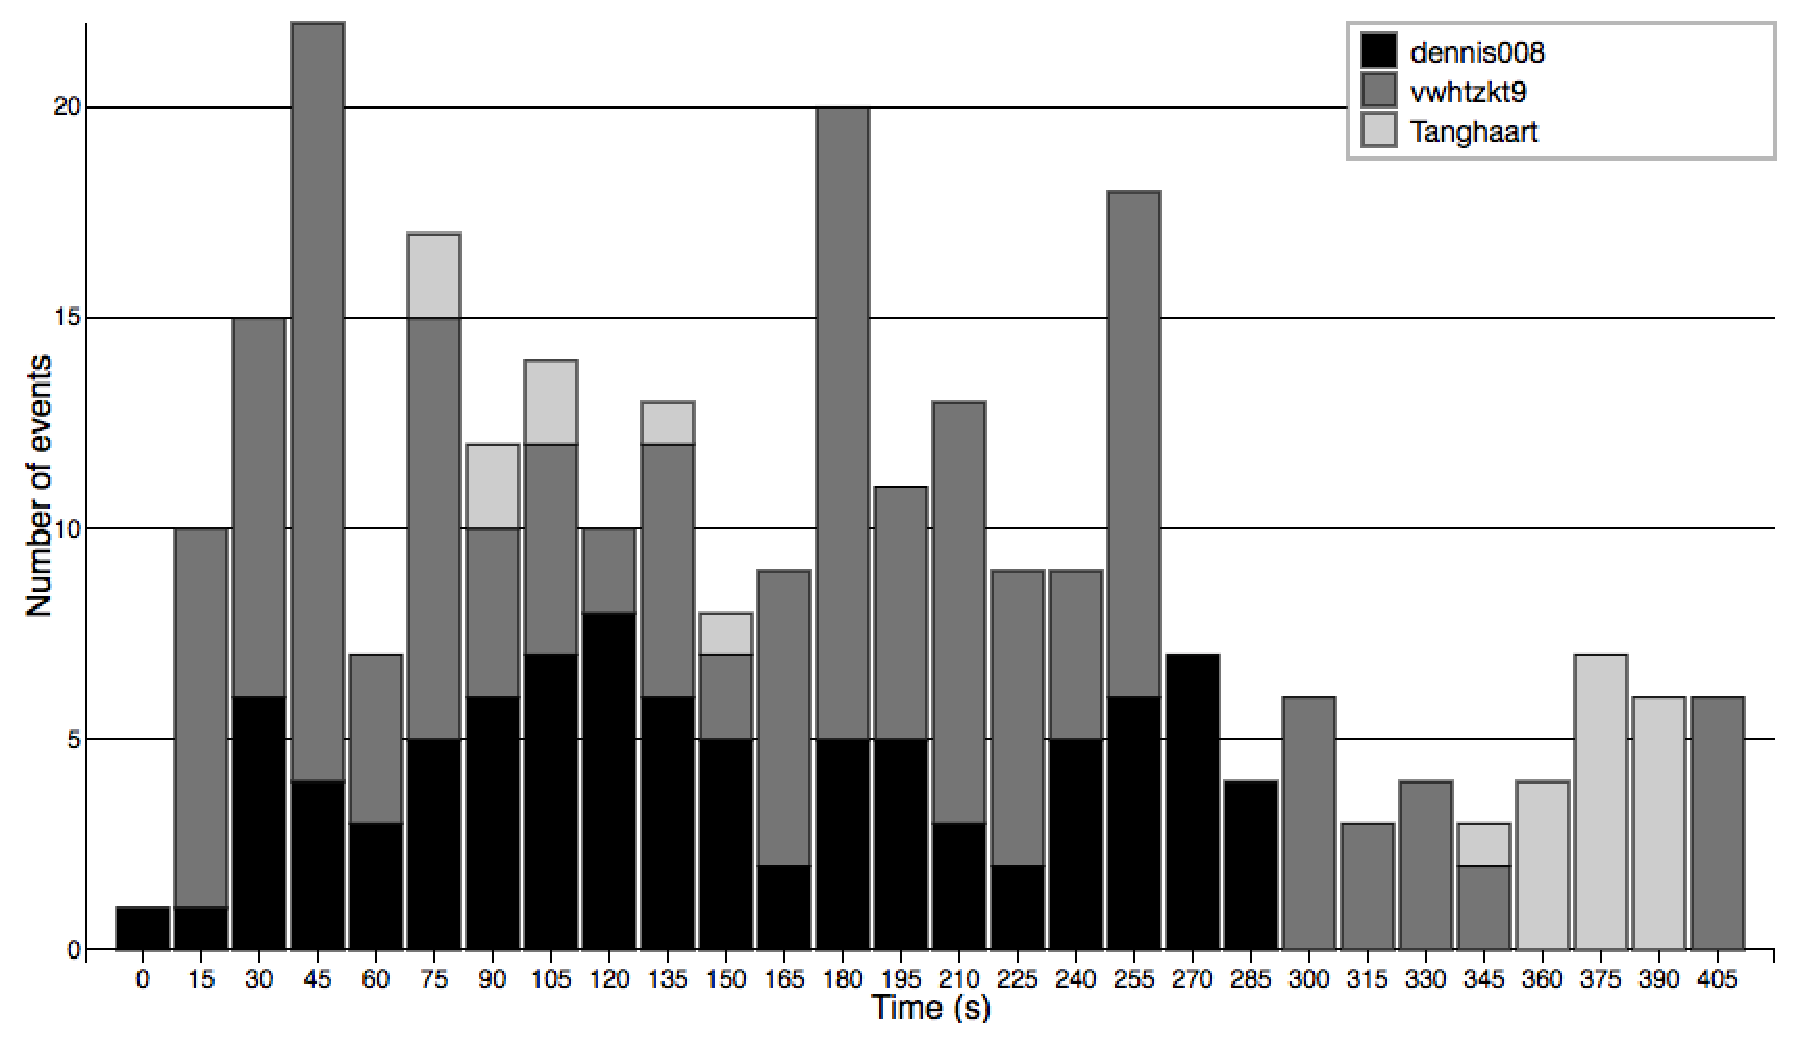
\includegraphics[width=\columnwidth]{eps/byuser.eps}\label{petita}}
	\\
	\subfloat[Par type 
	d'événement]{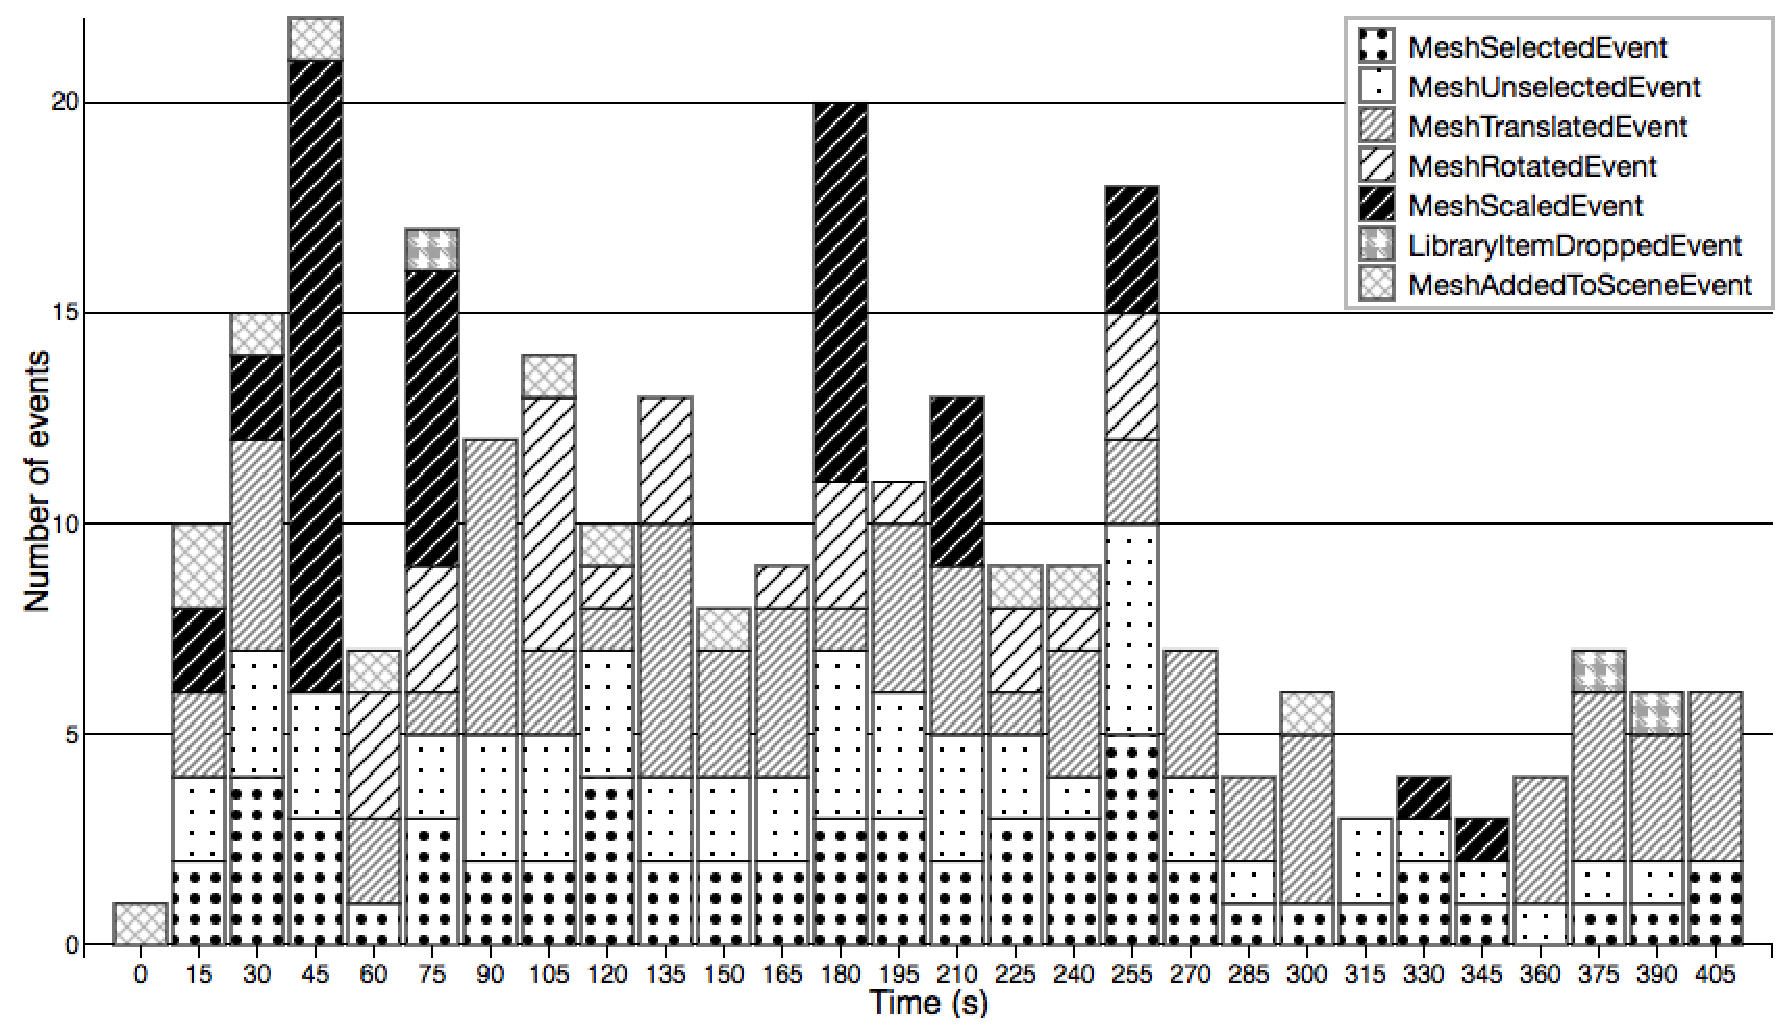
\includegraphics[width=\columnwidth]{eps/byevents.eps}\label{petitb}}
	\caption{Résumé d'une session collaborative au cours du temps}
	\label{fig:collabsession}
\end{figure}

La Figure \ref{fig:collabsession} montre deux angles d'enregistrement d'une session 
sur le modèle \textit{living room}. Au début de la session, beaucoup d'objets sont 
ajoutés (\textit{meshAddedToSceneEvent}). Seul un utilisateur a ajouté un objet 
en utilisant la fonctionnalité pour déposer un objet à un endroit spécifique de la 
scène (\textit{meshDropped}). Le nombre d'événements concernant la sélection et 
la désélection est à peu près similaire. La différence s'explique par 
le fait que l'événement de désélection n'est pas déclenché lorsque l'utilisateur 
change d'objet sélectionné. En effet, la désélection n'est pas effectuée 
explicitement par l'utilisateur. 
Dans les premiers moments, les participants ont fortement interagi 
(jusqu'à 20 événements en 15 secondes). Cela s'explique par le recours massif à 
l'ajout d'objets dans la scène pour composer le modèle et la mise à l'échelle de 
ceux-ci (causé par le positionnement arbitraire des objets de la bibliothèque). 
Ensuite, les trois utilisateurs interagissent ensemble durant quelques
minutes avant que l'un d'entre 
eux ne quitte et ne revienne quelques secondes plus tard (informations 
récupérées à partir du journal d'événements lié aux agrégats utilisateurs). Enfin, la diminution du nombre d'événements montre la fin de l'activité, les utilisateurs achevant 
la tâche et ajustant les derniers objets.

L'implication d'un utilisateur peut être perçue par le prisme de la fréquence de ses 
contributions et la variété de fonctionnalités utilisées, c.à.d. les différents 
types d'événements produits. L'analyse d'une session apporte plusieurs indicateurs 
tout au long de la session. Par exemple, l'absence d'un utilisateur pendant une 
longue période peut indiquer une déconnexion. Ou encore, l'utilisation trop 
fréquente d'un type d'événements (ou d'un motif d'événements répété) peut montrer 
une faiblesse de l'ergonomie de l'interface. Ce dernier aspect est illustré par un exemple dans la Figure \ref{petitb} à 45s, où un nombre élevé de 
MeshScaledEvent est détecté. \textit{A posteriori}, il est possible de constater  
que la fonctionnalité n'était pas suffisamment calibrée pour l'échelle du modèle et 
nécessitait plusieurs manipulations pour réaliser la bonne transformation.

	\begin{figure}[]
		\centering
		\includegraphics[width=1\columnwidth]{eps/questionnaire.eps} 
		\caption{Résultats des questionnaires collectés}
		\label{fig:questionnaire}
	\end{figure}


\paragraph{Questionnaires}
Après chaque expérimentation, le participant a rempli directement un questionnaire 
à propos de la phase \textit{Solo} et des phases \textit{Collaboration} qu'il a 
effectuées via le formulaire en ligne. Les résultats obtenus sont compilés dans la 
Figure \ref{fig:questionnaire} sous la forme de boîte à moustaches. Cette 
représentation est un moyen rapide de se figurer le profil essentiel des résultats 
des mesures quantitatives effectuées.

Globalement, les tâches ont été réalisées plus rapidement et plus efficacement 
de manière collaborative (\textit{Collaboration}) que seul (\textit{Solo}). La facilité 
d'utilisation et la simplicité de l'interface sont également soulignées positivement 
par plusieurs utilisateurs. 

Parmi les retours d'expérience négatifs, l'instabilité du réseau a parfois amené un 
peu de frustration chez certains participants. 
Cependant, les participants ont trouvé que la cohérence de l'environnement lors de 
la collaboration et la récupération des données était plus qu'acceptable. Cette 
remarque s'accompagne également du fait que la distribution des données s'est 
effectuée sans effets de bord, leur permettant de coopérer efficacement, avec peu 
de conflits détectés.

Durant l'une des expérimentations en phase \textit{Collaboration}, un 
participant a affiché à certains moments une latence de plus de 10s. ; mais 
le groupe nous a notifié que cela n'avait pas affecté la collaboration. Pour 
l'ensemble des expérimentations, quelques conflits ont été levés sur différentes 
opérations et à différents niveaux. 
Sur le réseau, la détection des conflits (mauvaise version, désynchronisation), la 
politique en place consiste à reconstruire l'état de l'application avant le conflit, i.e. 
jusqu'au dernier événement qui n'est pas en conflit, pour pouvoir resynchroniser 
les utilisateurs sur une base stable. Cette mécanique qui peut sembler 
envahissante n'a pas dérangé les utilisateurs lors de la modélisation.
Pour pallier l'absence de résolution automatique de conflit, les utilisateurs ont été 
mis a contribution dans les cas de désaccords (opérations opposées sur le même 
objet) : la résolution du conflit passe par un canal externe (chat) pour que les 
utilisateurs se mettent d'accord. Cette connaissance du métier n'est donc pas 
intégrée au système.


Dans toutes les expérimentations menées, le but a été atteint dans 
un même ordre de temps (10-12 minutes). La facilité d'utilisation du système est 
bien notée, mais il reste encore quelques aspects à améliorer notamment lors des 
désynchronisation, aucun affichage ne prévient l'utilisateur ou encore la 
sensibilisation à l'historique des objets manipulés. 
Pour modérer ces résultats, il est important de rappeler que les modèles utilisés 
ne sont pas très complexes et que tous les participants étaient débutants sur le 
système et parfois néophytes en modélisation 3D.
Le fait que l'application repose sur des technologies web a également joué en 
faveur de l'appropriation de l'application, car il a semblé assez naturel aux 
participants de se rendre à l'adresse internet donnée (sans rien installer) pour 
effectuer les tâches en manipulant un média (3D) inhabituel pour ce genre de 
plateformes. 
De plus, on peut également supposer que le prototype créé pour l'expérimentation 
correspond bien à l'objectif d'assemblage coopératif d'objets \gls{3D} puisque les 
tâches ont été réalisées rapidement. Sur une échelle de \og non-interactif \fg{} à 
\og temps réel\fg{} les participants ont qualifié l'application de \og quasi temps 
réel\fg{}. 

La satisfaction générale à propos de l'expérimentation et la satisfaction concernant 
la collaboration et l'expérience utilisateur peuvent être des indicateurs sur le fait 
que les participants ont apprécié positivement les épreuves proposées durant 
l'expérimentation. 
Quant à savoir si le nombre d'utilisateurs améliore à la fois l'efficacité et la rapidité 
du complètement de la tâche, les participants ont généralement été d'accord.

\subsection{Conclusion de l'expérimentation 2}

Les différentes phases de l'expérimentation amène le participant à prendre en 
main rapidement le prototype (Section \ref{sec:task-based-ui}). 
Le protocole, qui en proposant plusieurs épreuves sur différents modèles, offre un
large panel de situations liées aux cas d'études permettant d'évaluer les capacités 
de coordination et de coopération dans la réalisation des tâches.

L'expérimentation, construite sous l'angle de l'expérience utilisateur, propose ainsi 
d'évaluer l'utilisabilité de l'interface et les effets de l'architecture réseau choisi 
lors de l'implantation du modèle événementiel. 
Les utilisateurs ont globalement exprimé leur satisfaction concernant leur 
expérience générale : objectifs atteints, interface facile à prendre en main, 
collaboration facilitant la réalisation de la tâche. 
Concernant l'architecture réseau pour la collaboration, ils ont souligné la bonne 
récupération du système dans les cas de désynchronisation. Ces derniers 
n'apparaissent que lors d'une sélection multi-utilisateur du même agrégat et sont 
donc plutôt rares. De plus, les utilisateurs étant sensibilisés (par exemple : les 
boîtes englobantes de sélection en couleur) au fait qu'un autre utilisateur a déjà 
sélectionné l'objet, ils sont ainsi prévenus de l'occurrence potentielle de conflits. 







\section{Comparaison entre l'expérimentation 1 et l'expérimentation 2}

Les deux expérimentations présentées concernent le même cas d'étude mais 
reposent sur deux prototypes conçus sur la base de modèles utilisant des 
paradigmes différents. 

L'expérimentation 1 repose sur un modèle orienté états et présente principalement 
une preuve de concept et de faisabilité concernant l'architecture de communication 
hybride. Le passage à l'échelle est limité car le réseau est un maillage 
complet, ce qui sollicite beaucoup les pairs. Le serveur, lié à la base de données, 
reçoit également beaucoup de requêtes, tant en écriture qu'en lecture. Le 
mécanisme de verrouillage évite les conflits de sélection multi-utilisateurs, mais 
restreint l'accès aux objets de la scène aux collaborateurs. 


L'expérimentation 2 repose sur un modèle orienté événements et présente deux 
aspects des contributions développées dans cette thèse. Les événements 
produits permettent de décrire finement ce qui se passe durant la 
collaboration grâce à l'implantation des principes du \gls{DDD}. L'analyse est 
possible grâce aux outils dérivés du \gls{CQRS}. En cela, beaucoup d'aspects liés 
à l'observation de l'expérience utilisateur lors de la collaboration sont implicitement 
présents dans le prototype. La gestion des événements au sein du réseau est 
effectuée dans d'un journal d'événements 
partagé, dont la cohérence repose sur l'ordre causal des événements d'un 
agrégat.


Entre l'expérimentation 1 et l'expérimentation 2, le changement de paradigme a 
apporté aux différents utilisateurs de nouvelles fonctionnalités permettant d'améliorer leur 
expérience de collaboration, notamment du point de vue de la gestion des 
données métier. Par exemple, la validation systématique de leurs commandes à la 
base de chaque action dans l'expérimentation 2 évite de générer des événements 
problématiques. Cela est intensifié par l'utilisation de 
technologies comme JavaScript dans un navigateur web où il est très facile 
d'injecter du code permettant d'effectuer des actions sans passer par l'\gls{IU}. Notamment lorsque l'utilisateur passe par l'\gls{IU}, les erreurs de saisies sont plus
fréquentes. D'autre part, la gestion de la cohérence utilisée dans 
l'expérimentation 2 est beaucoup plus permissive que celle de l'expérimentation 1. 
Les utilisateurs ont de ce fait exprimé moins de frustration. Enfin, 
dans l'expérimentation 2, les participants ont produit de plus grosses quantités de 
données sans ressentir de frustration, de latence excessive ou de problème de 
gel de fenêtre.
L'expérimentation 2 ajoute des mécanismes de sensibilisation à la présence des 
autres utilisateurs par rapport à l'expérimentation 1 qui participe à l'évitement de conflit. L'observation des participants indique qu'ils ont moins tenté de travailler 
sur des objets déjà en cours d'utilisation lorsque les mécanismes sont activés, et ils ont donc généré moins de conflits. 
Pour compenser l'autorité d'un utilisateur sur un objet par le mécanisme de 
verrouillage dans l'expérimentation 1, les utilisateurs se sont appuyés 
sur le mécanisme de sélection fantôme, leur permettant d'être  maîtres des 
contrôles notamment lors d'une sélection multi-utilisateurs.

%\chapter{Conclusion}
%!TEX root = main.tex
\chapter{Conclusion}
\chaptertable

Cette thèse présente une architecture évènementielle pour les \gls{EVC} sur le 
web. Les contributions de cette thèse sont multiples. Il y a d'une part les 
contributions scientifiques qui porte sur l'\gls{EDA} pour la 
modélisation 3D collaborative et d'autre part, il y a la présentation d'une 
architecture de communication hybride permettant de synchroniser les 
\glspl{EVC3D} sur le web de différents client.

Chacune de ces contributions est accompagnée de son implantation. 

De plus, la réalisation de plusieurs prototypes fonctionnant sur différents 
paradigme pour les expérimentation ont permis de montrer les avantages et 
inconvénients de ceux-ci.

Enfin, les expérimentations principalement portées sur l'étude des utilisateurs 
permet de souligner plusieurs aspects du modèle. Le premier est de montrer que 
l'intégration du métier a permis l'observation minutieuse du travail réalisé au sein 
de l'environnement. 

\begin{appendix}
	\chapter{Ressources pour l'implantation et les expérimentations}
	\section{Description des événements par agrégat dans 3DEvent}
	\begin{landscape}
\begin{table}[]
	
	\centering
	\caption{3DEvent : résumé des événements par agrégats}
	\label{tab:events}
	\begin{tabular}{lll}
		\toprule
		\textbf{événement}& \textbf{Nommage} & \textbf{Description} \\ \midrule
		\textbf{Agrégat Scène}     &                      &             \\ \hline
		Scène créée &  sceneCreated                  & Une scène a été 
		créée            \\
		Scène supprimée &        sceneRemoved              &  Une scène a été 
		supprimée           \\
		Scène renommée &     sceneRenamed                 &     Une scène a été 
		renommée        \\
		\textbf{Agrégat Maillage}  &                      &             \\ \hline
		Maillage ajouté &     meshAdded                 
		&  \begin{tabular}[c]{@{}l@{}} Un maillage a été ajouté dans la Scène à 
		partir \\d'une géométrie de la 
		bibliothèque \end{tabular}  \\
		Maillage déposé &     meshDropped               
		&      \begin{tabular}[c]{@{}l@{}} Un maillage a été déposé dans 
		l'environnement 3D\\ de la Scène à 
		partir d'une géométrie de la bibliothèque \end{tabular} \\
		Maillage supprimé & meshRemoved       &           Un maillage a été 
		supprimé de la Scène   \\
		Maillage translaté &   meshTranslated  	 &    Un maillage a 
		subit une translation dans la Scène         \\
		Maillage pivoté &      meshRotated                &     Un maillage a 
		subit une rotation dans la Scène              \\
		Maillage mis à l'échelle &  meshScaled           &      Un maillage a 
		subit une homothétie dans la Scène         \\
		\textbf{Agrégat Géométrie} &                      &             \\ \hline
		Géométrie importé dans la bibliothèque &  geometryImported           &        
		\begin{tabular}[c]{@{}l@{}} Une géométrie est créée à partir d'un fichier 
		importé par\\ 
		un utilisateur et ajoutée à la bibliothèque de la 
		Scène \end{tabular}     \\
		\textbf{Agrégat Utilisateur}        &                      &            \\ \hline
		Utilisateur créé&   userCreated                   &        Un utilisateur a été créé 
		dans l'application    \\
		Scène rejointe par utilisateur&     userJoinedScene                 &      Un 
		utilisateur a rejoint une scène       \\
		Scène quittée par utilisateur&        userLeftScene              &    Un utilisateur 
		a quitté une scène         \\
		Nom modifié &         usernameChanged           &     Un utilisateur a modifié 
		son nom        \\
		Couleur modifiée &       colorChanged                  &      Un utilisateur a 
		modifié son code couleur       \\ \bottomrule
	\end{tabular}
\end{table}

\end{landscape}

\section{Messages réseaux pour la synchronisation des Event Stores}

\begin{table}[h]
	\centering
	\small
	\caption{Type de messages lors de la synchronisation}
	\label{table:messagetype}
	\begin{tabular}{ll}
		\toprule
		\textbf{Message}                & \textbf{Description} \\ \hline
		STREAM\_SYNC\_ASK      &  Demande de synchronisation d'un 
		\textit{stream}           \\
		CHUNK                  &     Réception d'une donnée \textit{chunk})        
		\\
		READY\_ASK             &      Prêt pour la démarrer la demande de 
		données de 
		sync.        \\
		READY                  &       Prêt pour démarrer la réception de 
		données de 
		sync.      \\
		ALL\_EVENTS\_SYNC\_ASK &     Demande de toutes les données 
		typées 
		événement           \\
		EVENTS\_SYNC           &        Réception de données (en cours de 
		synchronisation)       \\
		META\_DATA\_ASK        &     Demande de métadonnées       \\
		META\_DATA             &      Réception de métadonnées       \\
		SYNC                   &      Réception de données (en cours de 
		synchronisation)         \\
		EVENT                  &     Réception d'une donnée typée 
		événement        \\
		END\_SYNC              & Fin de la synchronisation \\ \bottomrule
	\end{tabular}
\end{table}
\todo{parler des tableaux}

\begin{table}[h]
	\centering
	\caption{Statut du n\oe ud}
	\label{table:nodestatus}
	\begin{tabular}{ll}
		\toprule
		\textbf{Message}             & \textbf{Description} \\ \midrule
		ERROR               &      En erreur (désynchronisation)       \\
		READY               &       Prêt à recevoir des messages      \\
		META\_DATA\_ASK     &      En demande de métadonnées       \\
		META\_DATA\_RECEIVE &      En réception de métadonnées       \\
		CLOSE               &     Déconnecté (connexion fermée)        \\
		RECEIVE\_SYNC       &      En réception de données à synchroniser    \\
		CONNECTED           &      Connecté (connexion ouverte)        \\
		INIT                &     Initialisation   \\
		OK                  &    Connecté et synchronisé      \\
		SEND\_SYNC          &    En demande de synchronisation         \\
		END\_SYNC           &      Synchronisation terminée      \\ \bottomrule
	\end{tabular}
\end{table}

\pagebreak
\section{Expérimentation 2 : User study questionnaire}
\label{app:quest}
Seven-points scale questions from 1 (don't agree) to 7 (agree):
\begin{itemize}
	\item Did you enjoy this?
	\item After trial, I was confident to do object manipulation in 3D virtual 
	environment?
	\item App learning: I am satisfied with the ease of use of the application
	\item App learning: It was easy to learn the tool
	\item Solo: I completed the task quickly
	\item Solo: I completed the task efficiently
	\item Collaboration: I contributed to complete the task quickly
	\item Collaboration: I contributed to complete the task efficiently
	\item In general, I am satisfied with the collaboration experience
	\item In general, The collaboration quality was pleasant in terms of LATENCY
	\item In general, The collaboration quality was pleasant in terms of 
	CONSISTENCY
	\item In general, The collaboration quality was pleasant in terms of RECOVERY
\end{itemize}
Other questions:
\begin{itemize}
	\item General efficiency is improved with the number of users?
	\item General speed is improved with the number of users?
	\item I would qualify this application: Non interactive/Interactive/Near 
	real-time/Real-time
	\item Negative/positive/comments feedbacks
\end{itemize}


\end{appendix}

\backmatter

\bibliographystyle{apalike-fr}
%	\bibliography{references}
\bibliography{mendeley}
\end{document}